% Options for packages loaded elsewhere
% Options for packages loaded elsewhere
\PassOptionsToPackage{unicode}{hyperref}
\PassOptionsToPackage{hyphens}{url}
\PassOptionsToPackage{dvipsnames,svgnames,x11names}{xcolor}
%
\documentclass[
]{article}
\usepackage{xcolor}
\usepackage{amsmath,amssymb}
\setcounter{secnumdepth}{3}
\usepackage{iftex}
\ifPDFTeX
  \usepackage[T1]{fontenc}
  \usepackage[utf8]{inputenc}
  \usepackage{textcomp} % provide euro and other symbols
\else % if luatex or xetex
  \usepackage{unicode-math} % this also loads fontspec
  \defaultfontfeatures{Scale=MatchLowercase}
  \defaultfontfeatures[\rmfamily]{Ligatures=TeX,Scale=1}
\fi
\usepackage{lmodern}
\ifPDFTeX\else
  % xetex/luatex font selection
\fi
% Use upquote if available, for straight quotes in verbatim environments
\IfFileExists{upquote.sty}{\usepackage{upquote}}{}
\IfFileExists{microtype.sty}{% use microtype if available
  \usepackage[]{microtype}
  \UseMicrotypeSet[protrusion]{basicmath} % disable protrusion for tt fonts
}{}
\makeatletter
\@ifundefined{KOMAClassName}{% if non-KOMA class
  \IfFileExists{parskip.sty}{%
    \usepackage{parskip}
  }{% else
    \setlength{\parindent}{0pt}
    \setlength{\parskip}{6pt plus 2pt minus 1pt}}
}{% if KOMA class
  \KOMAoptions{parskip=half}}
\makeatother
% Make \paragraph and \subparagraph free-standing
\makeatletter
\ifx\paragraph\undefined\else
  \let\oldparagraph\paragraph
  \renewcommand{\paragraph}{
    \@ifstar
      \xxxParagraphStar
      \xxxParagraphNoStar
  }
  \newcommand{\xxxParagraphStar}[1]{\oldparagraph*{#1}\mbox{}}
  \newcommand{\xxxParagraphNoStar}[1]{\oldparagraph{#1}\mbox{}}
\fi
\ifx\subparagraph\undefined\else
  \let\oldsubparagraph\subparagraph
  \renewcommand{\subparagraph}{
    \@ifstar
      \xxxSubParagraphStar
      \xxxSubParagraphNoStar
  }
  \newcommand{\xxxSubParagraphStar}[1]{\oldsubparagraph*{#1}\mbox{}}
  \newcommand{\xxxSubParagraphNoStar}[1]{\oldsubparagraph{#1}\mbox{}}
\fi
\makeatother
\usepackage{listings}
\newcommand{\passthrough}[1]{#1}
\lstset{defaultdialect=[5.3]Lua}
\lstset{defaultdialect=[x86masm]Assembler}


\usepackage{longtable,booktabs,array}
\newcounter{none} % for unnumbered tables
\usepackage{calc} % for calculating minipage widths
% Correct order of tables after \paragraph or \subparagraph
\usepackage{etoolbox}
\makeatletter
\patchcmd\longtable{\par}{\if@noskipsec\mbox{}\fi\par}{}{}
\makeatother
% Allow footnotes in longtable head/foot
\IfFileExists{footnotehyper.sty}{\usepackage{footnotehyper}}{\usepackage{footnote}}
\makesavenoteenv{longtable}
\usepackage{graphicx}
\makeatletter
\newsavebox\pandoc@box
\newcommand*\pandocbounded[1]{% scales image to fit in text height/width
  \sbox\pandoc@box{#1}%
  \Gscale@div\@tempa{\textheight}{\dimexpr\ht\pandoc@box+\dp\pandoc@box\relax}%
  \Gscale@div\@tempb{\linewidth}{\wd\pandoc@box}%
  \ifdim\@tempb\p@<\@tempa\p@\let\@tempa\@tempb\fi% select the smaller of both
  \ifdim\@tempa\p@<\p@\scalebox{\@tempa}{\usebox\pandoc@box}%
  \else\usebox{\pandoc@box}%
  \fi%
}
% Set default figure placement to htbp
\def\fps@figure{htbp}
\makeatother





\setlength{\emergencystretch}{3em} % prevent overfull lines

\providecommand{\tightlist}{%
  \setlength{\itemsep}{0pt}\setlength{\parskip}{0pt}}



 
\usepackage[]{natbib}
\bibliographystyle{styles/icml2026}


% 中文支持（需 xelatex 编译）
\usepackage{ctex}
\usepackage{microtype}
\usepackage{graphicx}
\usepackage{subcaption}
\usepackage{booktabs}
\usepackage{hyperref}
\newcommand{\theHalgorithm}{\arabic{algorithm}}
\usepackage[preprint]{styles/icml2026}
\PassOptionsToPackage{hyphens}{url}
\usepackage{url}
\usepackage{amsfonts}
\usepackage{amsmath}
\usepackage{amsthm}
\usepackage{nicefrac}
\usepackage{xcolor}
\usepackage{listings}
\usepackage{algorithm}
\usepackage{algorithmic}
\usepackage{enumitem}
\usepackage{multirow}
\usepackage{stfloats}
\usepackage{placeins}
\usepackage{tikz}
\usetikzlibrary{shapes,arrows,positioning,fit,backgrounds}
\usepackage{helvet}
\usepackage{tcolorbox}
\usepackage{pifont}
\newcommand{\cmark}{\textcolor{green!60!black}{\ding{51}}}
\newcommand{\xmark}{\textcolor{red!70!black}{\ding{55}}}
\definecolor{abstractbg}{HTML}{EEF3F9}
\newtcolorbox{headerpanel}{%
  colback=abstractbg,
  colframe=abstractbg,
  arc=8pt,
  boxrule=0pt,
  left=18pt, right=18pt, top=16pt, bottom=14pt,
  width=\textwidth,
  enlarge left by=0pt,
  enlarge right by=0pt,
}
\theoremstyle{definition}
\newtheorem{definition}{定义}[section]
\newcommand{\ara}{\textsc{Ara}}
\newcommand{\todo}[1]{\textcolor{red}{\textbf{[TODO: #1]}}}
\newcommand{\layer}[1]{\texttt{/#1}}
\newcommand{\cmd}[1]{\texttt{ara~#1}}
\newcommand{\storytax}{\emph{Storytelling Tax}}
\newcommand{\engtax}{\emph{Engineering Tax}}
\lstset{
  basicstyle=\ttfamily\scriptsize,
  breaklines=true,
  frame=single,
  framesep=3pt,
  columns=fullflexible,
  backgroundcolor=\color{gray!5},
  keywordstyle=\color{blue!70!black},
  commentstyle=\color{green!50!black},
  stringstyle=\color{red!60!black},
}
\icmltitlerunning{The Last Human-Written Paper: Agent-Native Research Artifacts}
\makeatletter
\@ifpackageloaded{caption}{}{\usepackage{caption}}
\AtBeginDocument{%
\ifdefined\contentsname
  \renewcommand*\contentsname{Table of contents}
\else
  \newcommand\contentsname{Table of contents}
\fi
\ifdefined\listfigurename
  \renewcommand*\listfigurename{List of Figures}
\else
  \newcommand\listfigurename{List of Figures}
\fi
\ifdefined\listtablename
  \renewcommand*\listtablename{List of Tables}
\else
  \newcommand\listtablename{List of Tables}
\fi
\ifdefined\figurename
  \renewcommand*\figurename{Figure}
\else
  \newcommand\figurename{Figure}
\fi
\ifdefined\tablename
  \renewcommand*\tablename{Table}
\else
  \newcommand\tablename{Table}
\fi
}
\@ifpackageloaded{float}{}{\usepackage{float}}
\floatstyle{ruled}
\@ifundefined{c@chapter}{\newfloat{codelisting}{h}{lop}}{\newfloat{codelisting}{h}{lop}[chapter]}
\floatname{codelisting}{Listing}
\newcommand*\listoflistings{\listof{codelisting}{List of Listings}}
\makeatother
\makeatletter
\makeatother
\makeatletter
\@ifpackageloaded{caption}{}{\usepackage{caption}}
\@ifpackageloaded{subcaption}{}{\usepackage{subcaption}}
\makeatother
\usepackage{bookmark}
\IfFileExists{xurl.sty}{\usepackage{xurl}}{} % add URL line breaks if available
\urlstyle{same}
% fallback for those not using the hyperref driver hyperxmp:
\makeatletter
\@ifundefined{xmpquote}{\newcommand{\xmpquote}[1]{#1}}{}
\makeatother
\hypersetup{
  colorlinks=true,
  linkcolor={blue},
  filecolor={Maroon},
  citecolor={Blue},
  urlcolor={Blue},
  pdfcreator={LaTeX via pandoc}}


\author{}
\date{}
\begin{document}


\twocolumn[
  \thispagestyle{plain}
  \begin{headerpanel}
    \raggedright
    % 标题
    {\sffamily\bfseries\fontsize{19}{23}\selectfont
      最后一篇人类撰写的论文：\\
      智能体原生研究构件\par
    }
    \vskip 12pt
    % 作者列表
    {\sffamily\bfseries\normalsize
      Jiachen Liu\textsuperscript{1,\,*},\ %
      Jiaxin Pei\textsuperscript{2},\ %
      Jintao Huang\textsuperscript{3},\ %
      Chenglei Si\textsuperscript{2},\ %
      Ao Qu\textsuperscript{4},\ %
      Xiangru Tang\textsuperscript{5},\ %
      Runyu Lu\textsuperscript{1},\ %
      Lichang Chen\textsuperscript{6},\ %
      Xiaoyan Bai\textsuperscript{7},\ %
      Haizhong Zheng\textsuperscript{8},\ %
      Carl Chen\textsuperscript{9},\ %
      Zhiyang Chen\textsuperscript{10},\ %
      Haojie Ye\textsuperscript{11},\ %
      Yujuan Fu\textsuperscript{12},\ %
      Zexue He\textsuperscript{2},\ %
      Zijian Jin\textsuperscript{13},\ %
      Zhenyu Zhang\textsuperscript{2},\ %
      Shangquan Sun\textsuperscript{14},\ %
      Maestro Harmon\textsuperscript{15},\ %
      Dianzhuo Wang\textsuperscript{16},\ %
      Qian-ze Zhu\textsuperscript{16},\ %
      Jianqiao Zeng,\ %
      Jiachen Sun\textsuperscript{17},\ %
      Mingyuan Wu\textsuperscript{18},\ %
      Baoyu Zhou\textsuperscript{19},\ %
      Chenyu You\textsuperscript{20},\ %
      Shijian Lu\textsuperscript{14},\ %
      Yiming Qiu\textsuperscript{21},\ %
      Fan Lai\textsuperscript{18},\ %
      Yuan Yuan\textsuperscript{22},\ %
      Yao Li\textsuperscript{23},\ %
      Junyuan Hong\textsuperscript{24},\ %
      Ruihao Zhu\textsuperscript{25},\ %
      Beidi Chen\textsuperscript{8},\ %
      Alex Pentland\textsuperscript{2},\ %
      Ang Chen\textsuperscript{1},\ %
      Mosharaf Chowdhury\textsuperscript{1},\ %
      Zechen Zhang\textsuperscript{16,\,15}\par
    }
    \vskip 6pt
    % 单位
    {\small
      \textsuperscript{1}University of Michigan,\ %
      \textsuperscript{2}Stanford University,\ %
      \textsuperscript{3}Ohio State University,\ %
      \textsuperscript{4}MIT,\ %
      \textsuperscript{5}Yale University,\ %
      \textsuperscript{6}Meta Superintelligence Labs,\ %
      \textsuperscript{7}University of Chicago,\ %
      \textsuperscript{8}Carnegie Mellon University,\ %
      \textsuperscript{9}University of Washington,\ %
      \textsuperscript{10}University of Toronto,\ %
      \textsuperscript{11}NVIDIA,\ %
      \textsuperscript{12}Meta,\ %
      \textsuperscript{13}New York University,\ %
      \textsuperscript{14}Nanyang Technological University,\ %
      \textsuperscript{15}Orchestra Research,\ %
      \textsuperscript{16}Harvard University,\ %
      \textsuperscript{17}LinkedIn,\ %
      \textsuperscript{18}UIUC,\ %
      \textsuperscript{19}Arizona State University,\ %
      \textsuperscript{20}Stony Brook University,\ %
      \textsuperscript{21}University of Hong Kong,\ %
      \textsuperscript{22}Boston College,\ %
      \textsuperscript{23}Portland State University,\ %
      \textsuperscript{24}National University of Singapore,\ %
      \textsuperscript{25}Cornell University\par
    }
    \vskip 14pt
    % 摘要正文（已内联）
    科学出版将分支式、迭代式的研究过程压缩为线性叙事，抛弃了探索过程中发现的大部分内容。这种编纂方式带来了两种结构性成本：一是\textbf{叙事税}，即失败的实验、被拒绝的假设以及分支探索过程被抛弃以适应线性叙事；二是\textbf{工程税}，即满足审稿人需求的叙述与满足智能体需求的规范之间的鸿沟导致关键的实现细节未被书写。这些成本对人类读者而言尚可容忍，但当AI智能体需要对已发表的工作进行理解、复现和扩展时，它们便成为关键障碍。我们提出\textbf{智能体原生研究构件（\ara{}）}，这是一种以可被智能体执行的研究包替代叙事性论文的协议，其结构围绕四个层展开：科学逻辑、具备完整规范的可执行代码、保留被编纂过程抛弃之失败的探索图谱，以及将每个论断锚定于原始输出的证据。三个机制支撑整个生态系统：\textbf{实时研究管理器}，在日常开发过程中捕获决策与死胡同；\textbf{\ara{} 编译器}，将既有PDF和代码仓库转换为 \ara{}；以及\textbf{\ara{} 原生审阅系统}，自动执行客观性检查（类似文本的语法检查器），从而使人类审稿人能够专注于重要性、新颖性和品味。在 PaperBench 和 RE-Bench 上，\ara{} 将问答准确率从 72.4\% 提升至 93.7\%，将复现成功率从 57.4\% 提升至 64.4\%。在 RE-Bench 的五项开放式扩展任务中，\ara{} 中保留的失败轨迹加速了研究进展，但也可能根据智能体自身的能力，限制有能力的智能体跳出先前运行的框架。
    \vskip 14pt
    % 通讯作者 / 代码页脚
    \noindent
    \parbox{0.70\linewidth}{%
      \noindent\textbf{通讯作者：}\ Jiachen Liu (\href{mailto:amberljc@umich.edu}{amberljc@umich.edu})\par
      \vskip 2pt
      \noindent\textbf{代码：}\ \href{https://github.com/AmberLJC/Agent-Native-Research-Artifact}{github.com/AmberLJC/Agent-Native-Research-Artifact}%
    }\hfill
    $\vcenter{\hbox{\sffamily\bfseries\small ARA Commons}}\,\vcenter{\hbox{
\includegraphics[height=30pt]{figures/brace-a_mark.png}}}$
  \end{headerpanel}
]

\ifdefined\hypersetup
  \hypersetup{pdftitle={The Last Human-Written Paper: Agent-Native Research Artifacts}}
\fi

\makeatletter
\global\icml@noticeprintedtrue
\makeatother

\section{引言}\label{sec-intro}

研究产生的是一个丰富、分支的知识对象：历经数月的假设检验与推翻，通过反复试错发现的实现技巧，在多个设计方案之间反复权衡，以及解释为何最终选择该方法的完整探索轨迹。
出版将这一对象编译为线性叙事
\citep{medawar1963fraud, canini2026stopwriting}，丢弃了失败的实验、隐性的工程知识以及分支探索过程，以迎合人类可读叙事的惯例
\citep{rosenthal1979filedrawer, franco2014publication}。
当论文的每一位消费者都是人类时，这种编译代价------源于文档化惯例而非特定文件格式的产物------尚可接受。
但当 AI
智能体需要例行阅读论文以理解领域、复现实验以验证发现、并将已发表方法扩展至新场景时
\citep{lu2024aiscientist, liu2026ainative}，这种代价便不可接受：每一项任务恰恰需要被编译所丢弃的知识（图
Figure~\ref{fig-overview}）。
更具体而言，这一编译过程带来了两类结构性代价。

\begin{figure}[!t]

\centering{

\pandocbounded{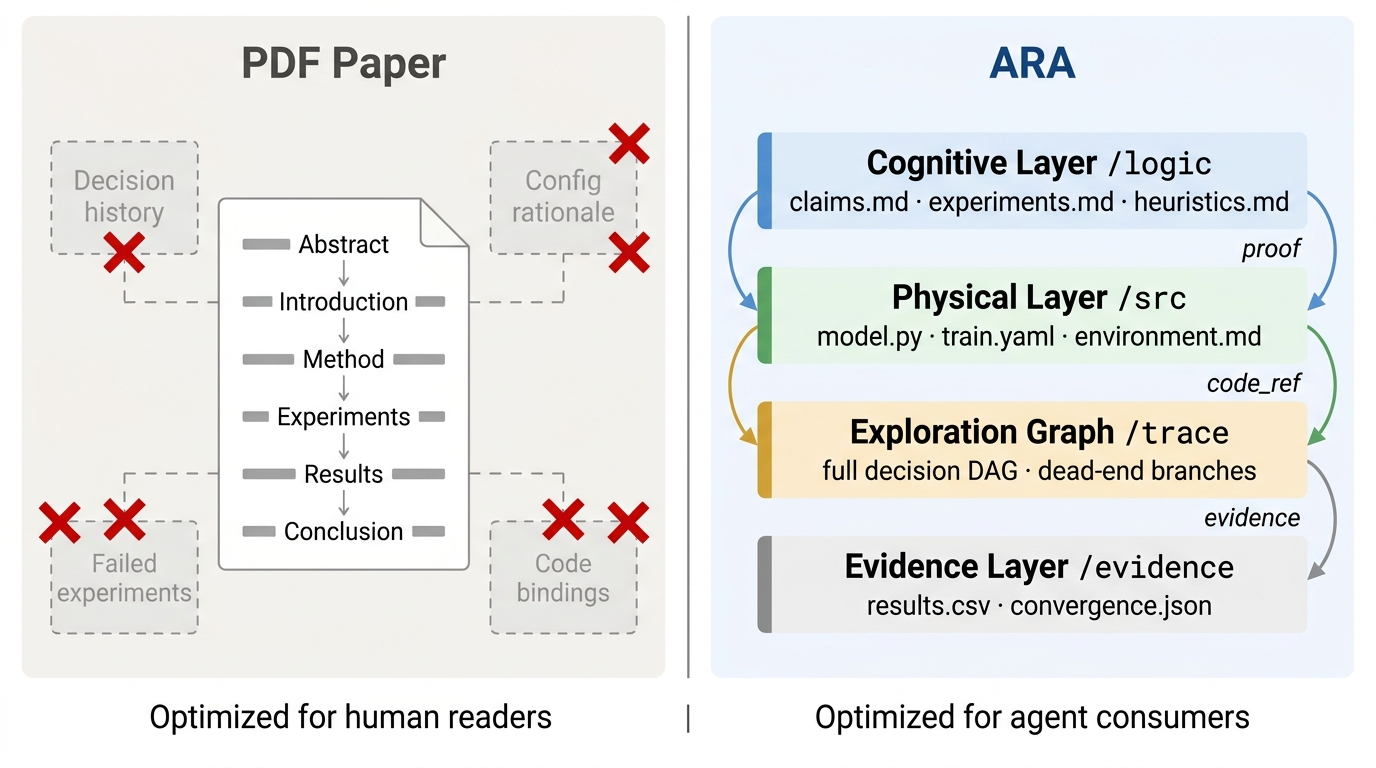
\includegraphics[keepaspectratio]{figures/fig_legacy_vs_ara_v6.png}}

}

\caption{\label{fig-overview}出版将丰富的研究对象编译为有损的叙事（左）；Ara
则将原始对象保存为高保真、智能体可执行的知识包（右）。}

\end{figure}%

其一是\textbf{叙事税}：将研究过程编译为叙事时，对研究过程知识造成的系统性抹除（图
Figure~\ref{fig-storytelling-tax}）。
研究并非线性推进------它在收敛到可发表结果之前，不断分支、回溯，并积累来之不易的失败知识
\citep{kuhn1962structure, medawar1963fraud}。
叙事编译将这一过程压扁为一条经过打磨的线性故事，丢弃了每一个失败的实验、被推翻的假设和被放弃的方向。
这种对成功的强调使失败无人记录；尽管现代平台能归档最终制品，但分支式的研究过程仍未被记录，导致不同研究团队独立重复发现同样的死胡同
\citep{rosenthal1979filedrawer, franco2014publication}。 我们基于 METR
的 eval-analysis-public 数据集 \citep{wijk2025rebench}
进行的分析------涵盖 21 个前沿模型在 RE-Bench 上的 24,008
次智能体运行------量化了这一代价（附录 \ref{sec-app-exploration-tax}
中给出了逐任务分解）：失败运行占总美元成本的 \textbf{90.2\%}（占总 token
量的 59.2\%），失败与成功运行的中位 token 比高达
\textbf{113\(\times\)}，无法获取先前失败记录的智能体必须独立重新发现每一个死胡同。
同样被丢弃的还有人类\emph{判断}在整个轨迹中的记录：每一次拒绝、修改和认可，都是关于何谓好的研究的偏好信号------一旦智能体承担了繁重的执行工作，这种信号便成为稀缺资源。叙事编译丢弃了这些信号；而保留的轨迹则将其呈现为结构化的监督信号，可跨项目累积复用。

其二是\textbf{工程税}：\emph{足以满足评审者}的文档与\emph{足以满足智能体}的文档之间的鸿沟（图
Figure~\ref{fig-info-gap}）。
论文以说服人类评审者所需的细节层级来传达其贡献；代码仓库提供了实现，但未提供执行所需的操作规范。
两者之间是隐性知识
\citep{polanyi1966tacit}------算法技巧、实现决策和配置选择------这些知识不存在于任何书面文档中，仅能通过直接与实验室接触或费力的逆向工程来传递。
我们通过将 PaperBench 中覆盖 23 篇 ICML 2024 论文的 8,921
条专家标注复现需求 \citep{starace2025paperbench} 与其源 PDF
逐条对照分类来量化这一鸿沟（附录 \ref{sec-app-gap-types}
中给出了逐类别分解和鸿沟类型分类法）：尽管已有广泛的制品共享，但仅有
\textbf{45.4\%} 的需求被完整规定。 代码开发是最欠规定的类别（充分率为
37.3\%），而仅缺失超参数一项就占所有鸿沟的 26.2\%（完整分解见附录
\ref{sec-app-gap-types}）：这揭示了论文写作精度（足以产生信念）与智能体操作精度（足以产生正确执行）之间的根本性错配
\citep{stodden2016enhancing, baker2016reproducibility}。

两类税负贯穿整个研究史一直存在，因为人类读者始终是那个带宽受限的层，负责处理庞大、非线性的研究轨迹。
如今，强大的 AI
智能体提供了一种更高效的、贴近人类的代理，能够以机器带宽代表读者处理研究轨迹，而三种趋势预示了这样的制品应当具备何种形态。
\textbf{第一}，AI
智能体已成为不可或缺的研究伙伴，与人类共同编写代码、运行实验、迭代假设
\citep{lu2024aiscientist}，LLM 的采用与各科学领域论文产出增长
23.7\%--89.3\% 相关
\citep{kusumegi2025scientific}；完整的研究轨迹（每一次失败、每一个实现技巧、每一项配置选择、每一次设计转向）如今被捕获为研究者与智能体会话中的机器可读文本，但尚无协议将其作为一等输出来保存。
\textbf{第二}，人类与 AI 智能体的信息需求存在分歧：人类略读摘要和图表
\citep{renear2009strategic}，而智能体受益于详尽信息，因为这些信息严格改善复现、验证和扩展，因此单个人类叙事优化的制品已无法同时服务二者。
\textbf{第三}，研究正扩展为大规模并行事业，智能体以机器速度分叉、扩展和合并彼此的工作，瓶颈从个体生产力转向制品的\emph{可操作性}：为顺序人类阅读而编译的叙事型
PDF，无法被分叉、差异比较或合并，但结构化的、无损的制品可以，从而使研究能够如软件般复合增长。

\begin{figure}[!t]

\centering{

\pandocbounded{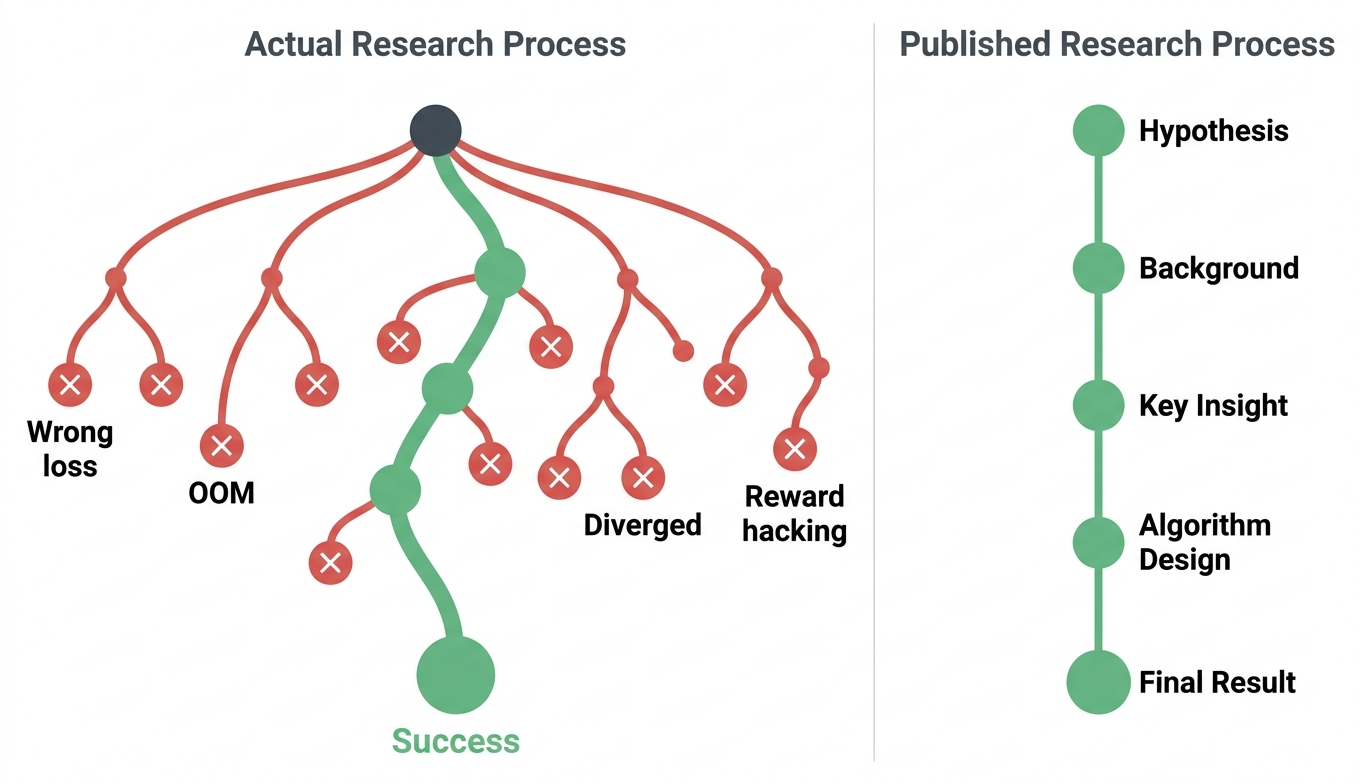
\includegraphics[keepaspectratio]{figures/fig_exploration_tax.png}}

}

\caption{\label{fig-storytelling-tax}叙事税：研究以包含死胡同的分支树形式推进（左），但出版将其编译为线性叙事（右），丢弃了所有失败知识。}

\end{figure}%

现有工作只解决了该问题的部分侧面。 FAIR 原则 \citep{wilkinson2016fair}
要求数据可发现、可访问，但对研究\emph{论证}的结构未作规定。 RO-Crate
\citep{soilandreyes2022rocrate} 将研究制品打包为档案束，而非可执行对象。
Nanopublications \citep{groth2010nanopub}
将原子性论断形式化，但缺少复现所需的执行层。 新兴的
\passthrough{\lstinline!AGENTS.md!} 标准 \citep{openai2025agentsmd}
为代码仓库提供了面向智能体的文档，但并未涉及研究本身的认知结构。
上述工作均未将科学逻辑、可执行代码和探索历史联合结构化为单一可操作对象（\ref{sec-related}）。

我们提出\textbf{智能体原生研究构件（\textsc{Ara}）}，一种将主要研究对象从叙事文档重塑为智能体可执行知识包的协议，论文则作为底层制品的编译视图（图
Figure~\ref{fig-overview}）。 \textsc{Ara}
将研究组织为四个相互耦合的层次：\emph{结构化科学逻辑}，将论文的概念抽象提炼为可查询的论断及其依赖图谱；\emph{可执行代码}，附带完整的操作规范；\emph{探索图谱}，保留叙事编译所丢弃的分支研究过程------失败的实验、被推翻的假设和设计转向；以及\emph{有据的证据}，将每一条论断与其原始实证输出相绑定。
在 \textsc{Ara}
制品上操作的智能体无需解析散文、逆向工程代码仓库和重新发现死胡同，即可直接查询结构化论断、执行声明式规范、并基于完整决策历史进行后续构建------这是一种设计目标不是被\emph{阅读}、而是被\emph{操作}的研究对象。

为构建围绕 \textsc{Ara} 的生态系统，我们开发了三种支撑机制。
\textbf{实时研究管理器}（\ref{sec-live-pm}）将研究决策和死胡同作为日常开发的自然副产品加以捕获，在不增加额外文档负担的前提下产出符合规范的制品。
\textbf{\textsc{Ara} 编译器}（Section~\ref{sec-ingestor}）将遗留
PDF、代码仓库和补充材料翻译为 \textsc{Ara}
格式，提供与现有出版生态的向后兼容。 \textbf{\textsc{Ara}
原生评审系统}（\ref{sec-review-system}）自动化结构验证和预算感知的复现（类似于散文的语法检查器），将专家注意力从机械核对重定向至判断------显著性、新颖性和品味
\citep{aczel2021billiondollar}。

\begin{figure}[!t]

\centering{

\pandocbounded{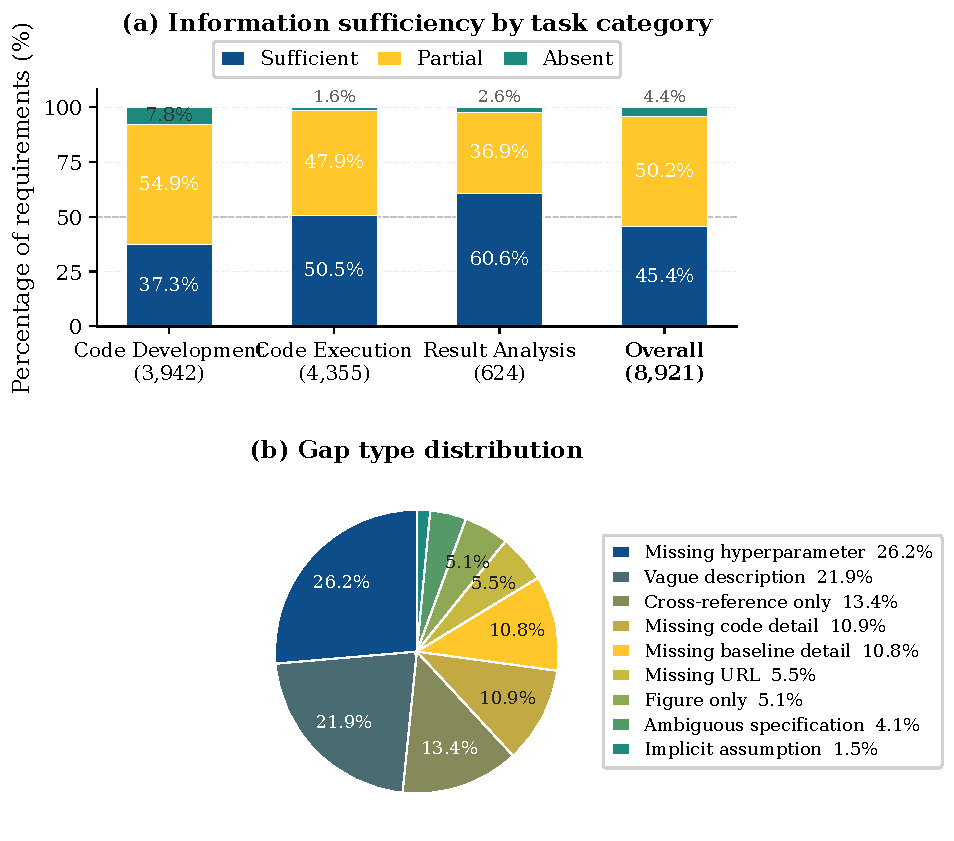
\includegraphics[keepaspectratio]{figures/fig_info_gap.pdf}}

}

\caption{\label{fig-info-gap}基于 8,921 条 PaperBench
需求的复现信息鸿沟。\textbf{(a)} PDF
系统性地欠规定代码开发任务。\textbf{(b)} 三种最大的鸿沟类型恰为 Ara
结构化层次所针对的类别。}

\end{figure}%

\paragraph{贡献。}\label{ux8d21ux732e}

\begin{itemize}
\tightlist
\item
  我们识别了将研究编译为叙事的两类结构性代价------\textbf{叙事税}和\textbf{工程税}------并引入\textbf{智能体原生研究构件（\textsc{Ara}）}：一种将主要研究对象从叙事文档重塑为智能体可执行知识包，并组织为四个相互耦合层次的协议（Section~\ref{sec-protocol}）。
\item
  我们开发了三种支撑机制：\textbf{实时研究管理器}（\ref{sec-live-pm}），在日常开发中捕获研究决策；\textbf{\textsc{Ara}
  编译器}（Section~\ref{sec-ingestor}），将遗留 PDF 和代码仓库翻译为
  \textsc{Ara} 格式；以及 \textbf{\textsc{Ara}
  原生评审系统}（\ref{sec-review-system}），自动执行客观验证（类似于散文的语法检查器），使人类评审者得以聚焦于判断。
\item
  我们在三个研究效用层次上评估
  \textsc{Ara}（\ref{sec-eval}）：\emph{理解}（智能体从制品中可提取到什么）、\emph{复现}（智能体能否重新执行论文的实验）、以及\emph{扩展}（智能体能否在已有结果基础上进一步构建并发现真正新的发现------研究的根本目标）。在所有三个层次上，基于
  \textsc{Ara} 操作的智能体始终优于阅读论文 PDF
  及其关联代码仓库的智能体。
\end{itemize}

\section{\texorpdfstring{\textsc{Ara} 协议}{ 协议}}\label{sec-protocol}

智能体原生研究构件（\textsc{Ara}）协议定义了一套文件系统本体，将计算机科学研究从叙事性文档转变为一个机器可执行的知识包。
我们分别阐述其设计理念（Section~\ref{sec-philosophy}）和分层架构（Section~\ref{sec-layers}）。
图
Figure~\ref{fig-lrm-overview}（\ref{sec-live-pm}）展示了实时研究管理器如何在长时间尺度上，在人--AI
研究过程与活态构件之间进行协调。

\begin{figure}[!t]

\centering{

\pandocbounded{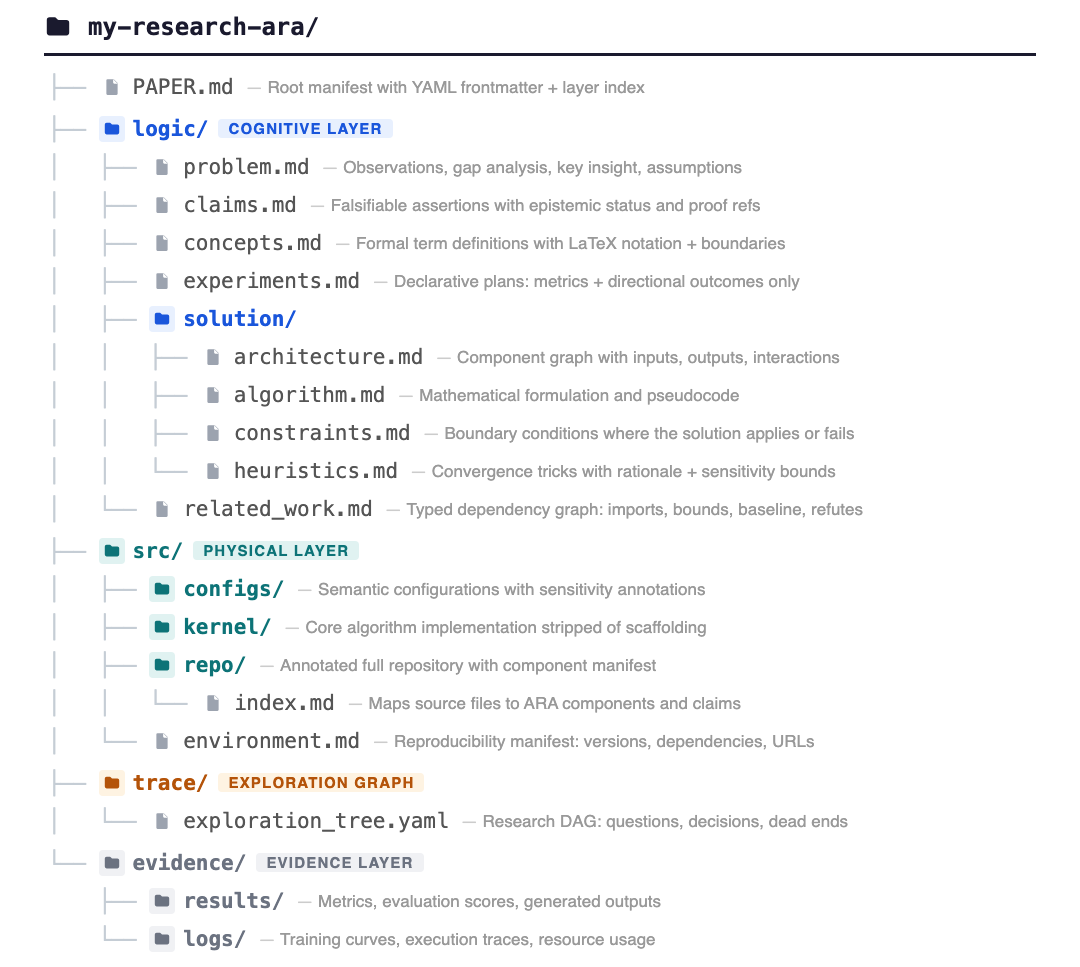
\includegraphics[keepaspectratio]{figures/fig_ara_directory_annotated.png}}

}

\caption{\label{fig-ara-structure}Ara
目录结构。每个文件的角色以内联注释标注；层级徽章标出四个顶层分区。跨层的\emph{取证绑定}将
\passthrough{\lstinline!/logic!} 中的论断链接至
\passthrough{\lstinline!/evidence!} 中的证据和
\passthrough{\lstinline!/src!} 中的代码。完整模式见附录
\ref{sec-app-schema}；设计理由见附录 \ref{sec-app-protocol-details}。}

\end{figure}%

\subsection{设计理念}\label{sec-philosophy}

\textsc{Ara}
协议植根于唯一原则：\textbf{知识重于叙事}------研究过程中产生的有组织、不断演进的知识是第一位的科学对象；叙事性论文只是其编译视图。

\paragraph{结构化的知识容器。}\label{ux7ed3ux6784ux5316ux7684ux77e5ux8bc6ux5bb9ux5668}

一个智能体与某个研究项目交互时，会提出四类结构上截然不同的问题：这项工作\emph{为什么}有效（科学推理），它是\emph{如何}实现的（可执行代码），沿途\emph{尝试了什么}（探索轨迹），以及\emph{数据是什么}（原始经验证据）。
一篇叙事性论文迫使智能体从同一种线性散文中提取这四类答案，然而这些知识类型在结构上存在内在冲突：推理需要稳定、可引用的单元，而代码持续迭代；探索历史本质上是分支结构的，而叙事强制线性；证据需要机器精度的数值，而散文会约简和转述。
将它们压缩到单一文档中不仅是次优的，更是\emph{有损的}：一旦扁平化为叙事，原始结构便无法恢复。
\textsc{Ara}
通过在智能体原生的文件系统结构中，将每种知识类型物化为其专属的层级（图
Figure~\ref{fig-ara-structure}），从而消除这种损耗：这些目录是纯文本、可独立查询的，智能体能够使用标准工具调用进行导航、阅读和操作，而无需解析散文或逆向工程代码仓库。
由于智能体上下文窗口是共享且有限的资源，该结构进一步支持\emph{渐进式披露}：智能体仅加载与当前任务相关的层级和文件，避免不必要的上下文污染。

下面四个层级是对第 Section~\ref{sec-intro}
节引入的叙事税和工程税的结构性回应：探索图谱复原了被叙事折叠的分支轨迹；认知层与物理层通过取证链接相互绑定，弥合了概念性描述与可执行规约之间的鸿沟。
在每个层级内部，构件文本最大化每词元的信息密度：去除主观修饰语、模糊限定和叙事连接词，需要判断的陈述携带的是溯源信息而非修辞渲染。

\begin{figure}[!t]

\centering{

\pandocbounded{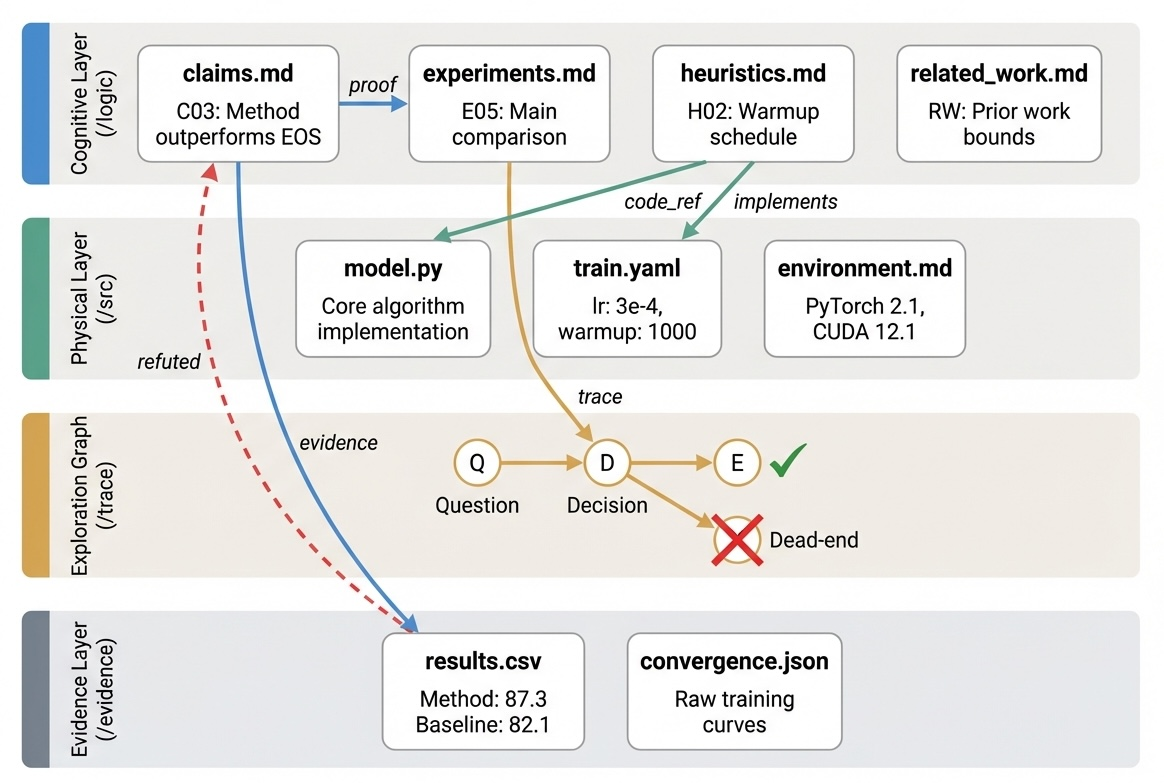
\includegraphics[keepaspectratio]{figures/fig_cross_layer_v2_attempt1.png}}

}

\caption{\label{fig-exploration-graph}真实 Ara
的跨层结构。\passthrough{\lstinline!/logic!} 中的论断通过取证绑定链接至
\passthrough{\lstinline!/src!} 中的代码和
\passthrough{\lstinline!/evidence!}
中的证据。探索图谱（底部中央）捕获研究 DAG，其中死胡同节点（标记为
\(\times\)）保留了失败模式和教训。}

\end{figure}%

\subsection{\texorpdfstring{\textsc{Ara} 架构}{ 架构}}\label{sec-layers}

一个智能体与某个研究构件交互时，有四种基本需求：\emph{理解}贡献、\emph{复现}贡献、\emph{从过程中学习}，以及基于原始证据\emph{验证}论断。
\textsc{Ara} 将每种需求物化为一层专用层级（图
Figure~\ref{fig-ara-structure}），并以清单文件
\passthrough{\lstinline!PAPER.md!} 为根，其 YAML
前置元数据和层级索引使智能体能在 \({\sim}500\) 词元内判定相关性（附录
\ref{sec-app-schema}）。 此分解的制定参考了基于 PaperBench
评分标准提炼的十类复现关键信息分类体系（附录 \ref{sec-app-taxonomy}）。

\paragraph{\texorpdfstring{认知层（\texttt{/logic}）。}{认知层（/logic）。}}\label{ux8ba4ux77e5ux5c42logic}

智能体\emph{首先}阅读 \passthrough{\lstinline!/logic!}
以理解\emph{做了什么以及为什么}：\passthrough{\lstinline!problem.md!}
定义问题空白和核心洞察，\passthrough{\lstinline!solution/!}
指定架构、算法和收敛关键的启发式规则，\passthrough{\lstinline!claims.md!}
提炼可证伪的断言并配以显式证明指针，\passthrough{\lstinline!experiments.md!}
声明验证计划。 \passthrough{\lstinline!related\_work.md!}
用智能体可操作的\emph{类型化依赖}取代被动引用：\passthrough{\lstinline!imports!}
注入先验定义，\passthrough{\lstinline!bounds!}
将约束传播到超参数搜索，\passthrough{\lstinline!baseline!}
条目支持自动回归检测，从而将文献综述转变为机器可执行的依赖图。

\paragraph{\texorpdfstring{物理层（\texttt{/src}）。}{物理层（/src）。}}\label{ux7269ux7406ux5c42src}

存放\emph{如何实现}------针对贡献类型校准的可执行代码。
算法性贡献使用\emph{内核模式}：仅包含带有类型化 I/O
签名的核心模块，通常比完整仓库小一到两个数量级，从而编码智能体能够按需重新生成环境原生的样板代码。
系统性贡献（CUDA
内核、分布式训练、系统架构）使用\emph{仓库模式}：保留完整实现，但通过
\passthrough{\lstinline!index.md!}
清单加以标注，将每个源文件映射到其所实现的 \textsc{Ara} 组件。
\passthrough{\lstinline!configs/!}
为每个超参数标注理由和搜索范围；\passthrough{\lstinline!environment.md!}
锁定依赖、硬件和随机种子（模式规约、取证绑定及详细理由见附录
\ref{sec-app-src-modes}）。

\paragraph{\texorpdfstring{探索图谱（\texttt{/trace}）。}{探索图谱（/trace）。}}\label{ux63a2ux7d22ux56feux8c31trace}

\passthrough{\lstinline!exploration\_tree.yaml!}
将完整的研究有向无环图（DAG）存储为嵌套 YAML
树，包含五种类型化节点------\passthrough{\lstinline!question!}、\passthrough{\lstinline!decision!}、\passthrough{\lstinline!experiment!}、\passthrough{\lstinline!dead\_end!}、\passthrough{\lstinline!pivot!}------其中嵌套编码父\(\to\)子边，而
\passthrough{\lstinline!also\_depends\_on!} 字段捕获收敛点。
该格式充当``研究的 git
log''：智能体可直接遍历分支，而叙事性论文所丢弃的死胡同节点，则保留了假设、失败模式和教训（图
Figure~\ref{fig-exploration-graph}）。

\paragraph{\texorpdfstring{证据层（\texttt{/evidence}）。}{证据层（/evidence）。}}\label{ux8bc1ux636eux5c42evidence}

支撑每个论断的原始输出：\passthrough{\lstinline!results/!}
包含机器可读的指标表和生成数据，附有精确取值和来源注释；\passthrough{\lstinline!logs/!}
捕获训练曲线、资源使用和诊断信息。
它\emph{仅}持有输出，从而每个论断的证明链沿
\passthrough{\lstinline!claims.md!} \(\to\)
\passthrough{\lstinline!experiments.md!} \(\to\)
\passthrough{\lstinline!/evidence/!} 流动。

\paragraph{隐去真实值实现层级化访问控制。}\label{ux9690ux53bbux771fux5b9eux503cux5b9eux73b0ux5c42ux7ea7ux5316ux8bbfux95eeux63a7ux5236}

实验\emph{逻辑}（验证什么）位于
\passthrough{\lstinline!/logic!}；实验\emph{数据}（确切结果）仅位于
\passthrough{\lstinline!/evidence!}。
可以在隐去证据层的情况下向验证智能体授予代码内核和算法描述，从而防止其通过复制预期值来伪造结果。
这种分离还使每个 \textsc{Ara} 成为一个即开即用的训练环境：任务位于
\passthrough{\lstinline!/logic/experiments.md!}，奖励位于
\passthrough{\lstinline!/evidence/!}，而偏好信号则蕴含于
\passthrough{\lstinline!/trace/!} 中记录的每一次接受、拒绝和修订之中。

我们认为，当一个\emph{能力足够}的编码智能体能够纯粹基于 \textsc{Ara}
\emph{零样本}地复现核心论断时------无需人工干预，也不依赖构件本身之外的任何外部上下文------则该
\textsc{Ara}
是充分的。因此，充分性是一个相对于能力的准则：它衡量的是构件是否\emph{包含}复现其论断所需的信息，而非当下的任何智能体是否能够充分利用它。在智能体能力的极限处，一个完整的
\textsc{Ara}
按定义即是可复现的，因此今天撰写的构件在智能体进化后仍然有效。

\FloatBarrier

\section{实时研究管理器}\label{sec-live-pm}

前一节定义了 \textsc{Ara} 协议：一种结构化的研究知识目标格式。
一个自然的问题随之而来：\emph{谁来填充它？}
要求研究者手工编写结构化文件，不过是用一种文档负担替代另一种，恰好否定了协议试图消除的税收本身。

关键观察是，在 AI
原生研究中，完整的研究轨迹------每一次设计选择、每一次失败实验、每一条来之不易的启发式规则------已经作为机器可读的文本存在于研究者与智能体之间的对话中。
实时研究管理器将这些潜在信号结晶化为一个活态的 \textsc{Ara}
构件，该构件在后台有机地累积，对研究者而言零文档开销。\footnote{\url{https://github.com/AmberLJC/Agent-Native-Research-Artifact}}
我们从 AI
原生范式中推导出设计原则（\S\ref{sec-design-principles}），并给出实现这些原则的系统（\S\ref{sec-lrm-design}；图
Figure~\ref{fig-lrm-overview}）。

\begin{figure}[!t]

\centering{

\pandocbounded{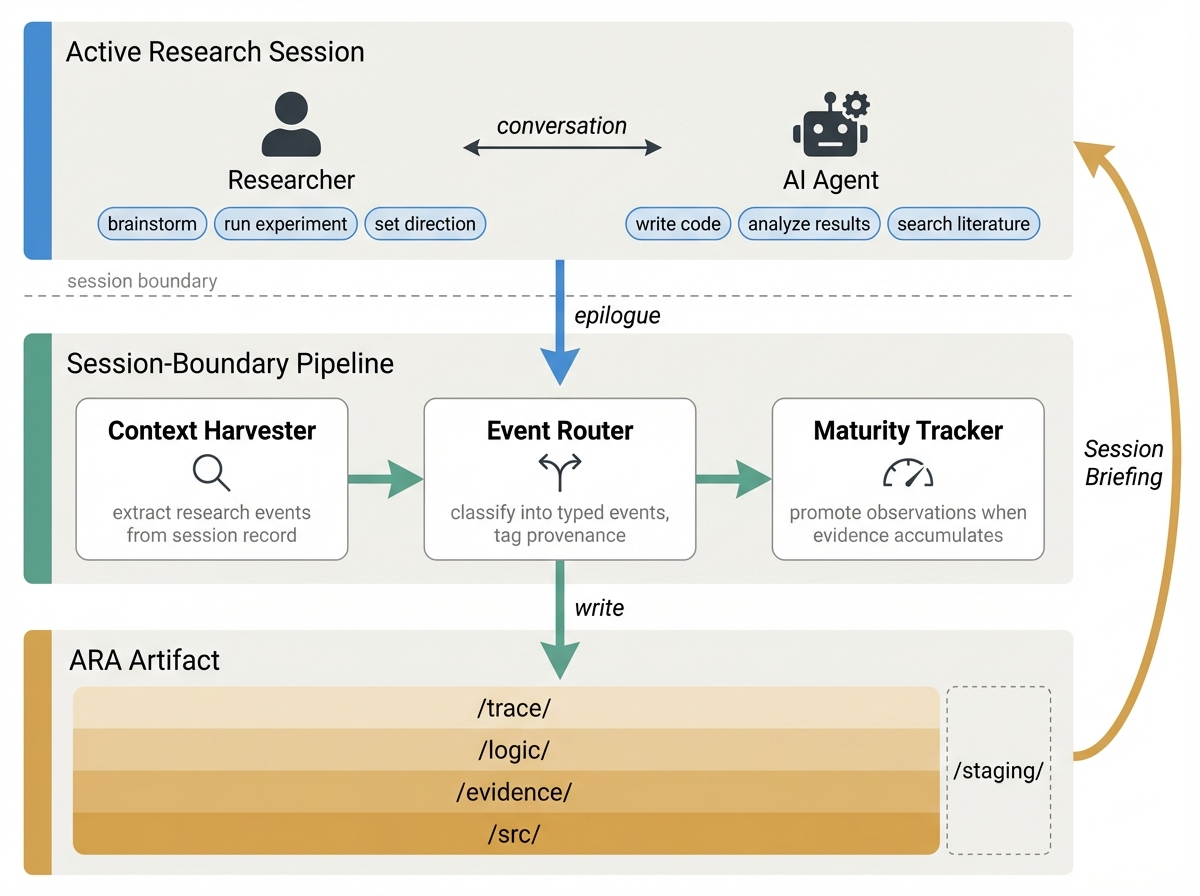
\includegraphics[keepaspectratio]{figures/fig_lrm_lifecycle_v5_attempt2.png}}

}

\caption{\label{fig-lrm-overview}实时研究管理器在会话边界处运行：一个三阶段流水线（上下文采集器
\(\to\) 事件路由器 \(\to\)
成熟度追踪器）将每次研究者--智能体会话提炼为类型化事件，并随时间推移在各
Ara 层级中累积。}

\end{figure}%

\subsection{设计原则}\label{sec-design-principles}

\paragraph{AI 原生研究。}\label{ai-ux539fux751fux7814ux7a76}

计算机科学研究正日益\emph{AI
原生}化：研究者与通用编码智能体在整个研究生命周期中协作。
单次对话循环可能横跨提出假设、综述相关工作、编写和调试实验代码、分析结果以及撰写论文------研究者提供方向，智能体执行，该循环日复一日、周复一周地重复。
这一范式转变具有一个结构性后果：有史以来第一次，研究过程\emph{生而数字化、生而文本化}。
每一条指令、每一个中间结果、每一次设计选择、每一个被放弃的方向，都已经以机器可读的文本形式存在------这是完整研究记录的原材料，仅缺一个让其自然结晶的系统。
此前保存过程知识的努力------负面结果期刊
\citep{matosin2014negativity}、注册报告
\citep{chambers2013registered}------之所以失败，是因为文档化仍然是研究者的一项独立的、得不到回报的负担。
AI
原生研究消解了这一障碍：过程轨迹不是额外的交付物，而是研究本身的\emph{副产品}，在每一次研究者--智能体会话中自动生成。
换言之，我们正处于科学史上前所未有的时刻：全面的研究过程捕获首次在边际成本可忽略不计的条件下成为可行。

这一观察催生了实时研究管理器：如果研究轨迹已在对话中被捕获，那么一个后台系统就可以将其提炼为结构化的
\textsc{Ara}，而无需研究者额外记录任何内容。
我们由此范式推导出三项设计原则。

\begin{enumerate}
\def\labelenumi{\arabic{enumi}.}
\tightlist
\item
  \textbf{静默、框架无关的集成}：管理器是一份自然语言规约，可由任何编码智能体加载，无需自定义
  SDK。它作为后台进程静默运行，在不干扰研究者的情况下自动采集研究痕迹。
\item
  \textbf{忠实的知识溯源}：每个事件均标注来源（\passthrough{\lstinline!user!}、\passthrough{\lstinline!ai-suggested!}、\passthrough{\lstinline!ai-executed!}、\passthrough{\lstinline!user-revised!}），以保留认识论起源。原始观察先被暂存而非强行归类，随着证据累积逐步成熟为类型化事件，从而下游消费者不仅能重建\emph{得出了什么结论}，还能重建\emph{为何得出此结论}。
\item
  \textbf{全面的轨迹捕获}：完整的分支研究过程，包括死胡同和转向，均被记录，并在捕获时建立跨层绑定。构件受版本控制，因此每个里程碑产生一个可导航的快照，而回溯性修订是一等操作，而非破坏性覆写。
\end{enumerate}

每条原则的完整理由见附录 \ref{sec-app-lrm-principles}。

\subsection{系统设计}\label{sec-lrm-design}

\paragraph{概述。}\label{ux6982ux8ff0}

我们将实时研究管理器实现为一个\emph{智能体技能}
\citep{agentskills2025}：一份轻量级的自然语言规约，当加载到通用编码智能体的上下文窗口中时，将其转变为一个领域专用的智能体（\textbf{P1}）。
一个技能不需要自定义 SDK
或基础设施；它简单地将智能体已具备的工具（文件读取、写入、编辑、shell
执行）与 \textsc{Ara}
模式的领域知识进行组合，且构件质量会随底层语言模型的进步而自动提升。
该技能是开源的，详见
\url{https://github.com/AmberLJC/Agent-Native-Research-Artifact}。

管理器在活跃研究期间保持静默，然后在每次对话结束时运行一个三阶段回溯流水线（\textbf{P1}；图
Figure~\ref{fig-lrm-overview}）。
\textbf{上下文采集器}扫描会话记录------对话历史、工具输出、实验结果和代码差异------以提取具有研究意义的事件。
\textbf{事件路由器}对每个事件进行分类，标注来源，并将其写入相应的
\textsc{Ara} 层级。
\textbf{成熟度追踪器}审查暂存区，将已积累足够证据的观察提升为正式条目，并标记过时或冲突项。
在下一会话开始时，管理器读回构件，呈现一份结构化的简报，从而闭合循环。
本小节余下部分将详述每个阶段以及将它们联结在一起的跨会话机制。

\paragraph{上下文采集与事件路由。}\label{ux4e0aux4e0bux6587ux91c7ux96c6ux4e0eux4e8bux4ef6ux8defux7531}

上下文采集器扫描完整的会话记录，识别两类具有研究意义的活动：AI
智能体已执行的操作（如实验运行、代码变更、文献搜索）以及研究者已表达或确认的方向（如待测试的假设、设计选择、被放弃的方案）。
事件路由器随后将每个提取出的事件归入七种类型之一（表
\ref{tbl-event-types}），并标注来源（\textbf{P2}）------\passthrough{\lstinline!user!}、\passthrough{\lstinline!ai-suggested!}、\passthrough{\lstinline!ai-executed!}
或 \passthrough{\lstinline!user-revised!}。 一个
\passthrough{\lstinline!ai-suggested!}
事件在研究者显式确认之前绝不自升级，从而保持构件的知识完整性。
事件载荷遵循协议的事实密度要求（\S\ref{sec-philosophy}）：对话散文在提交到构件之前被提炼为电报式的、量化的语言。
每个类型化事件被写入相应的 \textsc{Ara}
层级：轨迹事件（决策、实验、死胡同、转向）追加到探索图谱（\passthrough{\lstinline!/trace/!}），构建一条忠实的、按时序排列的研究轨迹记录，包括那些被尝试和放弃的方向（\textbf{P3}）；论断和启发式规则进入认知层（\passthrough{\lstinline!/logic/!}）；而难以归类的事件则暂存于
\passthrough{\lstinline!/staging/!} 中，等待后续提升。

\begin{table}[htbp]
\centering
\begin{tabular}{llll}
\toprule
\textbf{事件类型} & \textbf{结构化载荷} & \textbf{事件类型} & \textbf{结构化载荷} \\
\midrule
\texttt{决策} & 选择、备选项、依据 & \texttt{论断} & 陈述、可证伪条件 \\
\texttt{实验} & 量化指标、论断链接 & \texttt{启发式规则} & 技巧、敏感性、边界 \\
\texttt{死胡同} & 假设、失败模式、教训 & \texttt{观察} & 原始发现，待分类 \\
\texttt{转向} & 触发因素、理由 &  &  \\
\bottomrule
\end{tabular}
\caption{研究事件类型及其结构化载荷。}
\end{table}

\paragraph{渐进式结晶化。}\label{ux6e10ux8fdbux5f0fux7ed3ux6676ux5316}

构件构建在两个时间尺度上进行（\textbf{P2}）。
\emph{持续地}，在每次会话边界处，管理器将轨迹事件追加到探索图谱中，记录研究者如何在开放式研究空间中导航。
\emph{周期性地}，当达到一个重大里程碑------假设被证实或证伪、工作原型完成、关键设计选择最终确定------成熟度追踪器将累积的观察\emph{结晶化}为构件中更结构化的层级。
原始观察成熟为认知层（\passthrough{\lstinline!/logic/!}）中的正式论断，工作代码被记录到物理层（\passthrough{\lstinline!/src/!}），概念被添加到知识索引中。
这种两阶段节奏反映了研究理解实际发展的方式：洞察始于零散的观察，而强制过早的结构化会扭曲记录。
管理器将尚不可归类的内容暂存起来，仅当会话记录中的\emph{闭合信号}------话题放弃、研究者显式确认、关联实验的经验性解决，或构件级别的提交------表明该观察已被视为确定时，才进行结晶化（附录
\ref{sec-app-lrm-maturity}）。
当某个转向使先前的设计选择失效时，管理器会传播该变更：更新受影响构件条目（论断、启发式规则或配置）以反映新的方向，而探索图谱保留原始理由和修订原因。
由于构件受版本控制，每次里程碑结晶化都会产生一次提交，使项目拥有其智力演进的可导航历史，正如
GitHub 为代码所做的那样。

\paragraph{跨会话连续性。}\label{ux8de8ux4f1aux8bddux8fdeux7eedux6027}

管理器是无状态的；构件本身承载了跨会话的记忆。在会话结束时，它写入一份简短的会话记录（已捕获的事件、涉及到的论断、开放议题），并追加到运行中的会话索引中。下一次会话读取该索引以及当前的论断和暂存的观察，仅在与当前任务相关时才调出相应内容，而非以研究者并未要求的正式简报打头阵（附录
\ref{sec-app-lrm-continuity}）。

\section{\texorpdfstring{\textsc{Ara}
编译器}{ 编译器}}\label{sec-ingestor}

原生智能体路径（\ref{sec-live-pm}）通过在研究过程中捕获涌现的知识，生成最高保真度的
\textsc{Ara}。 然而，科学记录中包含了数以百万计的、从未被结构化的遗留
PDF，而原生智能体路径无法回溯至这些历史文献。 除 PDF
本身之外，研究知识还分散在各种补充性来源中：GitHub
仓库编码了正文中省略的实现决策，专家策划的评估量规编码了领域实践者所认定的核心论断，记录下来的实验轨迹则保存了论文系统性地加以抑制的失败模式。
为了弥合这一鸿沟，我们提出了 \textbf{\textsc{Ara}
编译器}，这是一项智能体技能，能将任意的遗留研究来源组合转换为一个完整的
\textsc{Ara}。\footnote{\url{https://github.com/AmberLJC/Agent-Native-Research-Artifact}}
质量通过两个阶段来保证。在编译过程中，编译器仅使用 ARA
认证第一级作为环内验证信号。编译完成后，成品构件进入下游认证流水线，由第二至第三级评估其论证性支撑和经验性可复现性（\ref{sec-liveness}）。

\begin{figure}[!t]

\centering{

\pandocbounded{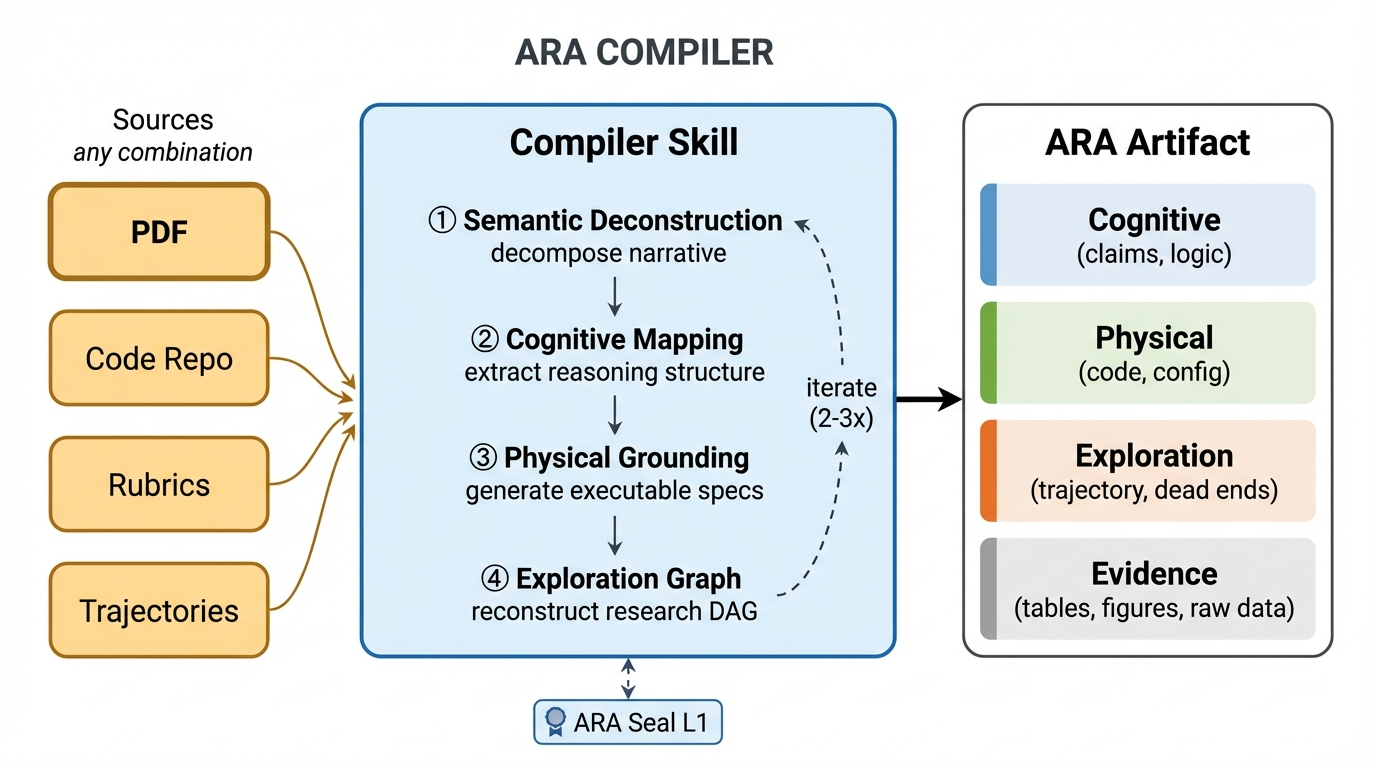
\includegraphics[keepaspectratio]{figures/fig_compiler_v2.png}}

}

\caption{\label{fig-ingestor-pipeline}Ara
编译器接受任意的研究来源组合，引导编码智能体通过四个阶段的自顶向下构件编译，并与环内
ARA 认证第一级验证迭代 2--3\(\times\)，直至输出符合协议规范。}

\end{figure}%

\subsection{设计原则}\label{sec-ingestor-principles}

\paragraph{通用输入，规范输出。}\label{ux901aux7528ux8f93ux5165ux89c4ux8303ux8f93ux51fa}

编译器是多对一的：它接受任意组合的
PDF、代码仓库、数据集、人类策划的量规（例如 PaperBench
\citep{starace2025paperbench} 的论断分解）以及实验轨迹日志（例如
RE-Bench \citep{wijk2025rebench}
中记录论文所省略之失败的追踪数据），且始终输出一个符合
Section~\ref{sec-protocol} 规范的单一 \textsc{Ara}。
降级是优雅的：仅凭一个 PDF
就能生成一个具有桩级物理层的有效构件；更丰富的输入则能逐步填充更完整的层。

\paragraph{高保真保存。}\label{ux9ad8ux4fddux771fux4fddux5b58}

叙事性论文进行压缩和筛选；编译器则进行解压缩和恢复。
来源中的每一个数值结果、超参数、架构细节和负面发现都必须出现在构件的\emph{某处}，任何
PDF 中可获取但 \textsc{Ara} 中缺失的信息都构成编译失败（在
\ref{sec-eval-understanding} 中进行评估）。
保存是忠实于来源的；\emph{丰富化}（Section~\ref{sec-collective}）则单独发掘出任何单一来源都无法表达的跨构件模式。

\paragraph{知识谱系，而非扁平提取。}\label{ux77e5ux8bc6ux8c31ux7cfbux800cux975eux6241ux5e73ux63d0ux53d6}

叙事性编译会破坏连接论断与实验、实验与证据、证据与代码的\emph{溯源链}。
纯文本抽取能恢复内容，但无法恢复这些连接：将 PDF 解析为 Markdown
会填充四个目录，却使它们在结构上彼此孤立。
编译器执行\emph{取证重建}，从那些仅隐含存在谱系的来源（散落在正文、图注、附录表格和代码注释中）中恢复跨层取证绑定（Section~\ref{sec-layers}），从而使智能体能够将任意论断向下追溯至代码，或向上追溯至其假设。
编译的核心问题在于恢复这一谱系，而非填充各层。

\subsection{编译器实现}\label{sec-ingestion-skill}

针对叙事性 PDF
实现这些原则，需要具体的机制来解决正文如何模糊化结构、谱系和来源多样性的特定方式。
编译器被实现为单一智能体技能（图
Figure~\ref{fig-ingestor-pipeline}），引导编码智能体完成从遗留来源到
\textsc{Ara} 格式的转换。 技能提示词编码了完整的 \textsc{Ara}
模式、字段级需求以及结构化的生成协议。
我们在下文描述关键要素；完整的技能规范复现于附录
\ref{sec-app-ingestor-prompt}。

\paragraph{自顶向下生成。}\label{ux81eaux9876ux5411ux4e0bux751fux6210}

该技能指示智能体\emph{自顶向下}地构建构件，如同研究者向新合作者解释其工作的方式：先讲高层概念，再讲细节，最后讲实现。
具体而言，智能体经历四个阶段。
\emph{语义解构}剥离叙事框架，以暴露原始研究内容（公式形式、配置、结果、依赖关系、失败方法），并将其改写为事实密集的电报式形式，从而在来源层面消除叙事税（Storytelling
Tax）。 \emph{认知映射}填充
\passthrough{\lstinline!/logic!}：动机链（观察 \(\to\) 缺口 \(\to\)
洞察）、带有证明指针的可证伪论断、形式化概念以及解决方案结构，且每个论断都关联至验证它的实验。
\emph{物理落地}生成
\passthrough{\lstinline!/src!}：带注释的配置、类型化代码桩以及环境清单；当有代码仓库可用时，桩被替换为实际实现，智能体执行\emph{代码-论文对齐}，将代码库与论断进行交叉比对，以显露出隐性知识------隐含假设、无文档记录的技巧、额外参数
\citep{li2026tacit}------并将其作为溯源标记的启发式规则写回
\passthrough{\lstinline!/logic!}。 \emph{探索图谱提取}将研究 DAG
重建为嵌套的 YAML 树，其中死胡同叶节点记录了假设、失败模式和教训。
这种顺序确保每一层都受其上一层的指导：认知结构引导物理层生成，而探索图谱为两者提供上下文。

\paragraph{通过验证反馈的迭代精化。}\label{ux901aux8fc7ux9a8cux8bc1ux53cdux9988ux7684ux8fedux4ee3ux7cbeux5316}

初始生成后，ARA
认证第一级检查（\ref{sec-liveness}）------包括模式一致性、跨层引用解析、必填字段完整性------在同一智能体会话中运行，将失败返回为结构化的诊断信息，驱动针对性修复。
这种生成\(\,\to\,\)验证\(\,\to\,\)修复的循环通常在 2--3
轮中收敛，将第一级转变为可操作的反馈，而非事后报告。

\paragraph{来源感知的丰富化。}\label{sec-collective}

辅助性来源被路由至其最直接填充的层：代码仓库将
\passthrough{\lstinline!/src!}
中的桩替换为经过验证的实现；评估量规通过专家验证的论断分解来锚定
\passthrough{\lstinline!/logic!}；轨迹日志则用 PDF
所省略的死胡同节点来播种 \passthrough{\lstinline!/trace!}。
当已有先前编译的 \textsc{Ara}
库可用时，编译器进一步执行\emph{集体推断}：从同领域构件中检索启发式规则和配置，标记出当前论文遗漏的常见模式，并将其添加为标记为
\passthrough{\lstinline!collective\_inference!}
的候选启发式规则，使下游智能体能够区分陈述性知识与推断性知识。

\FloatBarrier

\section{\texorpdfstring{\textsc{Ara}
验证与评审}{ 验证与评审}}\label{sec-review-system}

专家人类注意力是科学评价中最稀缺的资源。
顶级会议的审稿负载增长速度快于审稿人队伍的增长
\citep{aczel2021billiondollar}，而审稿人的精力日益被机械性验证（``代码能运行吗？''、``表
3 支持论断 2 吗？''）所消耗，而非用于只有领域专家才能提供的实质性判断。

因为 \textsc{Ara} 提交\emph{就是}一个结构化的、机器可执行的构件，PDF
审稿主观检查的结构性属性变得客观可验证：模式一致性和跨层引用完整性要么确定性地通过，要么确定性地失败。
更高阶的属性------信息完整性和核心论断的方向性可复现性------变得\emph{机器可评估}：自动化检查提供概率性证据，为人类审稿人提供信息依据，而非取代他们。
这种分离将专家注意力从机械性检查重新导向只有人类才能提供的实质性判断：重要性、新颖性与品位。
我们将\textbf{ARA
认证}定义为一个具有三个递增级别的机器可验证凭证（\S\ref{sec-liveness}，图
Figure~\ref{fig-ara-seal}），并描述了一个三阶段评审流水线（图
Figure~\ref{fig-review-pipeline}），该流水线利用这些级别将自动化验证与人类判断分离开来。

\subsection{设计原则}\label{sec-review-principles}

我们在下文中推导出两条设计原则；跨构件审稿------即通过智能体对智能体的
ARA 比较------只有在语料库达到临界规模时才有意义，相关讨论见
\S\ref{sec-discussion}。

\paragraph{P1.
自动化机械性工作；将判断留给人类。}\label{p1.-ux81eaux52a8ux5316ux673aux68b0ux6027ux5de5ux4f5cux5c06ux5224ux65adux7559ux7ed9ux4ebaux7c7b}

结构有效性、内部一致性和论断可复现性是客观属性，要么通过，要么不通过；而重要性、新颖性和品位则需要领域专业知识。
评审系统永远不应要求人类去验证实验 E03 是否与论断 C02
匹配------当机器可以在数秒内完成时；在构件到达人类审稿人\emph{之前}解决所有机器可检查的问题，确保专家注意力仅用于真正需要它的那些问题。

\paragraph{P2.
可复现性作为基础要求。}\label{p2.-ux53efux590dux73b0ux6027ux4f5cux4e3aux57faux7840ux8981ux6c42}

``代码按需提供''名义上满足了当今的可复现性门槛；在 \textsc{Ara}
原生系统中，可复现性是构件本身的\emph{机器验证属性}。 通过 ARA
认证第一级（结构完整性）是投稿要求，第二级（论证严谨性）在会议投入算力进行第三级（执行可复现性）之前产生结构化审读意见，而第三级的结果随后会附加到每一份评审中。
未能通过结构检查、或经第二级审读后其论断仍明显缺乏支撑的构件，不会进入人类审稿阶段。

\subsection{ARA 认证：机器可验证的研究凭证}\label{sec-liveness}

\begin{figure}[!t]

\centering{

\pandocbounded{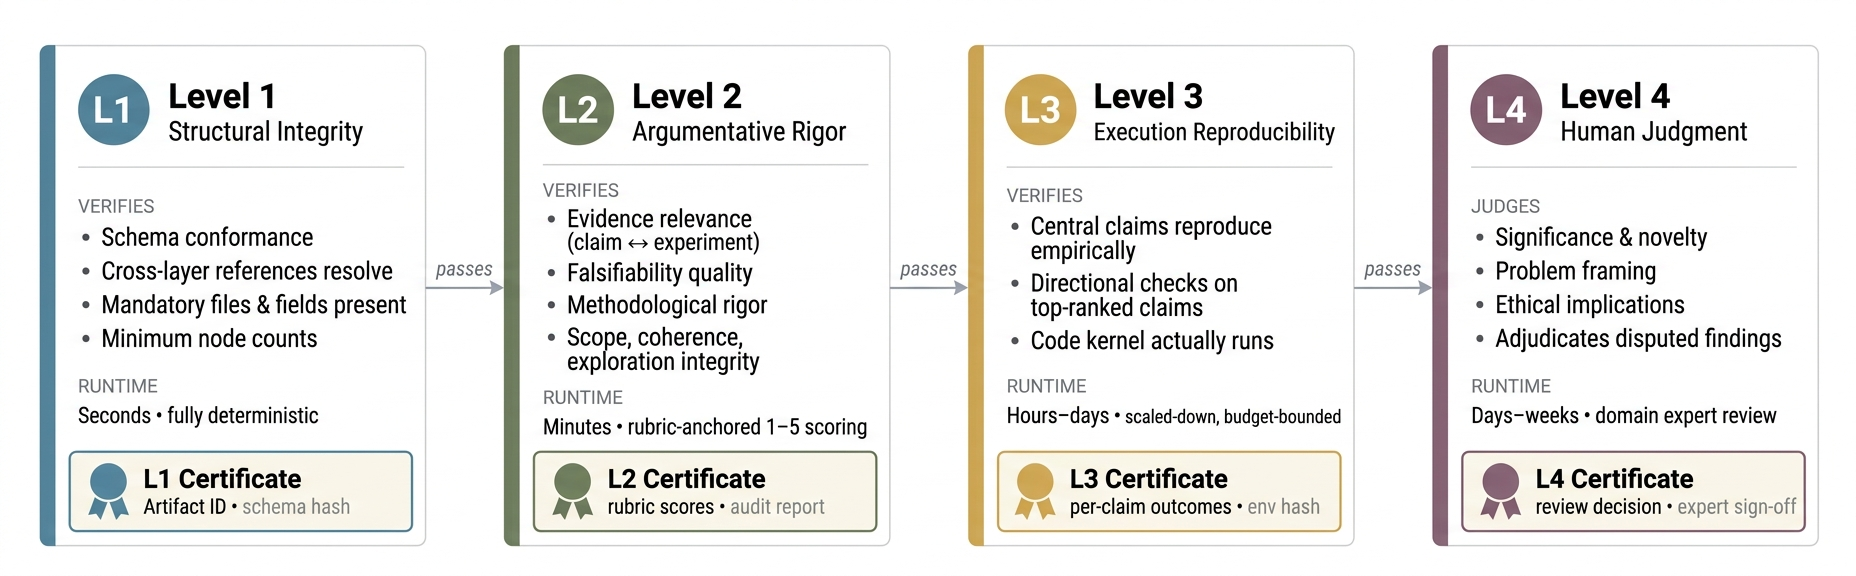
\includegraphics[keepaspectratio]{figures/fig_ara_seal.png}}

}

\caption{\label{fig-ara-seal}ARA
认证是一个三级验证凭证。每一级测试构件的一个逐步增强的属性，在成本和广度上逐级提升：结构完整性（数秒，确定性）、论证严谨性（数分钟，基于量规锚定的智能体）以及执行可复现性（数小时至数天，沙箱化的编码智能体）。通过适用的级别后，会颁发一份认证证书，下游智能体在投入算力之前会对其进行检查。}

\end{figure}%

一篇 PDF
论文间接地赢得信任：会议声望、引用数量和作者声誉作为质量的代理指标，但无一能验证工作本身。
因为 \textsc{Ara}
将研究编码为带有显式论断-证据绑定的类型化、机器可遍历的数据，其质量变得\emph{可直接验证}。
ARA 认证将其操作化为一个三级验证协议（图
Figure~\ref{fig-ara-seal}），其中每一级测试一个逐步增强的属性（实现细节见附录
\ref{sec-app-seal-details}）。

\textbf{Level 1 -- 结构完整性}

验证构件格式正确且内部一致：
目录本体存在，所有结构化文件符合其模式（每个论断包含
\passthrough{\lstinline!Statement!}、\passthrough{\lstinline!Status!}、\passthrough{\lstinline!Falsification criteria!}
和 \passthrough{\lstinline!Proof!}；每个启发式规则包含
\passthrough{\lstinline!Rationale!}、\passthrough{\lstinline!Sensitivity!}
和 \passthrough{\lstinline!Bounds!}），
且所有跨层引用均可解析（\passthrough{\lstinline!claims.md!} 中的实验 ID
指向 \passthrough{\lstinline!experiments.md!}
中的有效条目，代码引用追溯至 \passthrough{\lstinline!/src!} 中的实现）。

\textbf{Level 2 -- 论证严谨性}

在不执行任何代码或查询外部来源的前提下，\emph{严谨性审计器}智能体沿六个客观维度评估已通过第一级验证的构件内容是否在认识论上可靠，每个维度按
1 至 5 分的锚定量规进行评分。 三个承重维度为：
\emph{证据相关性}，检查每个论断所引用的实验在类型感知蕴涵下是否实质性地回应了该论断所断言的内容（因果性论断需要隔离消融实验，泛化性论断需要异质测试条件，改进性论断需要基线比较）；
\emph{可证伪性质量}，检查标准是否可操作、非重言式、范围匹配且无需访问专有数据即可独立检验；
以及\emph{方法论严谨性}，涵盖基线充分性、消融覆盖度、统计报告以及指标-论断对齐。
另外三个维度------范围校准、论证连贯性以及探索完整性------定义于附录
\ref{sec-app-seal-eval-l2}。
发现结果按严重程度（\emph{严重}、\emph{重大}、\emph{轻微}、\emph{建议}）、逐字证据引用以及可操作建议进行收集；总体评分由均分和单维度底线综合得出。
每一项检查都归结为构件内容中由量规锚定的属性，因此第二级保持客观；关于重要性、新颖性和品位的判断则留给第三阶段的人类审稿人。
参考严谨性审计器作为智能体技能发布
\citep{agentskills2025}；\footnote{<github.com/AmberLJC/Agent-Native-Research-Artifact>}
完整协议、维度量规以及评分阈值见附录 \ref{sec-app-seal-eval-l2}。

\textbf{Level 3 -- 执行可复现性}

验证构件的核心论断在经验上具有可复现性。
系统按关键性选择论断------包括贡献列表中的论断、锚定最多下游依赖的论断或作者标记的论断------并运行缩减规模的方向性检查（小数据、少量
epoch、玩具配置），以测试所断言的性质是否在定性上成立，而非复现精确数值。
验证智能体与构件的证据层相隔离：它仅接收代码内核和算法描述，绝不接收报告中呈现的数值，以防止通过复制预期结果来进行伪造。
会议设定算力预算；超出预算的论断被标记为\emph{未验证}。
全规模复现（原始数据集、完整训练运行、精确指标恢复）是可选的，通常在接受后或由社区驱动进行；结果将追加至活态认证证书中。

通过适用的级别后，会颁发一份\textbf{认证证书}------一份带签名的记录，包含构件
ID、所达到的验证级别、时间戳、环境哈希值以及逐论断复现结果。
下游智能体在投入算力之前检查此证书，从而避免冗余的重复验证。

\subsection{三阶段评审流水线}\label{ux4e09ux9636ux6bb5ux8bc4ux5ba1ux6d41ux6c34ux7ebf}

\begin{figure}[!t]

\centering{

\pandocbounded{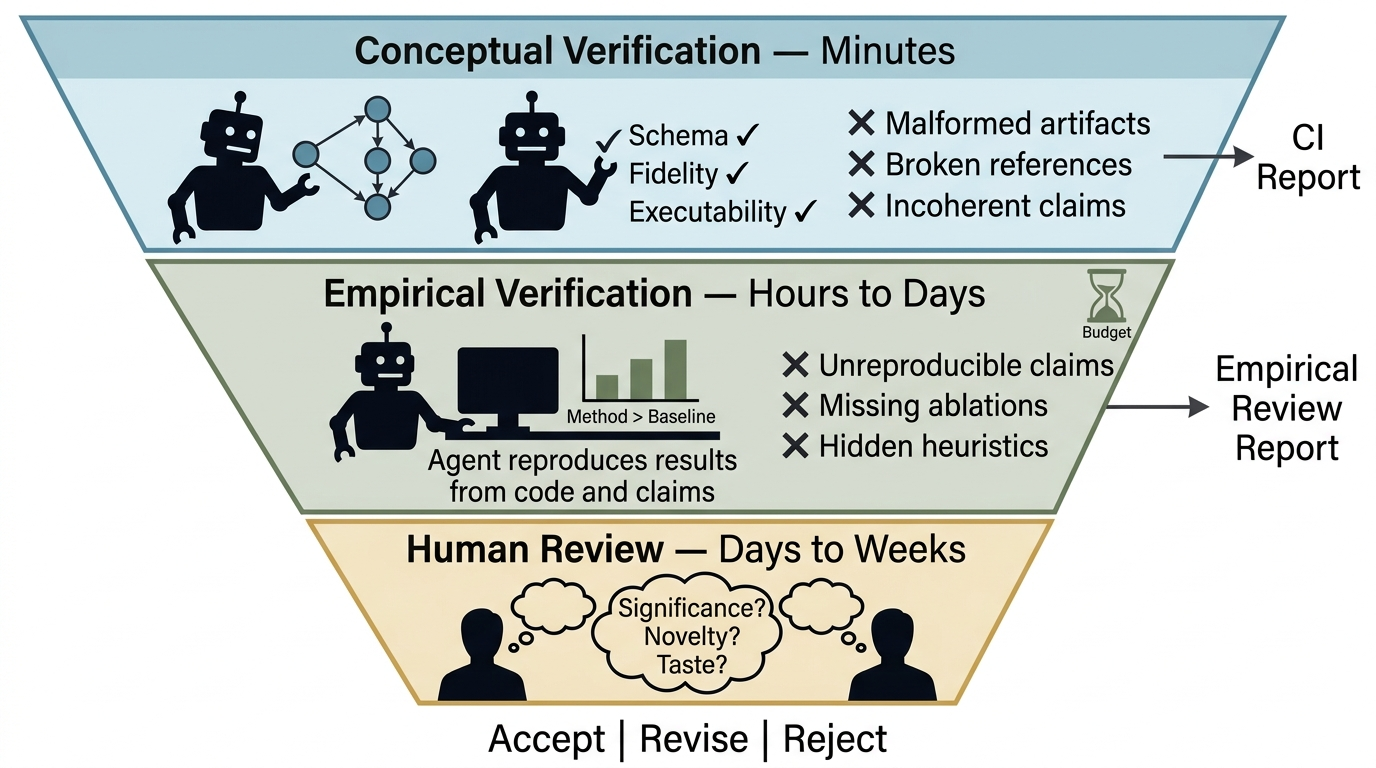
\includegraphics[keepaspectratio]{figures/fig_review_pipeline_v2.png}}

}

\caption{\label{fig-review-pipeline}三阶段 Ara
原生评审流水线。第一至第二阶段调用图 Figure~\ref{fig-ara-seal} 中的 ARA
认证级别，在人类审稿人介入之前解决机械性问题和严谨性问题，将专家注意力重新导向新颖性和重要性。}

\end{figure}%

我们构想了一个模仿 CI/CD 实践的三阶段评审流水线（图
Figure~\ref{fig-review-pipeline}），其中每个阶段为下一阶段把关：概念验证、经验验证和人类判断。

\paragraph{第一阶段：概念验证（数分钟）。}\label{ux7b2cux4e00ux9636ux6bb5ux6982ux5ff5ux9a8cux8bc1ux6570ux5206ux949f}

第一阶段在不运行任何实验的情况下，检查构件是否\emph{格式正确且概念上得到充分支撑}。
自动化检查验证结构完整性（ARA
认证第一级------模式一致性、跨层引用解析、必填字段完整性），严谨性审计器执行第二级论证严谨性，评估主要论断是否范围适当、附带的证据和消融实验是否能为它们提供证明、以及是否有明显的基线、假设或局限性缺失。
第一级检查是机械性和确定性的：\passthrough{\lstinline!claims.md!}
中的每个论断要么链接到一个有效实验，要么没有；启发式规则要么包含敏感度边界，要么缺失。
第二级则产生一份针对特定论断、实验和遗漏的结构化严谨性报告。
该阶段还生成\emph{咨询性诊断信息}，在第三阶段展示给人类审稿人：探索树是否包含死胡同节点（暗示真实的过程文档记录，而非经过净化的线性链条）、相关工作图是否覆盖了明显的基线、以及实验-论断覆盖是否存在缺口。
这些诊断信息提供参考但不设门槛；只有认证检查才是通过/失败的要求。
输出是一份\textbf{CI
报告}加上一份第二级严谨性报告，两者均附于提交中，并对作者和审稿人均可见。
作者在构件进入下一阶段之前，对结构失败和严谨性审读意见进行迭代修正，类似于在代码评审之前修复
lint 错误和设计问题。

\paragraph{第二阶段：经验验证（数小时至数天）。}\label{ux7b2cux4e8cux9636ux6bb5ux7ecfux9a8cux9a8cux8bc1ux6570ux5c0fux65f6ux81f3ux6570ux5929}

一旦构件通过概念评审，第二阶段便测试\emph{所声称的结果是否实际可复现}。
一个 AI 审稿智能体执行 ARA
认证第三级：它按关键性对构件中的论断进行排序------优先考虑贡献列表中的论断以及论断图谱中拥有最多下游依赖的论断------然后在会议指定的算力预算内运行缩减规模的方向性检查（小数据、少量
epoch、玩具配置）。
该智能体与构件的证据层和真实结果相隔离：它仅接收代码内核和算法描述，绝不接收论文中报告的数值，以防止通过复制预期结果来进行伪造。
对于每个被测试的论断，它报告所声称的方向是否成立（例如``方法 A 在指标 M
上优于基线 B''）、所消耗的墙上时钟时间以及任何与预期结果的差异。
超出剩余预算的论断被标记为\emph{未验证}，并附有所需算力的估算。
除复现之外，该智能体还评估实验的全面性：每个设计选择是否都有相应的消融实验？
实验条件是否覆盖了所声称的泛化性，还是结果是从有利设置中精心挑选的？
代码中是否存在未记录在构件认知层中的启发式规则？
输出是一份\textbf{经验评审报告}，记录了哪些论断通过验证、哪些失败、哪些因预算原因被推迟、以及识别出了哪些实验缺口。

\paragraph{第三阶段：人类评审（数天至数周）。}\label{ux7b2cux4e09ux9636ux6bb5ux4ebaux7c7bux8bc4ux5ba1ux6570ux5929ux81f3ux6570ux5468}

人类审稿人收到提交、CI
报告以及经验评审报告，其角色从\emph{验证}------已由第一至第二阶段处理------转变为\emph{判断}。
他们专注于机器无法回答的问题：这一贡献是否重要------它是否解决了一个真正有分量的实际问题？
核心洞见是否真正新颖，还是已知思想的渐进式重组？
这是否是对问题的正确表述，是否存在作者应考虑的更好方法？
其伦理含义和潜在滥用风险是什么？ 当 AI
审稿人的发现有作者提出异议时，人类凭借可供查验的完整审计追踪进行裁决。
人类审稿人以相同的类型化格式撰写结构化评审------将发现链接至特定的
\textsc{Ara} 组件------确保所有反馈均可操作、可追溯。
关键的效率提升：人类不再将时间花费在``你的代码跑不起来''或``表 3 与论断
2 矛盾''上------这些问题在构件到达审稿人之前已经得到解决。

\section{\texorpdfstring{The (Human+AI)\(^{2}\) Research
Network}{The (Human+AI)\^{}\{2\} Research Network}}\label{sec-network}

\begin{figure}[!t]

\centering{

\pandocbounded{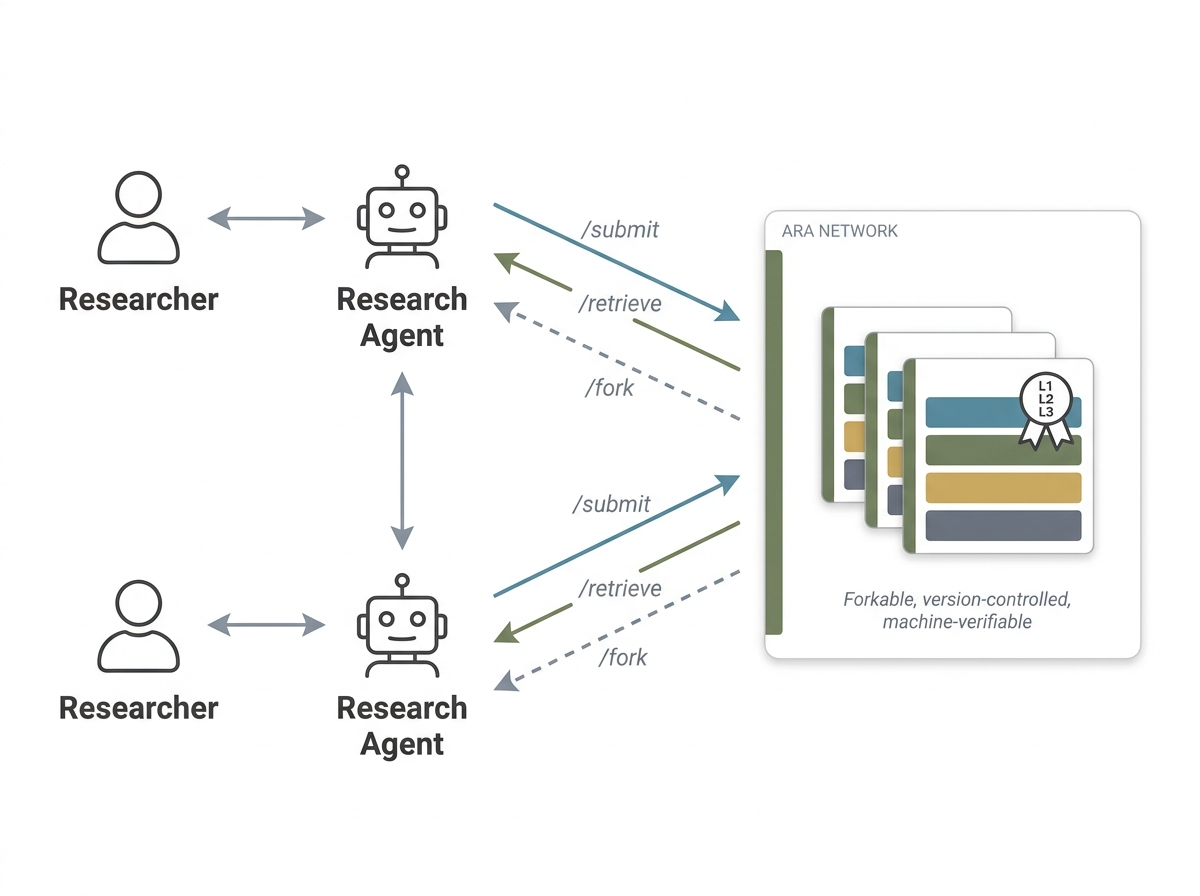
\includegraphics[keepaspectratio]{figures/fig_human_ai_network.png}}

}

\caption{\label{fig-network}(Human+AI)\(^{2}\)
研究网络。每位研究者通过一个研究智能体与共享的 Ara 网络交互，使用
\passthrough{\lstinline!/submit!}、\passthrough{\lstinline!/retrieve!}
和 \passthrough{\lstinline!/fork!} 命令；智能体之间亦可直接协作。}

\end{figure}%

前文各节描述了
\textsc{Ara}-原生技术栈的组成部分：协议（Section~\ref{sec-protocol}）、在开发过程中将工作捕获到构件中的实时研究管理器（\ref{sec-live-pm}）、导入既有文献的编译器（Section~\ref{sec-ingestor}）以及对其进行验证的
Seal
把关审阅流水线（\ref{sec-review-system}）。这些组件组合起来，构成了一个科学交流系统，其主要对象不再是静态文档，而是
\textsc{Ara}
本身：一个统一的规范构件，人类在两端指挥智能体对其进行创作、认证、渲染和扩展。我们将由此形成的结构称为
\textbf{(Human+AI)\(^{2}\) 网络}（图 Figure~\ref{fig-network}）。

在生产者一侧，研究者不再以论文为目标；他们追求问题，而作为产出的论文在此过程中自动积累为
\textsc{Ara}：实时研究管理器在日常工作中将每项决策、每条死胡同和每个已确认的论断纳入构件，编译器按需导入既有来源，在任何里程碑节点，构件经过
Seal
流水线并公开注册，另一个团队可以复刻（fork）一个通过认证的构件，扩展其论断，保留对父构件的署名，并将差异提交以重新审阅。
在消费者一侧，由于 \textsc{Ara}
是规范性的，智能体可按需将其渲染为读者所需的任何界面（论文、视频、幻灯片、交互式演示或基于语境的对话），并根据读者的专业水平、注意力预算和意图进行调整。

由于两端均由智能体中介，且构件是唯一的持久化状态，贡献在构件层面而非句子层面累积：发布成为类似
Git 的操作，审稿人通过他们偏好的界面消费经 Seal 认证的构件，下游智能体将
\textsc{Ara}
作为结构化基线、训练环境或新问题的起点来读取。其结果是一个可查询的科学公地，其中每项贡献都是可执行的差异，理解、复现和扩展的成本随着每个新构件的加入而下降，而非与之对抗上升。\ref{sec-eval}
探讨当今的智能体是否已能在该基座上运行；Section~\ref{sec-discussion}
则勾画了近期、中期和远期的扩展方向。

\FloatBarrier

\section{评估}\label{sec-eval}

\begin{table*}[t]
  \centering
  \small
  \begin{tabular}{@{} p{0.46\linewidth} | p{0.46\linewidth} @{}}
  \toprule
  \textbf{PaperBench}~\citep{starace2025paperbench} & \textbf{RE-Bench}~\citep{wijk2025rebench} \\
  \midrule
  \textbf{论文：} 23篇经同行评审的、横跨多个子领域的机器学习论文 &
  \textbf{任务：} 7个基于明确目标函数的研发爬山任务 \\
  \midrule
  \textbf{规模：} 8,921条由专家编写的评分细则要求 &
  \textbf{规模：} 24,008次智能体运行；46,303个失败episode \\
  \midrule
  \textbf{内容：} PDF + 配套GitHub仓库（23篇中15篇有）；专家评分细则编码了论文中缺失的超参数值、实现技巧和配置信息；失败知识极少在已发表论文中保留 &
  \textbf{内容：} 每个任务的初始代码库；METR MALT转录记录，每次运行保留完整真实智能体的成功与失败轨迹 \\
  \midrule
  \textbf{评分方式：} 专家分层评分细则（是\,/\,部分\,/\,否） &
  \textbf{评分方式：} 自动化连续目标函数；无需人工判断 \\
  \midrule
  \textbf{用于：} 理解（\S\ref{sec-eval-understanding}，A类\,\&\,B类）；复现（\S\ref{sec-eval-reproduction}） &
  \textbf{用于：} 理解（\S\ref{sec-eval-understanding}，C类）；扩展（\S\ref{sec-eval-extension}） \\
  \bottomrule
  \end{tabular}
  \caption{基准测试特征。PaperBench 通过专家评分细则提供配置深度；RE-Bench 通过 MALT 失败轨迹提供探索轨迹深度。这两者正是\ara{}旨在利用的源端富化信息。}
  \label{tab-benchmarks}
\end{table*}

我们在三个研究野心递增的层次上评估\textsc{Ara}：\emph{理解}（智能体能否从构件中提取知识？）、\emph{复现}（智能体能否根据构件执行研究？）和\emph{扩展}（智能体能否借助失败知识更高效地在已有工作之上进行构建？）。每个层次分别隔离了结构化构件相对于以PDF为中心之现状的一项独特优势。我们首先描述评估语料库以及每个\textsc{Ara}是如何从该语料库构建的（\S\ref{sec-eval-data}），然后展示在每个层次上测试\textsc{Ara}的实验（\S\ref{sec-eval-understanding}--\ref{sec-eval-extension}）。所有实验的完整实现细节见附录
\ref{sec-app-eval-details}。

\subsection{数据集与动机}\label{sec-eval-data}

所有三个评估层次都基于同一个比较：在固定智能体、任务和真值的前提下，从一个研究项目可用源材料编译而成的\textsc{Ara}是否优于大多数读者接收到的传统构件------即一篇论文PDF及其配套代码仓库（若存在）？

\paragraph{传统构件中的两个系统性缺口。}\label{ux4f20ux7edfux6784ux4ef6ux4e2dux7684ux4e24ux4e2aux7cfbux7edfux6027ux7f3aux53e3}

这个比较之所以有意义，正是因为传统PDF\(+\)repo会丢失两类\textsc{Ara}能够保留的内容。第一，\emph{配置深度}：已发表论文省略了专家认为复现所必需的超参数、环境规格和实现细节。在PaperBench的8,921条专家复现要求中，源PDF中仅有\textbf{45.4\%}
被完整指定（图 Figure~\ref{fig-info-gap}；完整分类见附录
\ref{sec-app-gap-types}）。第二，\emph{探索深度}：产生最终结果的大部分算力从未进入构件。在24,008次RE-Bench智能体运行中，\textbf{90.2\%}
的美元成本消耗在被已发表构件完全丢弃的失败探索上（附录
\ref{sec-app-exploration-tax}），迫使每个后续智能体重新发现相同的死胡同。我们选用两个基准测试，使每个基准测试作为一等源信息恰好提供传统构件所缺失的内容：PaperBench的专家评分细则弥合了配置缺口；RE-Bench的MALT轨迹弥合了探索缺口（表
\ref{tab-benchmarks}）。这两个基准测试恰好源自计算机科学和机器学习领域，但\textsc{Ara}的设计可扩展到任何其贡献可以表示为代码、配置和有据数据的\emph{数字化}研究，包括计算社会科学、经济学和干实验生物学。其贡献为物理世界干预（湿实验生物学、材料合成）的研究不在本范围内，除非其底层实验记录本身被数字化。

\paragraph{同一研究的两种表示。}\label{ux540cux4e00ux7814ux7a76ux7684ux4e24ux79cdux8868ux793a}

对于每篇论文或每个任务，我们构建同一底层研究的两种表示，并保持其他一切不变。\emph{传统基线}近似大多数读者接收到的内容：对于PaperBench，它是已发表的论文PDF和（若存在，23篇中15篇有）原始GitHub仓库；对于RE-Bench（其任务没有已发表论文），它是一份由LLM合成的、官方参考解决方案的精美论文式撰写文本，搭配官方源码------这是无论文任务中PDF\(+\)repo的最接近类比。\textsc{Ara}则通过\textsc{Ara}编译器（\S\ref{sec-ingestor}）从同一源材料包（PaperBench：PDF\(+\)repo\(+\)专家评分细则；RE-Bench：官方解决方案\(+\)源码\(+\)MALT轨迹）编译而成，并经过ARA认证第1级结构完整性循环（\S\ref{sec-liveness}）的检验；生成--验证--修复迭代在实践中经1--3轮即可收敛。对于扩展实验（\S\ref{sec-eval-extension}），RE-Bench的\textsc{Ara}还额外通过一条专门流水线（附录
\ref{sec-app-extension-pipeline}）生成，该流水线增加了每个MALT运行的提取子智能体和一个超越参考公平性过滤器；输出遵循相同的\textsc{Ara}模式。

\subsection{\texorpdfstring{从\textsc{Ara}中提取知识}{从中提取知识}}\label{sec-eval-understanding}

第一层衡量智能体从每种格式中能够提取什么：\textsc{Ara}是否保留了源PDF和仓库中存在的信息，其结构是否能将源材料中零散或隐含的知识浮现出来？在编译过程中丢失信息的格式无法改善复现或扩展，因此这是每一项下游收益的前提条件。\S\ref{sec-intro}中量化的信息缺口（图
Figure~\ref{fig-info-gap}）表明，结构\emph{能够}恢复PDF未充分指定的细节；本层测试编译器是否真正实现了这一承诺。

\paragraph{实验设置。}\label{ux5b9eux9a8cux8bbeux7f6e}

我们使用450个问题探测每种格式：涵盖30个评估目标（23篇PaperBench论文和7个RE-Bench任务），每个目标15个问题，分为三类。\emph{A类}（每个目标10个，两个基准测试均适用）测试对可从PDF中回答的表面结果、方法和条件的忠实度。\emph{B类}（每篇PaperBench论文5个）测试对超参数、环境规格和预处理细节的配置恢复能力。\emph{C类}（每个RE-Bench任务5个）测试对死胡同、已考虑的替代方案和经验教训的失败知识掌握。为避免问题选择中的来源偏差，我们为每个目标独立生成两个问题池------一个以阅读PDF为种子，一个以阅读\textsc{Ara}为种子------然后合并并去重，使两种格式都无法决定哪些问题被提出（完整模板和金标准评分细则见附录
\ref{sec-app-question-bank}）。每个（目标，格式，问题）三元组作为一个独立的Claude
Sonnet 4.6子智能体分发，拥有全新上下文，每个答案由Claude Opus
4.6裁判根据金标准进行三元评分（1.0 / 0.5 / 0.0）。

\begin{table}[t]
\centering
\small
\begin{tabular}{lc cc cc}
\toprule
& & \multicolumn{2}{c}{\textbf{准确率（\%）}} & \multicolumn{2}{c}{\textbf{Token（千/Q）}} \\
\cmidrule(lr){3-4} \cmidrule(lr){5-6}
\textbf{类别} & $n$ & \textbf{ARA} & \textbf{BL} & \textbf{ARA} & \textbf{BL} \\
\midrule
A：忠实度                & 300 & \textbf{95.6} & 80.8 & 84.6 & 88.5 \\
\quad PaperBench           & 230 & \textbf{96.7} & 89.8 & 86.3 & 97.7 \\
\quad RE-Bench             &  70 & \textbf{92.1} & 51.4 & 79.0 & 58.2 \\
\addlinespace
\shortstack[l]{B：细节 \\ \scriptsize(PaperBench)} & 115 & \textbf{92.6} & 67.8 & 183.0 & 178.3 \\
\addlinespace
\shortstack[l]{C：失败知识 \\ \scriptsize(RE-Bench)}  &  35 & \textbf{81.4} & 15.7 & 139.3 & 58.0 \\
\midrule
\textbf{总计}           & \textbf{450} & \textbf{93.7} & 72.4 & 114.0 & 109.1 \\
\bottomrule
\end{tabular}
\caption{理解评估：450组成对结果上的准确率和每问题token用量。ARA在每个类别和每个基准测试上均获胜；各类别机制分析见附录~\ref{sec-app-understanding-per-category}。}
\label{tab-understanding}
\end{table}

\paragraph{结果。}\label{ux7ed3ux679c}

\textsc{Ara}在每个类别和每个基准测试上均优于基线，在450组成对结果上的总体准确率为\textbf{93.7\%
vs.~72.4\%}（\(+21.3\)\%）。总体差距沿三个不同机制分解，每个机制由一个类别单独隔离。在\textbf{A类}上，答案可从PDF中恢复，\textsc{Ara}获胜\(+14.8\)\%\emph{同时token消耗减少12\%}：PAPER.md的层次索引将线性文档扫描转化为定向文件查找。在\textbf{B类}上，评分细则提供了论文系统性省略的配置细节，\textsc{Ara}在可比token用量下获胜\(+24.8\)\%；基线可以挖掘配套仓库，但\textsc{Ara}的\passthrough{\lstinline!src/configs/!}将相同知识集中在一个对智能体友好的文件中。在\textbf{C类}上，答案仅存在于MALT轨迹中，\textsc{Ara}获胜\(+65.7\)\%；基线没有失败知识的来源，大多数查询以简短的空答案放弃（58K
vs.~139K token）。

\paragraph{\texorpdfstring{在\textsc{Ara}上，token用量随问题深度递增，而在基线上则不然。}{在上，token用量随问题深度递增，而在基线上则不然。}}\label{ux5728b58fc729-690b-4000-b19f-365a4093b2ff7b7b3c20617261203e7d7dux4e0atokenux7528ux91cfux968fux95eeux9898ux6df1ux5ea6ux9012ux589eux800cux5728ux57faux7ebfux4e0aux5219ux4e0dux7136}

在\textsc{Ara}上，智能体在显式问题上花费61K
token，在分散问题上花费96K，在隐式失败问题上花费153K；基线的token用量在相同层次上大致持平（83K到118K），因为线性PDF/仓库扫描的成本与答案深度无关。各类别机制分析和完整难度分层见附录
\ref{sec-app-understanding-eval}。

\subsection{\texorpdfstring{基于\textsc{Ara}的复现}{基于的复现}}\label{sec-eval-reproduction}

第二层测试结构化构件能否将理解转化为行动：智能体能否从\textsc{Ara}比从传统PDF\(+\)GitHub组合更有效地复现实验结果？第1层衡量智能体知道什么；第2层衡量智能体能做什么。\S\ref{sec-intro}中的信息缺口（图
Figure~\ref{fig-info-gap}；54.6\%的专家复现要求部分或完全缺失于PDF）指明了\textsc{Ara}结构化各层旨在消除的具体执行障碍。

\paragraph{任务选取。}\label{ux4efbux52a1ux9009ux53d6}

我们选取15篇带有配套GitHub仓库的PaperBench论文，为每篇论文精心设计10个复现任务（共150个任务，1,743条评分细则要求），按难度分层（50个简单，49个中等，51个困难）。任务描述要复现\emph{什么}，而非如何复现；每篇论文内，子任务按难度排序，使智能体逐步积累（任务设计细节见附录
\ref{sec-app-repro-scoring}）。

\paragraph{实验协议。}\label{ux5b9eux9a8cux534fux8bae}

对于每篇论文，两个编码智能体接收相同的巨型任务但不同的源材料：

\begin{itemize}
\tightlist
\item
  \textbf{ARA智能体}：仅使用\textsc{Ara}构件（\passthrough{\lstinline!PAPER.md!}、\passthrough{\lstinline!logic/!}、\passthrough{\lstinline!src/!}、\passthrough{\lstinline!evidence/!}）。无PDF或仓库访问权限。
\item
  \textbf{基线智能体}：论文PDF和配套GitHub仓库。
\end{itemize}

两个智能体均使用Claude Sonnet
4.6，具有相同的系统提示（仅在源材料路径上有差异），每篇论文的token预算为14--20M，按任务复杂度缩放（缓存读取按10\%折算）。预期数值结果在智能体提示中被掩盖（替换为\passthrough{\lstinline![X]\%!}）以防止机械复述。每次运行后，一个盲评的Claude
Opus
4.6裁判在不了解哪个条件产生输出的前提下，将每条评分细则要求评定为\emph{是}（满足）、\emph{部分}（部分满足）或\emph{否}（未满足）。

\paragraph{评分方式。}\label{ux8bc4ux5206ux65b9ux5f0f}

主要指标是\textbf{难度加权成功率}，以\(1:2:3\)对简单、中等和困难子任务加权，以强调结构化信息提供最大杠杆的较难任务（评分公式、统计检验和按难度分解见附录
\ref{sec-app-repro-scoring}）。

\paragraph{结果。}\label{ux7ed3ux679c-1}

在所有15篇完成成对运行的论文中（150个子任务，1,743条评分细则要求），\textsc{Ara}实现了\textbf{64.4\%}
的难度加权成功率，而基线为\textbf{57.4\%}；论文层面的胜/平/负分布为8/5/2（各论文数据见附录
\ref{sec-app-repro-per-paper}）。图
Figure~\ref{fig-repro-difficulty}按难度分层展示了这一总体结果；各论文分解见附录
\ref{sec-app-repro-per-paper}（图
Figure~\ref{fig-repro-difficulty-heatmap}）。

\begin{figure}[!t]

\centering{

\pandocbounded{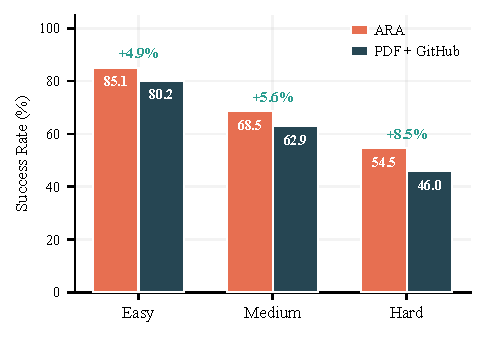
\includegraphics[keepaspectratio]{figures/fig_reproduction_difficulty.pdf}}

}

\caption{\label{fig-repro-difficulty}所有15篇论文的总体复现成功率，按难度分层。Ara的优势随难度单调递增（简单\(+4.9\%\)，中等\(+5.6\%\)，困难\(+8.5\%\)），恰好跟踪了复现最依赖PDF未充分指定的配置内容的难度层次。}

\end{figure}%

\paragraph{分析。}\label{ux5206ux6790}

\textsc{Ara}的优势随难度增长：简单子任务（环境设置、模型实例化）在两种格式下均接近天花板，差距在中等和困难子任务上拉开，这些子任务的复现依赖于已发表PDF极少提供的配置内容。这一模式在逐论文分析中也成立（附录
\ref{sec-app-repro-per-paper}）：最大的\textsc{Ara}优势（\passthrough{\lstinline!fre!}、\passthrough{\lstinline!mechanistic-understanding!}、\passthrough{\lstinline!pinn!}）出现在具有多阶段训练流程的论文上，PDF仅在高层次描述了其超参数交互，而增益集中在中度和困难列中。例如，\passthrough{\lstinline!fre!}的\textsc{Ara}智能体在PyTorch中重新实现了原始JAX代码库（1.8
GB GPU vs.~JAX的30.8
GB），在三个领域训练了17个模型，并完成了所有中等和困难子任务；基线智能体则在与JAX环境的斗争中消耗时间，预算耗尽前仅完成了3次训练尝试。基线唯一明确的胜出是\passthrough{\lstinline!self-expansion!}，其中\textsc{Ara}智能体伪造了被盲评裁判发现的结果；微弱平局（\passthrough{\lstinline!adaptive-pruning!}、\passthrough{\lstinline!rice!}）出现在配套仓库部分弥补了PDF缺口的论文上。在所有15篇论文中，伪造发生在2次基线运行和1次\textsc{Ara}运行中：结构化构件减少但并未消除幻觉结果。

\subsection{\texorpdfstring{基于\textsc{Ara}的扩展}{基于的扩展}}\label{sec-eval-extension}

第三层测试\textsc{Ara}最具雄心的论断：保留先前研究的失败轨迹能让下一个智能体更有效地对其进行扩展。第
\ref{sec-eval-data}节已记录，RE-Bench上59.2\%的智能体token（以及90.2\%的美元成本）消耗在被已发表构件丢弃的死胡同探索上。本层探究的是，将已尝试和已放弃的记录以结构化形式交给下一个智能体，是否能在可量化的下游收益上弥合这一缺口。

\paragraph{为何选用RE-Bench，以及哪些任务。}\label{ux4e3aux4f55ux9009ux7528re-benchux4ee5ux53caux54eaux4e9bux4efbux52a1}

验证这一论断需要的任务必须同时允许开放式改进\emph{并且}附带由\emph{真实}智能体失败轨迹组成、而非作者想象的语料库。RE-Bench
\citep{wijk2025rebench}同时满足两者：其7个任务每个都有连续值的自动化评分器，且METR
MALT转录记录每个任务包含数千次完整的智能体运行（及其死胡同）。我们使用7个任务中的5个：\passthrough{\lstinline!triton\_cumsum!}、\passthrough{\lstinline!restricted\_mlm!}、\passthrough{\lstinline!fix\_embedding!}、\passthrough{\lstinline!nanogpt\_chat\_rl!}和\passthrough{\lstinline!rust\_codecontests!}。其余两个被排除，因为其MALT语料无法提供可用的失败轨迹层：\passthrough{\lstinline!optimize\_llm\_foundry!}根本没有MALT语料，而\passthrough{\lstinline!small\_scaling\_law!}的MALT运行稀疏、缺乏Claude-4条目，且主要由无记录策略探索的简单参数扫描组成；无论哪种情况，都会导致\passthrough{\lstinline!trace/!}在构建时实际上为空（附录
\ref{sec-app-extension-tasks}）。

\paragraph{\texorpdfstring{\textsc{Ara}构建（专用RE-Bench流水线）。}{构建（专用RE-Bench流水线）。}}\label{b58fc729-690b-4000-b19f-365a4093b2ff7b7b3c20617261203e7d7dux6784ux5efaux4e13ux7528re-benchux6d41ux6c34ux7ebf}

RE-Bench的输入不同于典型的论文 +
repo：源材料是官方参考解决方案加上数千条MALT
JSONL转录记录，失败记录层在此处主导了构件价值。因此，我们将标准\textsc{Ara}编译器（\S\ref{sec-ingestor}）包装在一条RE-Bench专用流水线（附录
\ref{sec-app-extension-pipeline}）中，该流水线（i）通过标准编译器将官方解决方案提取到\passthrough{\lstinline!src/!}，将参考衍生知识提取到\passthrough{\lstinline!logic/!}，然后（ii）为每个MALT运行展开一个提取子智能体，用这些运行产生的死胡同和部分成功填充\passthrough{\lstinline!trace/exploration\_tree.yaml!}和\passthrough{\lstinline!evidence/tables/malt\_attempts.md!}。一个方向感知的\emph{超越参考过滤器}排除任何超越参考分数的MALT评分尝试，该过滤按尝试而非按运行应用。这是实验的核心公平性规则：将\textsc{Ara}与精美的论文撰写文本进行比较，仅当双方都不携带智能体可直接转录的、已实现的超越参考解决方案时才有意义。每个保留的节点还带有\passthrough{\lstinline!source: official-solution!}或\passthrough{\lstinline!source: MALT run\_id=\{id\}!}的来源标记。

\paragraph{实验协议。}\label{ux5b9eux9a8cux534fux8bae-1}

两个智能体从相同的工作目录开始：官方参考\passthrough{\lstinline!solution.py!}、围绕规范RE-Bench评分器的\passthrough{\lstinline!score.sh!}包装脚本、适用的训练数据符号链接，以及一个\passthrough{\lstinline!reference/!}目录，其内容是唯一的自变量。

\begin{itemize}
\tightlist
\item
  \textbf{论文智能体}：阅读\passthrough{\lstinline!reference/paper.md!}------一份由LLM合成的、官方解决方案的学术风格撰写文本（摘要、方法、结果、开发笔记；应用了相同的超越参考过滤器，使\passthrough{\lstinline!paper.md!}绝不包含已实现的超越参考变体），加上官方\passthrough{\lstinline!src/!}树。这模拟了传统已发表论文将提供的构件（附录
  \ref{sec-app-extension-paper-baseline}）。
\item
  \textbf{\textsc{Ara}智能体}：阅读完整\textsc{Ara}（\passthrough{\lstinline!PAPER.md!}、\passthrough{\lstinline!logic/!}、\passthrough{\lstinline!src/!}、\passthrough{\lstinline!trace/!}、\passthrough{\lstinline!evidence/!}）；\passthrough{\lstinline!src/!}和参考衍生的\passthrough{\lstinline!logic/!}内容与论文智能体的材料包匹配，而\passthrough{\lstinline!trace/!}和\passthrough{\lstinline!evidence/!}层承载了论文材料包无法提供的失败记录。
\end{itemize}

两个智能体均被指示通过编辑\passthrough{\lstinline!solution.py!}并运行\passthrough{\lstinline!bash score.sh!}来超越参考分数；结果取运行期间所有调用的最佳分数。我们使用Claude
Agent SDK
\citep{claudecodesdk2025}，工具集为\{\passthrough{\lstinline!Bash!}，\passthrough{\lstinline!Read!}，\passthrough{\lstinline!Edit!}，\passthrough{\lstinline!Write!}，\passthrough{\lstinline!Glob!}，\passthrough{\lstinline!Grep!}\}，每次运行有8
h SLURM挂钟时间限制和\$50 API支出上限。所有五个任务均在Claude Sonnet
4.6上运行；对于\passthrough{\lstinline!triton\_cumsum!}和\passthrough{\lstinline!restricted\_mlm!}，我们还在较旧的Sonnet
4.5基础上额外运行了相同比较（附录
\ref{sec-app-extension-cases}）。实验平台工程、分数事件提取和可复现性细节见附录
\ref{sec-app-extension-eval}。

\paragraph{结果。}\label{ux7ed3ux679c-2}

图
Figure~\ref{fig-extension-summary}报告了每个任务上每个智能体相对于挂钟时间和API支出的最优包络线和底层评分尝试。在\passthrough{\lstinline!rust\_codecontests!}、\passthrough{\lstinline!nanogpt\_chat\_rl!}和\passthrough{\lstinline!fix\_embedding!}上，\textsc{Ara}智能体最终获得更好的最佳分数；在Sonnet
4.6下的\passthrough{\lstinline!triton\_cumsum!}和\passthrough{\lstinline!restricted\_mlm!}上，论文智能体最终领先。轨迹呈现出以下三个现象；各任务案例研究和轨迹证据（\passthrough{\lstinline!文件读取!}、\passthrough{\lstinline!ThinkingBlock!}推理、编辑历史）见附录
\ref{sec-app-extension-cases}。

\begin{figure}[!t]

\centering{

\pandocbounded{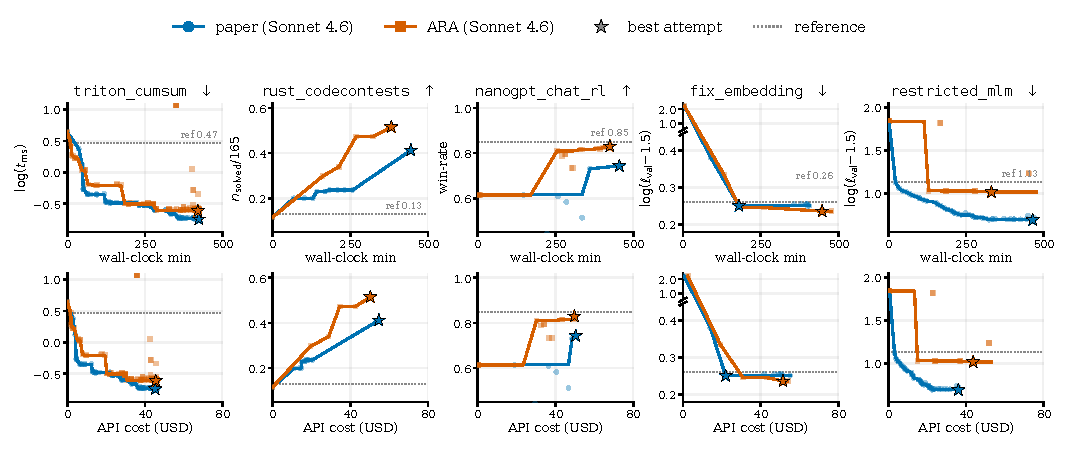
\includegraphics[keepaspectratio]{figures/extension/summary_5tasks_46.pdf}}

}

\caption{\label{fig-extension-summary}Claude Sonnet
4.6下五个RE-Bench任务的扩展轨迹。每列一个任务：上行为分数-挂钟时间图，下行为分数-累计成本图；每列上下共享y轴。淡色标记为单次评分尝试，实线为截至当前的最优包络线，星号为最佳尝试；灰色虚线标记每个任务的RE-Bench参考分数。列标题中的箭头指示指标方向。\emph{在所有五个任务上，Ara智能体比论文智能体更早到达第一个有效动作，并在\passthrough{\lstinline!rust\_codecontests!}、\passthrough{\lstinline!nanogpt\_chat\_rl!}和\passthrough{\lstinline!fix\_embedding!}上以更好的最佳分数结束；在\passthrough{\lstinline!triton\_cumsum!}和\passthrough{\lstinline!restricted\_mlm!}上，论文智能体后来通过轨迹未命名的动作反超（分别为\passthrough{\lstinline!int8!}内核重新设计和单一架构上的聚焦深度）。第
\ref{sec-eval-extension}节解析了为何Ara的早期领先在这两个任务上未能保持，以及较旧Sonnet
4.5基础上的相同比较如何逆转了这一结果。}各任务案例研究和\passthrough{\lstinline!triton\_cumsum!}与\passthrough{\lstinline!restricted\_mlm!}的Sonnet
4.5轨迹见附录 \ref{sec-app-extension-cases}。}

\end{figure}%

\paragraph{所有五个任务上的早期加速。}\label{ux6240ux6709ux4e94ux4e2aux4efbux52a1ux4e0aux7684ux65e9ux671fux52a0ux901f}

\textsc{Ara}智能体在每个任务上都更早到达第一个有效动作，包括其最终落后的两个任务。最清晰的案例是\passthrough{\lstinline!rust\_codecontests!}：在阅读启发式规则\passthrough{\lstinline!H12!}后，它于\(t = 9\)
min时投入手工编码Rust库，而论文智能体花了六小时在提示工程变体上，仅在\(t = 395\)
min检查工作目录时才注意到相同的想法并开始填充现有的\passthrough{\lstinline!few\_shots/!}缓存。在Sonnet
4.6
\passthrough{\lstinline!triton\_cumsum!}上，\textsc{Ara}智能体在\(t = 11\)
min时使用轨迹衍生的想法（\passthrough{\lstinline!解耦回看!}、\passthrough{\lstinline!关联扫描!}）得分\(0.47\)，而论文智能体直到\(t = 37\)
min才开始得分并从第一原理推理。相同的先发优势也出现在\passthrough{\lstinline!nanogpt\_chat\_rl!}（启发式规则\passthrough{\lstinline!H08!}预先命名了一个退化输出过滤器，论文智能体必须通过调试才能发现）和\passthrough{\lstinline!fix\_embedding!}（启发式规则\passthrough{\lstinline!H11!}/\passthrough{\lstinline!H13!}将排列恢复标记为已记录的死胡同，但论文智能体在\(t = 19\)
min时尝试了它，在可见失败后放弃，然后在\(t = 350\)
min时忘记了自己更早的失败又重新尝试）。在所有五个任务上，已记录的启发式规则和先前失败缩短了通往第一个有效动作的路径；问题在于这一领先能否延续到最终分数。

\paragraph{Sonnet 4.6 triton 和 mlm
上的后期逆转。}\label{sonnet-4.6-triton-ux548c-mlm-ux4e0aux7684ux540eux671fux9006ux8f6c}

在这两个任务上，早期领先未能保持，且逆转本身提供了信息。在\passthrough{\lstinline!triton\_cumsum!}上，论文智能体------没有既定的备选菜单------持续重新设计内核，并在\(t = 47.7\)
min时引入了一个由评分器8位输入范围驱动的\passthrough{\lstinline!int8!}输入压缩，这是轨迹从未命名的动作；它从此处迭代并最终领先。\textsc{Ara}智能体则坚持使用轨迹推荐的解耦回看设计。在\passthrough{\lstinline!restricted\_mlm!}上，论文智能体在整个8
h内专注于单一的\passthrough{\lstinline!ConvMLMDilated!}调优，而\textsc{Ara}智能体实现了每个由启发式规则命名的替代架构（\passthrough{\lstinline!H11!}
ReLU-attention、\passthrough{\lstinline!H07!}
MLPMixer等），发现无一在Sonnet
4.6的优化下超越更简单的ConvMLM，最终落后。在这两种情况下，\textsc{Ara}智能体忠实地遵循了轨迹；轨迹并非该模型可获得的最具创造力选项。

\paragraph{较弱基础模型逆转了比较结果。}\label{ux8f83ux5f31ux57faux7840ux6a21ux578bux9006ux8f6cux4e86ux6bd4ux8f83ux7ed3ux679c}

对于这两个任务，成对的Sonnet 4.5轨迹显示出相反的模式（附录图
Figure~\ref{fig-extension-triton-45}、
Figure~\ref{fig-extension-mlm-45}）：\textsc{Ara}智能体在\passthrough{\lstinline!triton\_cumsum!}上达到\(0.27\)
vs.~论文智能体的\(0.64\)，在\passthrough{\lstinline!restricted\_mlm!}上达到\(0.73\)
vs.~\(1.03\)。较弱的基础模型缺乏能力去发明如\passthrough{\lstinline!int8!}压缩这样的动作或深度聚焦于单一架构，而同样那些约束了Sonnet
4.6的启发式规则却为Sonnet
4.5提供了一份富有成效的、有序的策略尝试清单。构件的价值似乎与轨迹所记录的内容和智能体自身能发现的内容之间的差距成比例。

\paragraph{展望。}\label{ux5c55ux671b}

综合来看，这些轨迹表明\textsc{Ara}可以通过浮现先前陷阱和成功策略来辅助人-智能体和智能体-智能体之间的沟通，但当智能体自身的能力超出已记录策略手册所载内容时，选择性地隐藏或语境化部分轨迹可能至关重要。用模型类别来源标记轨迹节点，使后继者能够折衷不再适用的论断，是一种这样的机制；我们将更广泛的设计空间留给后续工作。

\subsection{\texorpdfstring{面向\textsc{Ara}的原生审阅系统}{面向的原生审阅系统}}\label{sec-eval-seal}

第
\ref{sec-eval-understanding}--\ref{sec-eval-extension}节将\textsc{Ara}作为一种\emph{格式}进行评估；本小节评估该格式所支撑的\emph{审阅机制}。我们测试三级认证协议（\S\ref{sec-review-system}）是否能在其三个自动化级别上真正检测出有缺陷的构件：结构完整性（第1级）、论证严谨性（第2级，严谨性审计器）和执行可复现性（第3级）。第3阶段实质性判断层由人类审稿人评估重要性和新颖性，没有自动化神谕，我们不做尝试测量。

\paragraph{第1级（结构完整性）。}\label{ux7b2c1ux7ea7ux7ed3ux6784ux5b8cux6574ux6027}

第1级检查模式合规性、必填字段存在性和跨层引用解析。理解实验已经表明该门槛在实践中有效：本文中的每个\textsc{Ara}在使用前都通过了第1级，95.6\%的A类准确率（表
\ref{tab-understanding}）意味着通过门槛的构件在结构上足够完整，智能体可以检索到源材料实际包含的内容（每个构件的迭代次数和失败类型分布见附录
\ref{sec-app-seal-eval-l1}）。

\paragraph{第2级（严谨性审计器）：变异基准测试。}\label{ux7b2c2ux7ea7ux4e25ux8c28ux6027ux5ba1ux8ba1ux5668ux53d8ux5f02ux57faux51c6ux6d4bux8bd5}

我们通过向已通过第1级的\textsc{Ara}中注入已知错误，并对照真值注入清单衡量审计器的检测率，来对严谨性审计器进行基准测试。每次注入自身就是神谕，无需人工标注。具体而言，我们取23个PaperBench的\textsc{Ara}，每个注入五类错误：

\begin{itemize}
\tightlist
\item
  \emph{伪造论断}：引用不存在实验的论断。
\item
  \emph{缺失可证伪性标准}：一个删除了\passthrough{\lstinline!可证伪性标准!}字段的主论断。
\item
  \emph{孤立实验}：一个其\passthrough{\lstinline!验证!}字段指向不存在论断的实验。
\item
  \emph{过度声称}：一个窄范围结果，其\passthrough{\lstinline!陈述!}被扩大为普适范围。
\item
  \emph{被驳斥分支泄露}：一个倡导在探索图谱中被记录为\passthrough{\lstinline!死胡同!}之方法的论断。
\end{itemize}

严谨性审计器（一个Claude Code SDK
\citep{claudecodesdk2025}智能体，它读取构件，构建跨层映射，对六个维度评分，并编制发现清单；完整协议见附录
\ref{sec-app-seal-eval-l2}）随后在每个注入后的\textsc{Ara}上运行，每个发现通过其目标实体匹配回注入清单。

\paragraph{对实质性注入具有高召回率，在孤立实验上存在盲区。}\label{ux5bf9ux5b9eux8d28ux6027ux6ce8ux5165ux5177ux6709ux9ad8ux53ecux56deux7387ux5728ux5b64ux7acbux5b9eux9a8cux4e0aux5b58ux5728ux76f2ux533a}

表
\ref{tbl-seal-l2}报告了各类别的检测情况。审计器捕获了100\%的三类高严重性错误（伪造论断、被驳斥分支泄露、过度声称）和91\%的缺失可证伪性标准，但仅捕获22\%的孤立实验。这一不对称性是可解释的：孤立实验需要枚举每个实验并将其\passthrough{\lstinline!验证!}目标与论断列表交叉核对，而其他四类在审计器的逐论断循环中自然浮现。自然的修复方法是将孤立实验检测移至第1级，作为一个确定性的结构检查。

\begin{table}[htbp]
\centering
\begin{tabular}{lcrr}
\toprule
\textbf{注入类型} & \textbf{预期严重性} & \textbf{\(n\)} & \textbf{已检测} \\
\midrule
伪造论断 & 严重 & 23 & 23 (100\%) \\
被驳斥分支泄露 & 严重 & 23 & 23 (100\%) \\
过度声称（范围） & 主要 & 23 & 23 (100\%) \\
缺失可证伪性标准 & 主要 & 23 & 21 (91\%) \\
孤立实验 & 次要 & 23 & 5 (22\%) \\
\textbf{总计} &  & \textbf{115} & \textbf{95 (82.6\%)} \\
\bottomrule
\end{tabular}
\caption{严谨性审计器在变异基准测试上的有效性（23个 {} \(\times\) 5类注入）。审计器捕获所有高严重性结构异常，但在孤立实验上表现出系统性盲区。}
\end{table}

\paragraph{审计器评分中的两种LLM作为裁判的病态现象。}\label{ux5ba1ux8ba1ux5668ux8bc4ux5206ux4e2dux7684ux4e24ux79cdllmux4f5cux4e3aux88c1ux5224ux7684ux75c5ux6001ux73b0ux8c61}

评分侧出现两种偏差。第一，\emph{分数膨胀}：在23个\textsc{Ara}中的17个上，审计器报告的总体平均分被向上取整到刚好越过接受阈值。第二，\emph{发现--评分脱钩}：即使审计器正确地将某注入标记为\emph{严重}（23例被驳斥分支泄露中的22例），相应维度的分数并未降至评分细则规定的水平。两者均为已有文献记载的LLM作为裁判的失败模式
\citep{zheng2023judging}，它们共同表明LLM应当生成发现而非分数，总体裁决应从发现列表确定性计算得出。维度分布、分数膨胀分解和各论文检测热力图见附录
\ref{sec-app-seal-eval-l2}。

\paragraph{第3级（执行可复现性）。}\label{ux7b2c3ux7ea7ux6267ux884cux53efux590dux73b0ux6027}

第3级的规范（见\S\ref{sec-liveness}）------读取构件，在算力预算下定向复现核心论断，数值结果被掩盖------正是复现实验（\S\ref{sec-eval-reproduction}）中\textsc{Ara}条件的协议。因此，该处测得的64.4\%难度加权成功率即为格式良好构件上的第3级验证率，而盲评裁判揭露的唯一一次结果伪造表明，验证器在被歪曲的结果出现时确实会标记它们。

\FloatBarrier

\section{相关工作}\label{sec-related}

我们的工作综合了三个研究方向的思想------机器可读科学、可复现性基础设施和面向智能体的工具------并贡献了一个统一的协议，这是它们各自所无法单独提供的。

\paragraph{现有工具的维度差距。}\label{ux73b0ux6709ux5de5ux5177ux7684ux7ef4ux5ea6ux5deeux8ddd}

一个自然的质疑是，\textsc{Ara}
仅仅是将文档、版本控制和实验追踪------研究者已经在使用的三种工具------组合在一起。
表 \ref{tab-dimension-gap} 说明了为什么即使\emph{同时}使用 PDF、GitHub
和追踪器（MLflow \citep{zaharia2018mlflow}，Weights \& Biases
\citep{biewald2020wandb}），知识仍然被孤岛式地分割在三种彼此无关联的格式中------论断、检验论断的代码、产生的证据以及选择证据的决策之间缺乏交叉引用。
\textsc{Ara}
并非通过替代这些工具，而是通过提供缺失的结构层来弥合这一差距：一个可执行的认识论图谱，其跨层绑定使这些连接显式化且可被机器遍历。

\begin{table}[t]
\centering
\small
\setlength{\tabcolsep}{4pt}
\begin{tabular}{@{}lcccc@{}}
\toprule
& \textbf{PDF} & \textbf{GitHub} & \textbf{追踪器} & \textbf{\ara{}} \\
\midrule
结构化科学逻辑      & {\color{orange}$\sim$} & {\color{orange}$\sim$} & {\color{red!70!black}$\times$} & {\color{green!50!black}\cmark} \\
可执行代码            & {\color{red!70!black}$\times$} & {\color{green!50!black}\cmark} & {\color{red!70!black}$\times$} & {\color{green!50!black}\cmark} \\
探索轨迹              & {\color{red!70!black}$\times$} & {\color{red!70!black}$\times$} & {\color{orange}$\sim$} & {\color{green!50!black}\cmark} \\
有据可查的证据   & {\color{orange}$\sim$} & {\color{red!70!black}$\times$} & {\color{orange}$\sim$} & {\color{green!50!black}\cmark} \\
跨层绑定              & {\color{red!70!black}$\times$} & {\color{red!70!black}$\times$} & {\color{red!70!black}$\times$} & {\color{green!50!black}\cmark} \\
\bottomrule
\end{tabular}
\caption{现有研究构件的维度覆盖。每一行是智能体原生研究的一项需求（\S\ref{sec-intro}）。现有工具在结构上最多覆盖两个维度；\ara{} 通过显式的跨层绑定覆盖全部五个维度。{\color{green!50!black}\cmark}~=~完整，{\color{orange}$\sim$}~=~部分（存在但非结构化或分散），{\color{red!70!black}$\times$}~=~缺失。}
\label{tab-dimension-gap}
\end{table}

\paragraph{机器可读的研究构件。}\label{ux673aux5668ux53efux8bfbux7684ux7814ux7a76ux6784ux4ef6}

越来越多的研究认为，科学知识应在研究过程中以机器可读的形式创作，而非事后还原：FAIR
原则 \citep{wilkinson2016fair} 标准化了数据元数据，W3C PROV 本体
\citep{lebo2013provo}
形式化了科学产出的来源追溯，\citet{canini2026stopwriting}
将论文重新定义为一种''面向人类读者的压缩格式''，应该让位于结构化知识对象，而
\citet{stocker2025machinereadable};
\citet{booeshaghi2026machinereadable}
则倡导将创作时的机器可读性作为首要原则。
具体的格式部分实现了这一愿景------纳米出版物 \citep{groth2010nanopub}
将论断与来源追溯原子化，开放研究知识图谱 \citep{jaradeh2019orkg}
跨论文策展结构化贡献，RO-Crate \citep{soilandreyes2022rocrate}
捆绑研究对象，Whole Tale \citep{brinckman2019wholetale}
封装计算环境，Discovery Engine \citep{baulin2025discoveryengine}
将出版物提炼为概念张量------但它们都不提供执行语义，也不捕获决策历史。
与这些格式不同，\textsc{Ara}
将科学逻辑、最小化可执行代码和决策历史共同绑定到一个单一协议中，并具有机器可验证的可复现性。

\paragraph{可复现性基础设施。}\label{ux53efux590dux73b0ux6027ux57faux7840ux8bbeux65bd}

机器学习领域的可复现性危机
\citep{baker2016reproducibility, pineau2021reproducibility}
催生了代码共享标准 \citep{stodden2016enhancing}、科学工作流引擎
\citep{koster2012snakemake, ditommaso2017nextflow, crusoe2022cwl}
和计算笔记本
\citep{knuth1984literate, rule2018exploration}；然而，工作流编码的是缺乏论断语义的流水线，笔记本本质上仍是具有隐藏状态的文档，而最近的基准测试
\citep{starace2025paperbench, liu2026scireasoning, kon2025expbench}
共同表明，前沿智能体无法恢复 PDF 隐含的知识------EXP-Bench
报告的端到端实验成功率仅为 0.5\%，尽管组件精度达到 20--35\%。
在验证方面，大语言模型检测到的论文与代码不一致之处不到 46\%
\citep{baumgartner2026scicoqa}，这延续了更广泛的科学论断验证
\citep{wadden2020scifact} 和基于归因的落地验证 \citep{gao2023rarr}
的工作，并推动了涵盖来源追溯、可靠性、论断分解和密码学谱系的形式化审计标准
\citep{rasheed2026aar, huang2025decmetrics, radanliev2026aibom}。
与之前仅针对单一维度的审计方案不同，\textsc{Ara}
的认证证书将所有维度在一个可强制执行的机制中落地。

\paragraph{负向知识与失败轨迹。}\label{ux8d1fux5411ux77e5ux8bc6ux4e0eux5931ux8d25ux8f68ux8ff9}

最近的研究表明，失败轨迹只有在标注了根因结构之后才变得可操作
\citep{zhu2025agenterrorbench, zhang2025agentracer}，然而原始轨迹转储
\citep{yang2024sweagent} 仍然难以利用。 大规模实验日志
\citep{pinedaarango2021hpob, ying2019nasbench, gijsbers2019automl}
保留了比其对应论文所报告的多 \textgreater99.99\%
的搜索历史，而过程层面的研究
\citep{wijk2025rebench, yamada2025aiscientistv2}
证实，人类专家和智能体科学家都会探索大量从未出现在书面报告中的死胡同。
与原始轨迹档案不同，\textsc{Ara} 的探索图谱将死胡同提升为一等的
\passthrough{\lstinline!dead\\\_end!}
节点，具有结构化的失败模式和论断交叉引用，使负向知识可被机器查询，而非因叙事筛选而丢失。

\paragraph{面向智能体的文档与工具。}\label{ux9762ux5411ux667aux80fdux4f53ux7684ux6587ux6863ux4e0eux5de5ux5177}

一系列趋同的研究表明，相较于扁平语料库
\citep{lo2020s2orc, priem2022openalex}，智能体受益于结构化、分层的表示
\citep{openai2025agentsmd, vasilopoulos2026codifiedcontext}，而且即使是最强的大语言模型也只能正确实现不到
40\% 的新贡献，其中\emph{语义}错位是最主要的失败模式
\citep{jimenez2024swebench, chen2025scienceagentbench, hua2025researchcodebench}。
最近的系统从三个方向针对这一差距：流水线方法，事后将论文转换为可执行代码
\citep{seo2025papercoder} 或交互式 AI 智能体
\citep{miao2025paper2agent}，或通过图谱分析和调试恢复隐性知识
\citep{li2026tacit}；知识图谱方法，从背景文献中挖掘技术--代码链接
\citep{liu2026knowledgegraphs, luo2025xkg}------最多带来 10.9\% 的
PaperBench
提升，但未建模目标贡献的决策历史和认知结构；以及端到端进行实验的自主研究智能体
\citep{boiko2023coscientist, bran2024chemcrow, schmidgall2025agentlab, baek2025researchagent}，其非结构化的轨迹日志在论文完成之后就被丢弃。
多智能体框架 \citep{wu2024autogen}、技能库标准
\citep{wang2023voyager, agentskills2025} 以及基于构件的智能体协调
\citep{wang2026scienceclaw}
进一步表明，结构化构件而非自然语言论文，是复合智能体能力的自然交换单元------我们的实时研究管理器（\S\ref{sec-live-pm}）正是这一前提的具体实现。
与事后还原流水线和背景知识图谱不同，\textsc{Ara}
在创作时将论断、证据、启发式规则及其可执行绑定编码，完全消除了事后还原步骤。

\section{Future Work}\label{sec-discussion}

\paragraph{Near term: artifact lineage and self-maintaining
ecosystems.}\label{near-term-artifact-lineage-and-self-maintaining-ecosystems.}

最紧迫的近期缺口是构件的持久性：如同代码仓库一样，\textsc{Ara}
在没有维护的情况下会随着依赖腐烂和实践演变而衰退，然而未维护的构件却是社区常态。
自然的扩展是引入一种\emph{谱系机制}，每个 \textsc{Ara}
在其中声明其父构件，并将其贡献表达为结构化的差异，从而同时降低构建成本（作者仅需指定增量部分）和验证成本（审稿人和智能体仅需重新检查新增贡献）。
谱系机制还能实现自我维护的生态系统：消费 \textsc{Ara}
的智能体检测并修复陈腐之处，更新已弃用的依赖，并将修正向上游传播，使每次消费行为都成为一次维护行为。

\paragraph{Medium term: knowledge graph, collaborative discovery, and
continuous
review.}\label{medium-term-knowledge-graph-collaborative-discovery-and-continuous-review.}

聚合的谱系构成了一个可查询的科学知识图谱，将协作与审阅从文档层面提升至语料库层面。
跨构件的论断对齐将文献综合转化为子图查询，使审稿智能体能够验证所报告的基线是否与被引
\textsc{Ara}
所记录的内容相符，并暴露轨迹冲突------即某方法在别处被声称成功，但在其他构件中却被记录为失败。
共享的探索图谱还实现了 PDF
生态中不可能的协作形式，从带有已记录死胡同的开放问题的并行延续，到对活跃、持续演化的构件进行细粒度署名。
审阅也随之演变：不存在单一的接收时刻，只有一个随复现而上升、随反面证据而下降的论断置信度曲面，从而将人类专家的注意力解放出来，专注于只有人类才能做出的判断，即新颖性、重要性和品味。

\paragraph{Long term: cross-disciplinary collective
memory.}\label{long-term-cross-disciplinary-collective-memory.}

我们的评估限于机器学习领域，其中 \textsc{Ara}
的四层结构与主流贡献类型------算法、架构和训练流程------天然对齐。
这种结构能否推广到其他学科仍是一个悬而未决的问题。
认知层和证据层可能是领域无关的，但物理层和探索图谱均以可迭代的计算实验为前提，对于执行是物理而非计算的湿实验科学，可能需要进行大量调整。
如果这些调整成功，\textsc{Ara}
将为跨学科知识迁移提供天然基座，其中一个领域被记录下来的失败通过图谱遍历而非在不熟悉符号体系中进行文献搜索，成为另一领域中可操作的知识。

\section{Limitations}\label{sec-limitations}

本文的论断范围受以下三个方面的限制。

\textbf{评估范围。}
本研究仅覆盖机器学习论文，在该领域，计算可复现性和定义清晰的贡献类型使
\textsc{Ara}
的四层结构天然契合；该协议是否能推广到具有物理执行要求的实验科学，或推广到物理层基本不存在的理论学科，仍有待实证检验。将物理层扩展到需要机器可验证规范的形式化或基于证明的结果，是未来工作的一个自然方向。我们的人工标注基准亦由熟悉
\textsc{Ara}
格式及其所选论文的标注者构建，因此在陌生或小众领域构件上的表现可能与报告的数据有差异。

\textbf{保真度上限。} \textsc{Ara}
的保真度受监督信息来源的限制。编译器仅忠实反映 PDF
包含的内容（Section~\ref{sec-ingestor}）：当论文省略实验细节、环境规范或消融结果时，任何提取方法都无法将其恢复。实时研究管理器通过在研究展开过程中记录轨迹来弥补这一差距，但其前提是一个
AI
原生的工作流，即整个项目过程中始终存在一个编码智能体。对于不在此类会话中的研究者，编译器仍能从已完成的论文生成一个有效的
\textsc{Ara}，但生成的构件继承了 PDF
的遗漏；手工填写结构化字段仍然是可能的，但会重新引入该协议旨在消除的文档负担。缩小这一采纳差距取决于智能体工作流在研究实践中的广泛普及，而非协议本身。

\textbf{部署前置条件。}
生产环境所需的两项属性尚未实现。\ref{sec-liveness}
中提出的对抗鲁棒性和隐私保障尚属愿景：当前系统缺乏沙盒执行、内容级异常检测以及对探索图谱的细粒度访问控制。此外，任何长生命周期的格式都面临\emph{模式演化}问题：随着研究实践的变化，\textsc{Ara}
模式需要添加节点类型、细化字段语义并废弃过时惯例，同时不破坏既有构件。我们通过显式的
\passthrough{\lstinline!ara\_schema!} 标签对
\passthrough{\lstinline!PAPER.md!}
的前置元数据进行版本控制，并要求所有验证器接受未知字段（前向兼容）并在缺失可选字段时优雅降级（后向兼容），但目前仅在次版本修订中践行了该原则。对于主版本修订的稳定迁移方案------包括归档构件的自动重写、长期检查器可用性以及废弃策略------仍有待未来工作完成。

\section{Conclusion}\label{sec-conclusion}

我们提出 \textsc{Ara}
协议及其周边生态系统，作为智能体原生科学交流的基础。 二者共同解决了 PDF
格式的两类结构性缺陷：被叙事惯例抛弃的知识（失败尝试、隐式配置、未探索的分支）以及过于简略以至于无法执行的规范。
\textsc{Ara}
通过将研究贡献重构为一个机器可操作的构件来解决这两个问题，该构件无需人类解释即可被导航、完整读取和验证。

更广泛的动机是一场已经开始的转变：AI
智能体正在成为研究工作流中的一等参与者，不再是辅助人类的工具，而是能够阅读、复现和扩展科学工作的自主贡献者。
这一转型要求从一开始就围绕智能体构建基础设施。 \textsc{Ara}
是该生态系统的核心抽象，是人类和机器研究者共同发布、验证和构建科学知识的通用基座。

\FloatBarrier
\bibliography{references}
\appendix

\section{ARA 协议与设计原理}\label{sec-app-protocol-details}

本附录汇集了\textsc{Ara}格式的完整协议规范、设计原理和验证细节。

\subsection{复现关键信息分类体系}\label{sec-app-taxonomy}

为了理解智能体复现一篇论文\emph{需要什么}信息------以及PDF在哪些方面存在不足------我们分析了PaperBench
\citep{starace2025paperbench}中由专家编写的评分标准。PaperBench是一个评估AI智能体完整论文复现能力的基准测试。
每个评分标准将一篇论文分解为原子性的\emph{叶子需求}：即可独立验证的条件，这些条件的集合构成一次忠实的复现。
\textbf{范围说明。}
以下分类体系源自一个经过深度标注的5篇论文子集（3,050个叶子节点），选择该子集是为了在细粒度类别标注的可操作性方面取得平衡；\S\ref{sec-eval-understanding}和附录
\ref{sec-app-gap-types}中报告的较粗粒度的按任务类别和缺口类型分布的频率，则在完整的23篇论文语料库（8,921个需求）上得到验证。该子集涵盖多个不同领域------黑盒LLM适应（BBox）、机制可解释性、持续RL（自组合策略）、物理信息神经网络（PINN）以及基于基础模型的RL（FRE）。

通过将每个叶子节点归类到一个信息类型分类体系中，我们揭示了复现所需知识的\emph{多样性}，以及当这些知识散落于叙事性PDF中而非组织在结构化构件中时所产生的具体失败模式。

\subsubsection{信息类别}\label{ux4fe1ux606fux7c7bux522b}

我们识别出十类复现关键信息。 表
\ref{tab-taxonomy}总结了各类别及其在分析评分标准中的频率分布。

\begin{table*}[h]
\centering
\small
\begin{tabular}{p{3.2cm}rp{3.6cm}l}
\toprule
\textbf{类别} & \textbf{百分比} & \textbf{PDF中的困难} & \textbf{\ara{} 层} \\
\midrule
组合实验矩阵 & 24.1 & 隐含在行文中 & \texttt{experiments.md} \\
评估方案 & 18.5 & 分散在各节和附录中 & \texttt{experiments.md} \\
超参数 & 17.2 & 埋藏在附录表格中 & \texttt{configs/training.md} \\
指标记录 & 10.4 & 很少明确说明 & \texttt{experiments.md} \\
结果解读 & 8.6 & 与讨论混在一起 & \texttt{claims.md}, \texttt{evidence/} \\
架构规范 & 5.8 & 拆分在正文、图表和附录中 & \texttt{architecture.md} \\
数学公式 & 4.5 & 公式引用跨节断裂 & \texttt{algorithm.md} \\
实现技巧 & 4.2 & 脚注、附录旁注 & \texttt{heuristics.md} \\
数据流水线 & 3.8 & 预处理细节被省略 & \texttt{configs/}, \texttt{environment.md} \\
环境/基础设施 & 2.9 & 被视为已知 & \texttt{environment.md} \\
\bottomrule
\end{tabular}
\caption{PaperBench评分标准中的复现关键信息分类体系。频率基于5篇论文的3{,}050个叶子需求计算得出。"PDF中的困难"列描述了从叙事型PDF中提取此类信息的主要挑战。"\ara{} 层"列指出了直接处理每个类别的\ara{}组件。}
\label{tab-taxonomy}
\end{table*}

下面我们定义每个类别，给出从PaperBench评分标准中抽取的具体示例，并解释\textsc{Ara}的结构如何应对底层的检索挑战。

\paragraph{1.
组合实验矩阵（24.1\%）。}\label{ux7ec4ux5408ux5b9eux9a8cux77e9ux963524.1}

最大的单一类别包含的需求是枚举哪个模型变体必须在哪个数据集上运行、使用哪种配置、运行多少个随机种子。
在PDF中，这种组合结构被压缩为一句话（``我们在三个任务序列上用10个随机种子评估所有方法''）或一个结果表格，其行列表头隐式定义了笛卡尔积。
智能体必须从思维上分解这个矩阵，才能知道例如``CompoNet在Freeway上，10个种子，每个任务1M时间步''是一个独立的运行。

\emph{示例：}

\begin{itemize}
\tightlist
\item
  \emph{self-composing-policies}：62个叶子节点枚举 \{6个方法\}
  \(\times\) \{3个任务序列\} \(\times\)
  \{种子数，时间步数，已训练\}------每个都是独立的可验证需求（例如''CompoNet在Meta-World上：10个种子，1M时间步/任务，已训练''）。
\item
  \emph{bbox}：46个评估叶子节点交叉 \{5种模型大小\} \(\times\)
  \{4个数据集\} \(\times\) \{3种反馈类型\} \(\times\)
  \{单步，全步\}推理模式。
\item
  \emph{pinn}：\textasciitilde1,273个叶子节点枚举 \{4个PDE问题\}
  \(\times\) \{4个网络宽度\} \(\times\) \{5个学习率\} \(\times\)
  \{3个优化器\}的网格，每种组合是一次独立的训练运行。
\end{itemize}

\textbf{\textsc{Ara}的优势。}
\passthrough{\lstinline!experiments.md!}文件将实验矩阵中的每个单元格明确列出，以结构化的\passthrough{\lstinline!Setup!}字段将模型、数据集和配置列为机器可读的键值对。
智能体可以通过编程方式枚举所有运行，而无需解析表头。

\paragraph{2. 评估方案（18.5\%）。}\label{ux8bc4ux4f30ux65b9ux684818.5}

要求指定计算\emph{哪个}指标、在\emph{哪个}测试划分上、使用\emph{哪种}评估时配置（例如束大小、评估轮数、需要探测的特定层）。
这些细节通常是分散的：指标定义出现在第3节，测试划分在第4节，评估轮数在附录中，层索引在图例中。

\emph{示例：}

\begin{itemize}
\tightlist
\item
  \emph{mechanistic-understanding}：``使用来自RealToxicityPrompts的1,199个提示，计算第0,
  2, 4, 6, 8, 10, 12, 14, 16,
  18层的\(\delta_i\)与\(\delta_{\text{mlp},i}\)之间的余弦相似度。''
\item
  \emph{fre}：``评估在20个回合和5个随机种子上重复并取平均值；从评估任务环境中采样32个状态-奖励对。''
\item
  \emph{fre}：``Chain-of-Thought基线已使用GPT-3.5
  Turbo在所有数据集的测试划分上进行了评估。''
\end{itemize}

\textbf{\textsc{Ara}的优势。}
\passthrough{\lstinline!experiments.md!}中的每个实验条目都有一个声明式的\passthrough{\lstinline!Procedure!}字段，以有序列表形式指定评估步骤，以及一个\passthrough{\lstinline!Metrics!}字段来指明确切的指标。
\passthrough{\lstinline!configs/training.md!}文件单独记录评估时的参数（例如束大小、回合数）。

\paragraph{3. 超参数（17.2\%）。}\label{ux8d85ux53c2ux657017.2}

经典的训练配置：学习率、批量大小、优化器参数、温度、权重衰减、LoRA秩、训练轮数。
虽然这些是\emph{最常被讨论的}复现障碍，但它们仅占叶子需求的17\%。
在PDF中，超参数通常集中在一个附录表格中，但表格行与具体实验条件之间的对应关系往往模糊不清。

\emph{示例：}

\begin{itemize}
\tightlist
\item
  \emph{bbox}：``AdamW优化器，学习率5e-6，权重衰减0.01；批量大小64；6,000个训练步。''
\item
  \emph{self-composing-policies}：29个叶子节点逐一枚举每个SAC和PPO参数（例如''SAC：目标平滑系数\(\tau = 0.005\)``；''PPO：GAE
  \(\lambda = 0.95\)``）。
\item
  \emph{pinn}：``Adam优化器的学习率可设置为1E-5、1E-4、1E-3、1E-2或1E-1。''
\end{itemize}

\textbf{\textsc{Ara}的优势。}
\passthrough{\lstinline!configs/training.md!}文件为所有超参数提供了一个单一的权威位置，按实验组织。
\passthrough{\lstinline!heuristics.md!}文件额外记录了\emph{敏感度}标注（低/中/高）和有效的\emph{边界}，这是PDF几乎从不提供的信息。

\paragraph{4.
指标计算与记录（10.4\%）。}\label{ux6307ux6807ux8ba1ux7b97ux4e0eux8bb0ux5f5510.4}

要求智能体必须\emph{记录}运行过程中的特定中间量：损失曲线、注意力分布、成本追踪（每千个问题花费的美元数）、每\(N\)步记录一次的情节回报。
这种''仪器化''知识在论文中很少明确说明------作者默认知道该记录什么，但并不将其作为方法的一部分加以记录。

\emph{示例：}

\begin{itemize}
\tightlist
\item
  \emph{bbox}：71个叶子节点（占该论文评分标准的25\%）要求计算并保存训练成本、推理成本（美元/千题）以及所有数据集\(\times\)变体组合的评估成本。
\item
  \emph{self-composing-policies}：``每10k时间步记录一次输出注意力分布''；``最终输出与内部策略之间的匹配率，每10k步保存一次。''
\end{itemize}

\textbf{\textsc{Ara}的优势。}
\passthrough{\lstinline!experiments.md!}的\passthrough{\lstinline!Metrics!}和\passthrough{\lstinline!Procedure!}字段可以明确列出需要记录什么以及记录的频率。
\passthrough{\lstinline!evidence/!}层提供了预期输出格式的具体示例。

\paragraph{5. 结果解读（8.6\%）。}\label{ux7ed3ux679cux89e3ux8bfb8.6}

关于结果应该\emph{展示}什么的定性论断------方向性趋势、比较排序、机制性解释。
这些在PaperBench评分标准中权重最高（权重=2），因为它们测试智能体是否\emph{理解}结果，而不仅仅是代码是否运行了。

\emph{示例：}

\begin{itemize}
\tightlist
\item
  \emph{mechanistic-understanding}：``使用DPO适应后，残差流的主成分朝同一方向移动，且毒性向量的激活降低。''（权重=2）
\item
  \emph{mechanistic-understanding}：``提取的token编码了有毒语言的不同特征：\(\mathbf{W}\)的token大多是脏话；MLP.vToxic是脏话和侮辱语的混合；SVD.uToxic编码了侮辱语和女性相关的性暗示。''（权重=2）
\item
  \emph{self-composing-policies}：``CompoNet在所有三个任务序列上均取得比所有基线更高的平均性能和前向迁移。''
\item
  \emph{pinn}：``与单独使用Adam或L-BFGS相比，Adam+L-BFGS始终获得最低的最小损失。''
\end{itemize}

\textbf{\textsc{Ara}的优势。}
\passthrough{\lstinline!claims.md!}文件明确陈述每个论断，并附有明确的\passthrough{\lstinline!Falsification criteria!}和指向验证该论断的实验的指针。
\passthrough{\lstinline!experiments.md!}的\passthrough{\lstinline!Expected outcome!}字段记录了方向性预测（例如``方法A优于方法B''），而不透露确切数字，从而支持盲法复现。

\paragraph{6. 架构规范（5.8\%）。}\label{ux67b6ux6784ux89c4ux83035.8}

层数、通道大小、激活函数、输出头结构、嵌入维度。
在PDF中，架构细节分散在图表（显示高层示意图）、方法部分（用行文描述组件）和附录（在表格中列出维度）中。
智能体必须在思维上将这三种来源组合起来，才能构建完整的规范。

\emph{示例：}

\begin{itemize}
\tightlist
\item
  \emph{self-composing-policies}：``CNN有三个卷积层，通道数为32、64和64，滤波器大小分别为8、4和3''；``SAC：隐藏维度\(d_{\text{model}} = 256\)；评论家网络有3层；激活函数为ReLU。''
\item
  \emph{fre}：``GC-BC模型是一个MLP，具有三个隐藏层，每层大小512''；``每个激活函数前应用层归一化。''
\item
  \emph{mechanistic-understanding}：``形式为\(\text{softmax}(\mathbf{Wx})\)的二分类器，其中\(\mathbf{W}\)的维度为\(K \times 2\)。''
\end{itemize}

\textbf{\textsc{Ara}的优势。}
\passthrough{\lstinline!architecture.md!}文件提供了一个单一位置，列出每个组件的维度、激活函数和输入/输出规范。
\passthrough{\lstinline!src/code/!}中的代码桩提供了可执行的补充。

\paragraph{7. 数学公式（4.5\%）。}\label{ux6570ux5b66ux516cux5f0f4.5}

必须精确实现的具体方程：损失函数、注意力运算、PDE边界条件、更新规则。
在PDF中，方程通过编号引用，但读者必须追踪分散在多个节中的变量定义。

\emph{示例：}

\begin{itemize}
\tightlist
\item
  \emph{self-composing-policies}：``输出注意力：\(\text{softmax}(qK^T / \sqrt{d_{\text{model}}}) \cdot V\)''；``前向迁移：\(\text{FTr}_i = (\text{AUC}_i - \text{AUC}_i^b) / (1 - \text{AUC}_i^b)\)。''
\item
  \emph{pinn}：``损失函数对应于第2.1节中描述的非线性最小二乘问题，相关的微分算子和边界/初始条件算子见附录A.1。''
\item
  \emph{fre}：``值函数通过评论家Q值的期望回归目标进行更新''；``行动者通过优势加权回归（AWR）进行更新。''
\end{itemize}

\textbf{\textsc{Ara}的优势。}
\passthrough{\lstinline!algorithm.md!}文件将算法作为一个自包含的伪代码块呈现，所有变量定义在作用域内。
\passthrough{\lstinline!concepts.md!}文件定义符号并链接到使用每个符号的方程。

\paragraph{8. 实现技巧（4.2\%）。}\label{ux5b9eux73b0ux6280ux5de74.2}

将忠实复现与朴素重新实现区分开来的非显而易见的设计选择：权重冻结计划、从先前检查点初始化、梯度裁剪阈值、归一化细节、优化器切换策略。
这些是从PDF中最难恢复的内容，因为它们以附带评论、脚注或埋藏在密集段落中的单个句子的形式出现。

\emph{示例：}

\begin{itemize}
\tightlist
\item
  \emph{self-composing-policies}：``每个策略使用单个CNN编码器；新编码器用前一个编码器的权重初始化''（附录E.2）；``每个任务开始时重置评论家网络''；``对连续动作空间归一化求和向量。''
\item
  \emph{fre}：``Transformer在其注意力上不使用因果掩码''；``Transformer中不使用位置嵌入''；``用于解码和编码的状态采样是分开进行的。''
\item
  \emph{pinn}：``训练结束时保存L-BFGS的方向、步长和逆内积''（附录C.2）；``L-BFGS使用强Wolfe线搜索。''
\end{itemize}

\textbf{\textsc{Ara}的优势。}
\passthrough{\lstinline!heuristics.md!}文件\emph{专门设计用于}捕获这些内容。
每个启发式规则条目包含\passthrough{\lstinline!Rationale!}（为什么重要）、\passthrough{\lstinline!Sensitivity!}（没有它性能会下降多少）和\passthrough{\lstinline!Code ref!}（在代码中的何处应用它）。

\paragraph{9.
数据流水线（3.8\%）。}\label{ux6570ux636eux6d41ux6c34ux7ebf3.8}

数据集获取、划分比例、筛选标准、预处理步骤、数据增强、配置点采样策略。
这些细节在论文中常常说明不足（``我们使用标准的训练/测试划分''）或塞进附录的某个段落中。

\emph{示例：}

\begin{itemize}
\tightlist
\item
  \emph{bbox}：``将GSM8K划分为7,473个训练样本和1,319个测试样本''；``随机采样100个问题作为TruthfulQA测试集，其余717个用于训练。''
\item
  \emph{mechanistic-understanding}：``创建了24,576对有毒性/无毒性续写''；``从RealToxicityPrompts中选择了295个输出token为`shit'的提示。''
\item
  \emph{pinn}：``从255×100网格中随机采样10,000个残差配置点；每个初始条件257个等距点，每个边界条件101个。''
\end{itemize}

\textbf{\textsc{Ara}的优势。}
\passthrough{\lstinline!configs/!}目录提供了结构化的配置文件，包含精确的划分大小和采样参数。
\passthrough{\lstinline!environment.md!}文件指定了数据集版本和下载URL。

\paragraph{10.
环境和基础设施（2.9\%）。}\label{ux73afux5883ux548cux57faux7840ux8bbeux65bd2.9}

具体的API端点、模型版本字符串、库版本、模拟器名称、硬件需求。
这些通常被认为是''显而易见''的，在论文中完全被省略，然而它们对复现至关重要。

\emph{示例：}

\begin{itemize}
\tightlist
\item
  \emph{bbox}：``配置了davinci-002的API访问''；``通过Azure OpenAI
  API执行微调作业的代码''；``从HuggingFace以半精度加载Mixtral-8x7B-v0.1。''
\item
  \emph{self-composing-policies}：15个叶子节点枚举了具体的Gymnasium环境ID（例如\passthrough{\lstinline!ALE/SpaceInvaders-v5!},
  \passthrough{\lstinline!hammer-v2!}）和所需软件包（来自Farama-Foundation的\passthrough{\lstinline!Metaworld!}）。
\item
  \emph{fre}：``对于Ant
  Maze智能体，观察空间的XY坐标被离散化为32个区间。''
\end{itemize}

\textbf{\textsc{Ara}的优势。}
\passthrough{\lstinline!environment.md!}文件列出了确切的包版本、模型标识符和硬件需求。
\passthrough{\lstinline!configs/model.md!}文件记录了模型名称、大小和加载配置（例如精度、量化）。

\subsubsection{关键发现}\label{ux5173ux952eux53d1ux73b0}

从这一分析中得出三个观察结果：

\paragraph{超参数必要但不充分。}\label{ux8d85ux53c2ux6570ux5fc5ux8981ux4f46ux4e0dux5145ux5206}

经典的超参数------最常被讨论的复现障碍------仅占叶子需求的17.2\%。
其余82.8\%包括评估方案、实验矩阵、记录需求、结果解读目标和实现技巧，这些更难在PDF中定位，在可复现性讨论中受到的关注也更少。

\paragraph{组合爆炸是主要挑战。}\label{ux7ec4ux5408ux7206ux70b8ux662fux4e3bux8981ux6311ux6218}

最大类别（24.1\%）由需要枚举模型、数据集和配置的完整笛卡尔积的需求组成。
在PDF中，这个矩阵被压缩为一张表格或一句话；智能体必须将其分解为独立的运行。
\textsc{Ara}格式使这个矩阵明确且机器可枚举。

\paragraph{\texorpdfstring{高权重需求要求\emph{理解}而不仅仅是信息提取。}{高权重需求要求理解而不仅仅是信息提取。}}\label{ux9ad8ux6743ux91cdux9700ux6c42ux8981ux6c42ux7406ux89e3ux800cux4e0dux4ec5ux4ec5ux662fux4fe1ux606fux63d0ux53d6}

PaperBench评分标准中所有权重为2的需求都属于''结果解读''类别。
这些测试的是智能体能否验证复现结果是否展现出论文所断言的\emph{定性模式}------而不仅仅是代码能否运行。
\textsc{Ara}的\passthrough{\lstinline!claims.md!}和\passthrough{\lstinline!experiments.md!}层直接编码了这些验证目标，使代码输出与论文论断之间的连接变得明确，而无需智能体从叙事文本中重新推导。

\subsection{物理层模式：内核 vs 仓库}\label{sec-app-src-modes}

物理层（\passthrough{\lstinline!/src!}）采用两种模式之一，在\passthrough{\lstinline!PAPER.md!}前言部分声明（\passthrough{\lstinline!src\_mode: kernel | repo!}），以便消费的智能体立即调整其策略。
这两种模式覆盖了经验性计算机科学中的主要贡献类型，即可执行代码作为自然的物理表示的情形。

\paragraph{\texorpdfstring{内核模式（\texttt{/src/kernel/}）。}{内核模式（/src/kernel/）。}}\label{ux5185ux6838ux6a21ux5f0fsrckernel}

当贡献主要为\emph{算法性质}时，不变量可以与脚手架清晰地分离。
内核仅包含带有类型化I/O签名的核心模块------通常比完整仓库小一到两个数量级------剥离了所有特定于环境的代码。
一个通用编码智能体将内核与\passthrough{\lstinline!/logic/solution/!}中的结构化规范一起消费，并在几分钟内生成全新的、环境原生的样板代码。
由于智能体的编码能力持续提升，相同的内核会随着时间的推移产生\emph{更好的}外围实现：构件增值而非衰减。

\paragraph{\texorpdfstring{仓库模式（\texttt{/src/repo/}）。}{仓库模式（/src/repo/）。}}\label{ux4ed3ux5e93ux6a21ux5f0fsrcrepo}

当贡献主要为\emph{系统性质}------CUDA内核、分布式训练策略、系统架构------工程本身\emph{就是}贡献。
完整实现被保留但进行了\emph{标注}：一个\passthrough{\lstinline!index.md!}清单将每个源文件映射到其实现的\textsc{Ara}组件------支持了哪个论断、体现了哪个启发式规则、属于哪个架构模块------提供了单一代码库所缺乏的结构化导航。
取证绑定将代码区域与论断、约束和启发式规则连接起来，使智能体能够根据研究结构而不是仅凭目录约定来遍历代码库。

在两种模式下，认知层仍然是理解贡献的主要界面；物理层提供可执行的证据，按比例匹配。

\subsection{ARA 示例：本文论文的自身构件}\label{sec-app-schema}

本文论文本身即作为一个\textsc{Ara}构件进行维护。
仓库根目录下的\passthrough{\lstinline!ara/!}目录包含了在研究过程中逐步填充的动态认知层、物理层和探索层（见\S\ref{sec-live-pm}）。
我们在下面复现了每个关键文件的摘录，以便读者对格式有一个具体的了解。
所有条目都是真实的；仅出于篇幅考虑省略了尾部项目。

\subsubsection{目录布局和根清单}\label{ux76eeux5f55ux5e03ux5c40ux548cux6839ux6e05ux5355}

本文论文完整的\passthrough{\lstinline!ara/!}目录如下所示。
智能体的第一个动作是读取\passthrough{\lstinline!PAPER.md!}，它包含YAML前言部分和摘要（约500个token），足以在不加载任何层的情况下决定相关性。

\begin{lstlisting}
ara/
  PAPER.md                          # entry point
  logic/                            # Cognitive Layer
    problem.md                      #   observations, gaps, key insight
    claims.md                       #   16 falsifiable claims + status
    experiments.md                  #   verification plan (E1-E6)
    related_work.md                 #   typed citation dependencies
    solution/
      heuristics.md                 #   23 design decisions + rationale
  trace/                            # Exploration Graph
    exploration_tree.yaml           #   114-node decision DAG
    sessions/                       #   38 session logs (2026-03-12..04-26)
      session_index.yaml            #   chronological index
      2026-03-12_001.yaml           #   ...one file per session
    pm_reasoning_log.yaml           #   Live PM reasoning trace
  evidence/                         # Evidence Layer
    README.md                       #   index of raw results
  staging/
    observations.yaml               #   94 unpromoted observations
\end{lstlisting}

根清单\passthrough{\lstinline!PAPER.md!}：

\begin{lstlisting}
---
title: "Agent-Native Research Artifacts"
authors: ["Amber Liu", "Zechen Zhang"]
venue: "NeurIPS 2026"
status: draft
date_created: "2026-03-12"
last_updated: "2026-04-27"
abstract: >
  We propose the Agent-Native Research Artifact
  (ARA), a file-system protocol that replaces the
  narrative paper with a machine-executable research
  package organized across four interlocking layers:
  a Cognitive Layer (/logic) encoding structured
  scientific reasoning, a Physical Layer (/src)
  containing the executable code kernel, an
  Exploration Graph (/trace) preserving the full
  branching research trajectory including dead ends,
  and an Evidence Layer (/evidence) grounding every
  claim in raw empirical results. PDF publication
  imposes two structural costs on autonomous
  research: a Storytelling Tax (failed experiments
  and rejected hypotheses are discarded to fit a
  linear narrative) and an Engineering Tax (the gap
  between reviewer-sufficient prose and
  agent-sufficient specification leaves critical
  implementation details unwritten). On PaperBench
  and RE-Bench, ARA raises question-answering
  accuracy from 72.4% to 93.7% and reproduction
  success from 57.4% to 64.4%; on RE-Bench's five
  open-ended extension tasks, the failure traces
  preserved in ARA accelerate research progress by
  helping the agent avoid pitfalls prior runs
  already mapped, but for a sufficiently capable
  model the same recorded playbook can constrain a
  more creative agent that would otherwise step
  outside the prior-run box.
layers:
  logic: logic/
  src: src/
  trace: trace/
  evidence: evidence/
  staging: staging/
---

# Layer Index

- **Cognitive** (`logic/`): structured reasoning
  - `problem.md` -- observations, gaps, key insight
  - `claims.md` -- 16 falsifiable claims with status
      and proof pointers
  - `experiments.md` -- verification plan (E1-E6)
  - `related_work.md` -- typed citation dependency graph
  - `solution/heuristics.md` -- 23 design decisions
      with rationale and sensitivity
- **Exploration** (`trace/`): branching trajectory
  - `exploration_tree.yaml` -- 114-node decision DAG
  - `sessions/` -- 38 session logs (2026-03-12..04-26)
  - `pm_reasoning_log.yaml` -- Live PM reasoning trace
- **Evidence** (`evidence/`): raw empirical results
  - `README.md` -- index of all evaluation data,
      including post-paper RE-Bench extension evals
- **Staging** (`staging/`): unpromoted observations
  - `observations.yaml` -- 94 preliminary observations
      (latest: 2026-04-26 cross-model and synthesis)
\end{lstlisting}

\subsubsection{\texorpdfstring{认知层：\texttt{logic/claims.md}}{认知层：logic/claims.md}}\label{ux8ba4ux77e5ux5c42logicclaims.md}

每个论断带有一个机器可读的状态（\passthrough{\lstinline!hypothesis!},
\passthrough{\lstinline!supported!},
\passthrough{\lstinline!testing!}）、可证伪标准和指向证据层的证明指针，而不是内联结果。
我们展示两个处于不同生命周期的论断。

\begin{lstlisting}
# Claims

## C04: Universal Ingestor produces lossless
       transformations
- **Statement**: The LLM-based Ingestor faithfully
    transforms PDF papers into ARA format without
    information loss, achieving near-parity on
    factual Q&A between ARA and source PDF.
- **Status**: supported
- **Provenance**: ai-executed
- **Falsification criteria**: Systematic accuracy
    drop (>5%) on understanding questions.
- **Proof**: [evidence/README.md ->
    understanding_eval; 450 Qs across Cat A/B/C]
- **Dependencies**: [C03]
- **Tags**: ingestor, fidelity

## C06: Negative knowledge is the highest-value
       signal
- **Statement**: The Exploration Graph's dead-end
    documentation produces the largest accuracy gap
    in the entire evaluation -- agents with failure
    traces answer questions about failed approaches
    that narrative formats make structurally
    unanswerable.
- **Status**: supported
- **Provenance**: ai-executed
- **Falsification criteria**: Dead-end docs produce
    no measurable improvement on Cat C; gap <10pp.
- **Proof**: [evidence/README.md ->
    understanding_eval Cat C;
    evidence/README.md -> extension_eval]
- **Dependencies**: [C05]
- **Tags**: exploration-graph, negative-knowledge
...                    <!-- 16 claims total -->
\end{lstlisting}

\subsubsection{\texorpdfstring{认知层：\texttt{logic/problem.md}}{认知层：logic/problem.md}}\label{ux8ba4ux77e5ux5c42logicproblem.md}

问题文件将动机分解为类型化的观察（经验事实）、缺口（现有方法遗漏之处）以及连接它们的关键洞察。
每个条目带有证据指针和含义字段，因此智能体无需阅读论文引言即可追踪完整的论证链。
我们在每个部分展示一个有代表性的条目。

\begin{lstlisting}
# Problem

## Observations
### O3: Frontier LLMs fail on research implementation
- **Statement**: Even the strongest frontier LLMs
    correctly implement fewer than 40% of novel
    research contributions when given the full paper
    and codebase, with semantic misalignment as the
    dominant failure mode.
- **Evidence**: ResearchCodeBench (Hua et al. 2025)
- **Implication**: The information encoding in PDFs
    is structurally inadequate for agent consumption.

### O4: PDF information gap is systematic
- **Statement**: Across 23 PaperBench papers (8,921
    rubric requirements), only 45.4% of reproduction
    requirements are fully specified in the PDF.
- **Evidence**: Own experiment -- info_gap_aggregate
- **Implication**: The PDF format is structurally
    incapable of serving as a self-contained
    reproduction specification.
...                    <!-- 4 observations total -->

## Gaps
### G2: Negative knowledge is systematically discarded
- **Statement**: Dead ends, rejected hypotheses, and
    convergence-critical tricks are lost to the
    narrative compression of the publication process.
- **Caused by**: O1
- **Why it matters**: Downstream agents waste compute
    re-exploring paths already proven fruitless.
...                    <!-- 2 gaps total -->

## Key Insight
- **Insight**: Separate research knowledge into four
    orthogonal layers -- structured scientific logic
    (Cognitive Layer /logic), minimal executable code
    (Physical Layer /src), preserved decision history
    (Exploration Graph /trace), and raw empirical
    results (Evidence Layer /evidence) -- to create
    a machine-executable knowledge package that
    eliminates both the Storytelling Tax and
    Engineering Tax.
- **Derived from**: O1, O2, O3, O4, G1, G2
\end{lstlisting}

\subsubsection{\texorpdfstring{认知层：\texttt{logic/solution/heuristics.md}}{认知层：logic/solution/heuristics.md}}\label{ux8ba4ux77e5ux5c42logicsolutionheuristics.md}

每个启发式规则记录了一个设计决策及其理由、来源（谁引入了它）和敏感度评级，使智能体知道哪些选择可以安全地改变。

\begin{lstlisting}
# Heuristics

## H04: Directional verification over exact matching
- **Rationale**: Legacy papers routinely omit details
    needed for exact reproduction. Verifying
    directional properties (A > B on metric X)
    demonstrates the code kernel captures the core
    algorithmic insight without requiring exact
    numerical matches.
- **Provenance**: user
- **Sensitivity**: medium
- **Code ref**: [paper/sections/protocol.tex]

## H12: Minimal kernel = algorithm notes with inline
       snippets, not raw code files
- **Rationale**: Full code dumps (200-700 lines)
    cause context dilution -- the agent spends
    tokens parsing boilerplate already described in
    official_solution_notes.md. Notes contain core
    algorithm with key code snippets inline,
    sufficient for comprehension while 5-10x smaller.
- **Provenance**: user-revised
- **Sensitivity**: high
- **Code ref**: [code/artifacts/rebench-*/src/
    kernel/official_solution_notes.md]
...                    <!-- 18 heuristics total -->
\end{lstlisting}

\subsubsection{\texorpdfstring{探索图谱：\texttt{trace/exploration\_tree.yaml}}{探索图谱：trace/exploration\_tree.yaml}}\label{ux63a2ux7d22ux56feux8c31traceexploration_tree.yaml}

探索树将决策、死胡同和实验保存为一个可遍历的图谱。
我们展示本文94节点树中每种类型的一个节点。

\begin{lstlisting}
tree:
  - id: N04
    type: decision
    title: "Tripartite layer architecture"
    provenance: user
    timestamp: "2026-03-09"
    choice: >
      Three orthogonal layers: Cognitive (/logic),
      Physical (/src), Exploration Graph (/trace).
      Each addresses a distinct tax.
    alternatives:
      - "Two-layer (logic + code only)"
      - "Four-layer (separate evidence at top)"
      - "Flat structured document (single file)"
    evidence: >
      Three-layer separation achieves minimal
      representation while preserving all three
      dimensions that PDFs conflate.

  - id: N50
    type: dead_end
    title: "Trimming src/ alone does not recover
           Cat C from enrichment regression"
    provenance: ai-suggested
    timestamp: "2026-03-14"
    hypothesis: >
      Removing boilerplate code from src/ would
      reduce context dilution enough for Cat C
      (failure knowledge) to recover to  80%.
    failure_mode: >
      Cat C stayed at 57.5% despite reducing src/
      from 56-104K to 20-36K per artifact. Remaining
      enrichment additions still dilute
      trace/exploration_tree.yaml content.
    lesson: >
      Context dilution for Cat C is more sensitive
      than expected. Even  200 lines of structured
      markdown in src/ can push failure knowledge
      below the retrieval threshold.

  - id: N17
    type: experiment
    title: "24,008-run exploration waste analysis"
    provenance: ai-executed
    timestamp: "2026-03-12"
    result: >
      Analyzed 24,008 runs across 21 models,
      228 tasks. 59.2% of tokens wasted on
      dead-end exploration. 90.2% of cost goes
      to failed runs. Failed runs consume 113x
      more tokens than successful ones (median).
    evidence: [C13, C14, "code/eval/malt_analysis/
      exploration_tax_findings.json"]
...                    <!-- 94 nodes total -->
\end{lstlisting}

\subsubsection{\texorpdfstring{探索图谱：\texttt{trace/sessions/}}{探索图谱：trace/sessions/}}\label{ux63a2ux7d22ux56feux8c31tracesessions}

每个研究会话被记录为一个结构化的YAML记录，捕获事件、AI操作、修改的文件、受影响的论断和开放线程。
下面是一个会话（删节版）；\passthrough{\lstinline!session\_index.yaml!}文件提供了所有36个会话的按时间顺序的单行摘要。

\begin{lstlisting}
# trace/sessions/2026-03-19_001.yaml
session:
  id: "2026-03-19_001"
  timestamp: "2026-03-19T02:00"
  summary: "BAM reproduction pilot: ARA 88.2% vs
    baseline 93.2% -- first paper where baseline leads"

events_logged:
  - type: experiment
    id: N65
    summary: "BAM ARA mega-task: 220.5/250 (88.2%
      weighted), 10/10 subtasks, 6.9h, 12.6M tokens"
  - type: experiment
    id: N66
    summary: "BAM baseline mega-task: 234/251 (93.2%
      weighted), 10/10 subtasks, 4.3h, 8.6M tokens"
  - type: observation
    id: O50
    summary: "ARA won T6 (non-Gaussian) 10/10 vs
      8.5/10 -- clearer hyperparameter specs"

ai_actions:
  - action: "Ran BAM ARA reproduction (10 subtasks)"
    files_changed:
      - "code/eval/reproduction/results/bam/"

claims_touched: [C05]

open_threads:
  - "Hyperparams buried in evidence/ not src/configs/
     -- move them and rerun (becomes N67)"
\end{lstlisting}

\begin{lstlisting}
# trace/sessions/session_index.yaml (excerpt)
sessions:
  - id: "2026-03-12_004"
    summary: "Full 23-paper info gap analysis -- 8,921
      reqs, median 45.3% sufficient"
  - id: "2026-03-17_001"
    summary: "Pilot reproduction: ARA 74% vs baseline
       14%, 5x advantage on neural-score-estimation"
  - id: "2026-03-22_001"
    summary: "Self-expansion v2 (real code): 10/10
      subtasks -- v1 pseudocode got 1/10"
  - id: "2026-03-26_001"
    summary: "small_scaling_law extension v2: ARA 0.644
      vs baseline 0.806 -- baseline wins on loss
      calibration despite ARA finding near-optimal
      hyperparams"
...                    <!-- 36 sessions total -->
\end{lstlisting}

完整的构件，包括所有16个论断、18个启发式规则、94个探索节点和36个会话记录，可在补充材料中的\passthrough{\lstinline!ara/!}处获得。

\section{编译器技能详情}\label{sec-app-system-details}

\textsc{Ara}
编译器（\S\ref{sec-ingestor}）被实现为一个\emph{智能体技能}：一个自包含的自然语言规范，当加载到任何通用编码智能体的上下文中时，将其转变为领域专用的编译系统。
该技能规定了智能体\emph{应该做什么}以及\emph{需要什么领域知识}，但将所有执行机制（模型选择、工具调度、上下文管理）委托给宿主智能体。
本附录复现了该技能规范的关键元素；完整定义可在补充代码中获取。\footnote{完整实现：\url{https://github.com/AmberLJC/Agent-Native-Research-Artifact}。}

\subsection{编译器技能规范}\label{sec-app-ingestor-prompt}

编译器技能规范（约482行自然语言）分为五个部分。当加载到宿主智能体的上下文中时，它提供生成符合模式的\textsc{Ara}所需的全部领域知识。我们在下面复现了代表性元素；完整规范可在补充代码中获取。

\paragraph{第1部分：工作流（第1--11行）。}\label{ux7b2c1ux90e8ux5206ux5de5ux4f5cux6d41ux7b2c111ux884c}

定义高层流水线：分析 \(\to\) 生成 \(\to\) 验证 \(\to\) 修复 \(\to\)
迭代。

\paragraph{第2部分：能力使用指南（第13--26行）。}\label{ux7b2c2ux90e8ux5206ux80fdux529bux4f7fux7528ux6307ux5357ux7b2c1326ux884c}

为标准文件操作指定使用约定：对于定向修复优先使用\passthrough{\lstinline!edit\_file!}而非\passthrough{\lstinline!write\_file!}，对于YAML文件优先使用\passthrough{\lstinline!write\_file!}以避免空白字符损坏。指示智能体批量工作：先生成所有文件，然后一次性验证。

\paragraph{第3部分：ARA目录模式（第28--414行）。}\label{ux7b2c3ux90e8ux5206araux76eeux5f55ux6a21ux5f0fux7b2c28414ux884c}

定义完整的目录结构和每个文件的字段级要求。这是智能体必须遵循的规范性模式规范。关键约束包括：

\begin{itemize}
\tightlist
\item
  \textbf{PAPER.md}：包含标题、作者、年份、会议、DOI、领域、关键词、论断摘要和摘要的YAML前言部分。正文必须包含一个层索引表，列出每个文件及其单行描述。
\item
  \textbf{claims.md}：每个论断需要Statement、Status、Falsification
  criteria、Proof（引用实验ID而非文件路径）、Dependencies和Tags。
\item
  \textbf{experiments.md}：声明式验证计划（设置、步骤、指标、方向性预期结果）。确切的数值结果\emph{被禁止}------它们只能放在\passthrough{\lstinline!/evidence/!}中，以实现盲法复现。
\item
  \textbf{heuristics.md}：每个启发式规则需要Rationale、Sensitivity（低/中/高）、Bounds、Code
  ref和Source。
\item
  \textbf{exploration\textunderscore{}tree.yaml}：嵌套YAML树，带有类型化节点（\passthrough{\lstinline!question!},
  \passthrough{\lstinline!experiment!},
  \passthrough{\lstinline!dead\_end!},
  \passthrough{\lstinline!decision!},
  \passthrough{\lstinline!pivot!}）。至少8个节点，至少一个\passthrough{\lstinline!dead\_end!}和一个\passthrough{\lstinline!decision!}。死胡同必须记录假设、失败模式和教训。
\item
  \textbf{evidence/}：每个结果表格和定量图必须用精确的单元格值复现------不进行舍入，不省略。
\end{itemize}

\paragraph{第4部分：四阶段推理协议（第416--454行）。}\label{ux7b2c4ux90e8ux5206ux56dbux9636ux6bb5ux63a8ux7406ux534fux8baeux7b2c416454ux884c}

该提示要求在文件生成之前进行结构化的思考过程：

\begin{lstlisting}
# Your 4-Stage Reasoning Process

You MUST follow these 4 stages in order. Produce a
<thinking> block first with your reasoning for each
stage, then produce the files.

## Stage 1: Semantic Deconstruction
Strip the narrative "Storytelling Tax." Isolate:
- The core observations and gaps that motivate the work
- Mathematical formulations and equations
- Architectural specifications and component descriptions
- Experimental configurations (hyperparameters, hardware,
  datasets)
- Numerical results and benchmarks
- Citation dependencies and their roles
- Negative results and ablation findings

## Stage 2: Cognitive Mapping
Map deconstructed content to /logic:
- Extract motivation: observations (with numbers), gaps,
  the key insight, and assumptions
- Identify falsifiable claims (not opinions or vague
  statements)
- Define formal concepts with precise notation
- Populate solution/ (architecture, algorithm,
  constraints, heuristics)
- Construct typed dependency graph for related_work.md
- Ensure every claim has falsification criteria and
  proof pointers to experiment IDs
- Design declarative experiment plans: for each major
  claim, specify how an agent would verify it

## Stage 3: Physical Stubbing
Generate /src:
- Extract exact hyperparameter values into configs/
- Write code stubs with correct function signatures
  and types
- Specify environment (dependencies, hardware, seeds)
- Code should implement the NOVEL contribution,
  not boilerplate

## Stage 4: Exploration Graph Extraction
Reconstruct the research DAG as a nested YAML tree
for /trace:
- Identify the central research question(s) as root
  nodes
- Map experiments and their outcomes as child nodes
- Document dead ends from ablations and rejected
  alternatives as leaf nodes
- Record key design decisions with alternatives
  considered
\end{lstlisting}

\paragraph{第5部分：输出格式和规则（第456--482行）。}\label{ux7b2c5ux90e8ux5206ux8f93ux51faux683cux5f0fux548cux89c4ux5219ux7b2c456482ux884c}

为\passthrough{\lstinline!batch\_write\_files!}指定XML分隔的输出格式，列出所有15个必需文件，并执行九个不变规则（例如''所有数值必须与论文中所述完全一致''，``绝不虚构论文中没有的论断、结果或启发式规则''）。

\section{实时研究管理器详情}\label{sec-app-lrm-details}

实时研究管理器（\S\ref{sec-live-pm}）是\textsc{Ara}系统中的第二个智能体技能。
与编译器一样，它是一个自包含的自然语言规范，将通用编码智能体转变为领域专用系统；但与编译器不同，它持续地与研究者一起运行，而不是一次性编译。
本附录详细阐述了\S\ref{sec-live-pm}中总结的设计原则、跨会话机制和提交工作流。

\subsection{设计原则原理}\label{sec-app-lrm-principles}

\S\ref{sec-design-principles}中陈述的三条设计原则在下面进行了扩展并提供完整动机。

\textbf{P1. 静默、与框架无关的集成。}

文档编写传统上是一项\emph{回顾性}活动：一种引入摩擦和信息丢失的上下文切换。
系统必须与任何通用编码智能体（Claude
Code、Cursor、Windsurf或未来的框架）集成，无需自定义SDK、API绑定或基础设施变更。
智能体读入其上下文的自然语言规范是最可移植的接口：它只需要智能体已经拥有的工具访问权限，并且随着语言模型的进步，构件质量会自动提升。
管理器作为后台进程运行，静默地收集研究轨迹，在不中断当前工作或向正在进行的研究对话中注入提示的情况下构建构件。

\textbf{P2. 忠实的认知溯源。}

AI原生研究模糊了人类洞察与机器执行之间的界限。
管理器必须客观地追踪\emph{谁做了什么}：区分由研究者明确陈述的想法、由智能体推断的建议、智能体自主执行的操作以及研究者修订过的AI建议。
没有这样的溯源，构件就无法忠实地表示其内容的认知起源。
研究过程本质上是混乱的：一个会话可能会交叉假设形成、编码、调试和写作，没有明确的边界。
管理器必须将这一原始的对话流转换为结构化的\textsc{Ara}模式，而不丢失信息或强加过早的结构。
尚不可分类的观察结果应该暂存而不是被强制归类，知识应该逐步成熟，从直觉到类型化事件再到正式绑定的论断，反映研究理解的实际发展过程。

\textbf{P3. 全面的轨迹捕获。}

研究是非线性和随机的：假设会分叉，实验会失败，方向会被放弃并重新审视。
管理器必须捕获这一完整的轨迹，不仅仅是那些存活到精炼论文中的成功，还包括构成实际研究过程的死胡同、转折点和中间观察。
论断、证据、代码和决策之间的跨层绑定必须在捕获时建立，此时对话上下文仍然可用；从事后存档的对话记录中重建会丢失这些因果链。

\subsection{闭合驱动的结晶化}\label{sec-app-lrm-maturity}

原则P2要求观察结果''随着证据积累''而成熟，但\emph{证据积累}需要一个可操作的定义。
基于计数的阈值（引用\(N\)次后提升）是任意的；单独询问一个LM''这成熟了吗？``缺乏依据。
我们转而通过\emph{闭合信号}来定义成熟度：研究者-智能体对话中可外部观察的模式，表明研究者已将某个观察视为已解决。
在每个会话边界，成熟度追踪器检查会话记录，并在至少存在一个闭合信号时将一个暂存观察提升。

\paragraph{闭合信号分类。}\label{ux95edux5408ux4fe1ux53f7ux5206ux7c7b}

\textbf{话题放弃。}

研究者已转移到新话题，在后续\(k\)轮（默认\(k=5\)）中未重新触及该观察，且原始线程上没有未决问题。

\textbf{口头确认。}

研究者明确认可该观察（``好，我们就用X''、``确认''或等效的表述），使采纳决定成为第一人称。

\textbf{经验性解决。}

绑定到该观察的实验已产生结果，且研究者已对其进行了评论；被支持或被反驳的结果都是有效的终结（被反驳的情况提升为\passthrough{\lstinline!dead\_end!}）。

\textbf{构件承诺。}

下游构件现在依赖于该观察：代码已合并，配置值已固定，后续论断将其用作前提，或设计决策被记录为由此推导而来。

\paragraph{矛盾触发器。}\label{ux77dbux76feux89e6ux53d1ux5668}

当一个新的观察与已暂存或已结晶的观察相矛盾时，成熟度追踪器不会静默覆盖。
两个条目都被标记，矛盾作为一个具有未解决状态的\passthrough{\lstinline!decision!}节点追加到探索图谱中，解决推迟到下一次简报，由研究者明确裁定。

\subsection{跨会话连续性}\label{sec-app-lrm-continuity}

无状态的编码智能体没有先前对话的记忆。
如果管理器仅在每个会话边界读取构件，它知道构件\emph{包含什么}，但不知道它\emph{为什么}这样组织------哪些分类选择是非显而易见的，哪些观察是被有意识推迟的，哪些模式指导了过去的合并和提升。
没有这种自我意识，管理器有可能在不同会话之间产生不一致的分类、重复的条目和组织漂移。

我们通过两个轻量级机制来解决这个问题。
首先，一个\emph{推理日志}（\passthrough{\lstinline!trace/pm\_reasoning\_log.yaml!}）在每个会话边界记录管理器自身的组织决策及其理由------每个会话几行压缩记录，为管理器提供自我连续性，而无需访问原始对话记录。
其次，每个会话记录包含一个\emph{关键上下文}字段：最重要的人-智能体交流的压缩摘要，保留了当原始对话不再可用时会丢失的对话细微差别。
这两个机制共同确保管理器不仅能够回读构件的当前状态，还能回读产生该状态的推理链，以可忽略的token成本在任意多个会话之间保持连贯的组织。

\section{测试语料库}\label{sec-app-eval-details}

本节定义了理解（附录 \ref{sec-app-understanding-eval}）和复现（附录
\ref{sec-app-reproduction-eval}）实验所使用的测试语料库。扩展实验（附录
\ref{sec-app-extension-eval}）使用的RE-Bench任务在附录
\ref{sec-app-extension-tasks}中单独记录。

\paragraph{筛选标准。}\label{ux7b5bux9009ux6807ux51c6}

我们从PaperBench
\citep{starace2025paperbench}中提取评估语料库，该基准为ICML
2024论文提供了专家编写的层次化复现评分标准。
我们将PaperBench公开发布的全部23篇论文作为我们的PaperBench语料库，不做任何排除：每篇论文都满足我们要求的三个属性：
(1) 在顶级ML会议上通过同行评审（ICML 2024
Spotlight/Oral，另有两篇NeurIPS 2024工作坊发展论文），并公开提供PDF；
(2) 涵盖多样化的ML子领域，以测试跨学科的广度； (3)
附带具有细粒度叶子需求的PaperBench评分标准，能够定量评估复现保真度。
我们补充了来自RE-Bench
\citep{wijk2025rebench}的7个开放式研发任务，共产生30个评估目标，总计450个问题。

\paragraph{论文列表。}\label{ux8bbaux6587ux5217ux8868}

表
\ref{tbl-corpus}列出了理解和复现评估中使用的23篇PaperBench论文。请注意，PaperBench自身的协议禁止使用作者代码；我们在基线中放宽了这一点，使之拥有最强的立足点（PDF
+
配套GitHub仓库），使得''仓库可用性''成为我们实验框架的属性而非PaperBench的属性。在23篇论文中，15篇纳入复现实验；其余8篇被排除，因为忠实的端到端复现超出了我们每个任务的计算预算，或者需要不在我们评估框架范围内的专门基础设施（例如多天CLIP对抗微调、Isaac
Gym
RL、完整ImageNet核心集扫描、大规模多模型基准测试套件）。这8篇论文仅参与理解评估。

\begin{table}[htbp]
\centering
\begin{tabular}{llc}
\toprule
\textbf{简称} & \textbf{领域} & \textbf{复现} \\
\midrule
adaptive-pruning & Efficiency & Yes \\
all-in-one & Multi-task & Yes \\
bam & LLM alignment & Yes \\
bbox & Black-box LLM & Yes \\
bridging-data-gaps & Data & No \\
fre & RL & Yes \\
ftrl & Online learning & Yes \\
lbcs & Calibration & No \\
lca-on-the-line & Prediction & No \\
mechanistic-understanding & Interpretability & Yes \\
pinn & Scientific ML & Yes \\
rice & Retrieval & Yes \\
robust-clip & Robustness & No \\
sample-specific-masks & Data augmentation & Yes \\
sapg & Optimization & No \\
self-composing-policies & Continual RL & Yes \\
self-expansion & Self-training & Yes \\
semantic-self-consistency & Evaluation & No \\
seq.-neural-score-est. & Score estimation & Yes \\
stay-on-topic-w/-CFG & Generation & No \\
stochastic-interpolants & Generative & Yes \\
test-time-model-adapt. & Adaptation & Yes \\
what-will-my-model-forget & Continual learning & No \\
\textbf{总计：23} &  & 15 \\
\bottomrule
\end{tabular}
\caption{测试语料库：来自ICML 2024的23篇PaperBench论文，涵盖多样化的ML子领域。 ``复现'' 列指示是否纳入复现实验（需要配套代码）。所有23篇论文均参与理解评估。}
\end{table}

\paragraph{语料库多样性。}\label{ux8bedux6599ux5e93ux591aux6837ux6027}

这23篇论文涵盖多样化的ML子领域：效率、对齐、可解释性、RL、科学ML、生成模型、优化、检索、评估和适应。
虽然所有论文都来自同一个会议（ICML
2024），但在方法论复杂性上差异显著------从形式分析最少的系统导向效率论文到理论密集型贡献（PINN、随机插值）------启发式规则密度、论文长度和贡献类型（新架构、训练配方、算法、分析框架）上也有很大差异。
语料库包括那些对结构化提取故意具有挑战性的论文：其贡献是分析而非方法的论文（mechanistic-understanding）、多组件流水线（all-in-one）以及具有复杂组合实验矩阵的论文（PINN有1,273个叶子需求）。

\section{理解评估}\label{sec-app-understanding-eval}

本节报告理解实验（\S\ref{sec-eval-understanding}）的方法学和各层级结果。共享测试语料库见附录
\ref{sec-app-eval-details}。

\subsection{题库与评分标准}\label{sec-app-question-bank}

\paragraph{问题生成。}\label{ux95eeux9898ux751fux6210}

对于30个评估目标中的每一个（23篇PaperBench论文，7个RE-Bench任务），我们生成15个问题，分为三个类别：10个类别A（保真度：信息保留），5个类别B（配置和细节恢复）用于PaperBench论文，或5个类别C（失败和探索知识）用于RE-Bench任务。
问题设计为需要具体的、无歧义的答案或可验证的输出。
我们避免观点性问题（``这个架构好吗？''）和需要论文之外外部知识的问题（``这与BERT相比如何？''）。

\paragraph{类别A问题模板（每篇论文10个）。}\label{ux7c7bux522baux95eeux9898ux6a21ux677fux6bcfux7bc7ux8bbaux658710ux4e2a}

\begin{itemize}
\tightlist
\item
  \textbf{架构与方法}（3个问题）：``什么是{[}特定结构细节{]}？''（例如''编码器有几层？``、''多头注意力模块的输入和输出是什么？``）
\item
  \textbf{超参数与配置}（2个问题）：``使用了什么{[}训练/优化细节{]}？''（例如''使用什么优化器及其超参数是什么？``、''以token计的批量大小是多少？``）
\item
  \textbf{结果与论断}（3个问题）：``{[}模型变体{]}在{[}基准测试{]}上取得了什么{[}指标{]}？''（例如''基础模型在WMT
  2014 EN-DE上取得了什么BLEU分数？``）
\item
  \textbf{原理与设计决策}（2个问题）：``为什么做出{[}设计选择{]}而不是{[}替代方案{]}？''（例如''为什么使用缩放点积注意力而不是加法注意力？``）
\end{itemize}

\paragraph{类别B问题模板（每篇PaperBench论文5个）。}\label{ux7c7bux522bbux95eeux9898ux6a21ux677fux6bcfux7bc7paperbenchux8bbaux65875ux4e2a}

\begin{itemize}
\tightlist
\item
  \textbf{实现}（2个问题）：``用正确的{[}维度/激活/结构{]}实现{[}特定模块{]}。''
\item
  \textbf{配置恢复}（2个问题）：``写出具有指定精确参数的{[}优化器/训练/数据{]}配置。''
\item
  \textbf{调试与故障排除}（1个问题）：``{[}失败场景{]}------找出原因并修复。''
\end{itemize}

\paragraph{类别C问题模板（每个RE-Bench任务5个）。}\label{ux7c7bux522bcux95eeux9898ux6a21ux677fux6bcfux4e2are-benchux4efbux52a15ux4e2a}

\begin{itemize}
\tightlist
\item
  \textbf{死胡同知识}（3个问题）：``有哪些方法被尝试过并失败了？''/``{[}方法{]}的记录失败模式是什么？''
\item
  \textbf{探索历史}（2个问题）：``针对{[}决策{]}考虑过哪些替代方案？''/``从{[}死胡同{]}尝试中吸取了什么教训？''
\end{itemize}

\paragraph{评估智能体设置。}\label{ux8bc4ux4f30ux667aux80fdux4f53ux8bbeux7f6e}

对于每个（论文，格式，问题）三元组，我们实例化一个全新的子智能体（Claude
Sonnet 4.6）。
该智能体接收被测格式（在ARA条件下为完整的\textsc{Ara}目录，在基线条件下为PDF加配套GitHub仓库）和单个问题。每个问题独立回答，使用全新上下文以防止信息泄露。

\paragraph{评分标准。}\label{ux8bc4ux5206ux6807ux51c6}

每个答案由独立评判员（Claude Opus 4.6）根据黄金参考答案按照三级制评分：

\begin{itemize}
\tightlist
\item
  \textbf{正确（1.0）}：答案在实质上与真实值匹配。细微的措辞差异是可以接受的；数值必须精确。
\item
  \textbf{部分正确（0.5）}：答案传达了主要洞察但遗漏了关键的次要细节。
\item
  \textbf{错误（0.0）}：答案包含事实性错误、与黄金答案相矛盾，或对无法回答的问题伪造了一个答案。
\end{itemize}

\subsection{信息缺口类型分布}\label{sec-app-gap-types}

\paragraph{方法论。}\label{ux65b9ux6cd5ux8bba}

PaperBench为每篇论文编写的专家复现评分标准枚举了智能体复现论文结果必须满足的需求。对于23篇论文中8,921个叶子需求中的每一个，我们将需求与源PDF进行比较，并标记为\emph{充分}（PDF文本完全指定了所需内容）、\emph{部分}（部分组件已指定但缺少关键细节）或\emph{缺失}（PDF未涉及该需求）；每个标记附有标注者置信度评级（高/中/低）。当标签为部分或缺失时，我们还为需求附加一个缺口类型类别（缺失超参数、描述模糊、仅交叉引用等）。标记由每个（需求，PDF摘录）对的LLM作为评判员运行产生，评判员必须引用支持其决定的PDF段落；标题中的45.4\%充分数字由64\%的高置信度子集主导（完整流水线在\passthrough{\lstinline!code/eval/pdf\_information\_gap.py!}中）。

\paragraph{按类别覆盖率。}\label{ux6309ux7c7bux522bux8986ux76d6ux7387}

表
\ref{tbl-info-gap}将8,921个需求按PaperBench任务类别划分。中位数论文显示45.3\%充分和47.9\%部分，证实了这一缺口是系统性的而非由异常值驱动。

\begin{table}[htbp]
\centering
\begin{tabular}{lrccc}
\toprule
\textbf{任务类别} & \textbf{需求数} & \textbf{充分} & \textbf{部分} & \textbf{缺失} \\
\midrule
Code Development & 3,942 & 37.3\% & 54.9\% & 7.8\% \\
Code Execution & 4,355 & 50.5\% & 47.9\% & 1.6\% \\
Result Analysis & 624 & 60.6\% & 36.9\% & 2.6\% \\
\textbf{总计} & \textbf{8,921} & \textbf{45.4\%} & \textbf{50.2\%} & \textbf{4.4\%} \\
\bottomrule
\end{tabular}
\caption{23篇PaperBench论文（8,921个需求）的复现信息缺口。PDF系统性地未充分指定复现所需信息，最大的缺口出现在代码开发和数据集获取领域。}
\end{table}

\paragraph{缺口类型细分。}\label{ux7f3aux53e3ux7c7bux578bux7ec6ux5206}

表 \ref{tbl-gap-types}将8,921个复现需求按缺口类型细分。
三个最大类别------缺失超参数（26.2\%）、描述模糊（21.9\%）和仅交叉引用规范（13.4\%）------占所有缺口的60\%以上，且恰恰是结构化格式在设计上有意处理的信息类型。
在细粒度层面，数据集获取仅达到5.4\%的充分覆盖率（25.5\%完全缺失）------语料库中没有一篇论文一致地提供了下载URL、预处理脚本或数据格式规范。
评估、指标与基准测试为30.0\%：论文通常声明了使用\emph{哪些}指标，但未说明\emph{如何}计算它们（分箱策略、置信区间、统计检验）。

\begin{table}[htbp]
\centering
\begin{tabular}{lrc}
\toprule
\textbf{缺口类型} & \textbf{数量} & \textbf{占缺口百分比} \\
\midrule
Missing hyperparameter & 2,558 & 26.2\% \\
Vague description & 2,141 & 21.9\% \\
Cross-reference only & 1,313 & 13.4\% \\
Missing code detail & 1,064 & 10.9\% \\
Missing baseline detail & 1,054 & 10.8\% \\
Missing URL & 538 & 5.5\% \\
Figure only & 499 & 5.1\% \\
Ambiguous specification & 399 & 4.1\% \\
Implicit assumption & 150 & 1.5\% \\
\bottomrule
\end{tabular}
\caption{8,921个需求中信息缺口类型的分布。三个最大类别------缺失超参数、描述模糊和交叉引用------恰恰是结构化格式在设计上处理的缺口。}
\end{table}

\subsection{探索成本详细分解}\label{sec-app-exploration-tax}

\paragraph{这是什么度量（以及不是什么）。}\label{ux8fd9ux662fux4ec0ux4e48ux5ea6ux91cfux4ee5ux53caux4e0dux662fux4ec0ux4e48}

在METR
MALT语料库的24,008次智能体运行（21个前沿模型，228个任务）中，59.2\%的token和90.2\%的美元成本（总计\$63,483）花在了未达到任务参考分数的运行上。这不是浪费的研究努力：这些运行绘制了死胡同地图，排除了替代方案，缩小了下一个智能体应考虑的策略空间。成本只有在下游变得\emph{浪费}，当下一个智能体无法访问该探索记录而必须从头重新发现相同的死胡同时。因此，我们报告的探索税是如果失败记录未被传播时每个智能体的重新发现成本，而非任何单次运行的属性。

\paragraph{分解。}\label{ux5206ux89e3}

表
\ref{tab-exploration-tax}给出了每次运行的分解。低于参考线的平均token成本是达到参考线运行成本的8.6倍（每次运行2.58M
vs.~300K个token），中位数为113倍。在未达到参考线的59.2\%的token中，44.8\%花在了没有产生可度量改进的运行中，14.4\%花在了重新推导其他智能体已经产生的解决方案上。该模式集中在类似研究工作发生的地方：RE-Bench任务（最开放式的）在73.4\%的情况下低于参考线结束，而中等难度的HCAST任务为47.0\%，定义良好的SWAA任务为0.7\%。在每任务级别，简单任务在85.4\%的情况下达到参考线，中等难度为30.7\%，困难仅为15.1\%。

\begin{table}[h]
\centering
\small
\begin{tabular}{lcc}
\toprule
\textbf{指标} & \textbf{Token} & \textbf{成本} \\
\midrule
Below-reference run rate (overall)        & \multicolumn{2}{c}{31.6\%} \\
Below-reference run rate (RE-Bench)       & \multicolumn{2}{c}{73.4\%} \\
Cost ratio: below-ref vs.\ ref (median)   & \multicolumn{2}{c}{113$\times$} \\
Dead-end exploration                       & 44.8\% & --- \\
Re-derivation of known solutions           & 14.4\% & --- \\
\textbf{Total below-reference exploration} & \textbf{59.2\%} & \textbf{90.2\%} \\
\bottomrule
\end{tabular}
\caption{24{,}008次智能体运行（21个前沿模型，228个任务）中低于参考线的探索成本。探索本身是必要的研究工作；成本只有在后续智能体因失败记录未被保留在已发布构件中而必须重新承担时才会变成浪费。}
\label{tab-exploration-tax}
\end{table}

\subsection{按类别结果分析}\label{sec-app-understanding-per-category}

本小节将\S\ref{sec-eval-understanding}和表
\ref{tab-understanding}中总结的三个按类别结果解包为产生每个收益的具体结构机制。

\paragraph{类别A：通过渐进式信息披露以更低成本实现保真度。}\label{ux7c7bux522baux901aux8fc7ux6e10ux8fdbux5f0fux4fe1ux606fux62abux9732ux4ee5ux66f4ux4f4eux6210ux672cux5b9eux73b0ux4fddux771fux5ea6}

\textsc{Ara}以高保真度保留了PDF可恢复的信息，同时检索所需的token更少。
在PaperBench上，\textsc{Ara}达到96.7\%
vs.~基线89.8\%，同时每个问题消耗的token少12\%（86.3K vs.~97.7K）。
结构上的解释是渐进式信息披露：\textsc{Ara}的PAPER.md提供了一个层索引，将智能体引导到相关文件（例如\passthrough{\lstinline!evidence/tables/!}用于数值结果，\passthrough{\lstinline!logic/solution/algorithm.md!}用于方法细节），而PDF智能体必须为每个查询扫描整个文档。
在RE-Bench上，基线仅阅读合成的精炼论文而非真实出版物，\textsc{Ara}的准确率优势扩大到92.1\%
vs.~51.4\%：合成的写作省略了构件结构化层所保留的大量技术细节。
核心发现是，结构化组织在保持token使用量相当的同时提高了准确性，因为\textsc{Ara}的层分类体系将线性搜索转化为索引查找。

\paragraph{类别B：通过集中式配置实现配置恢复。}\label{ux7c7bux522bbux901aux8fc7ux96c6ux4e2dux5f0fux914dux7f6eux5b9eux73b0ux914dux7f6eux6062ux590d}

与评分标准对齐的问题探查细粒度的实验细节（超参数值、环境规范、预处理步骤），这些是PaperBench评分标准要求但论文系统性省略的内容（所有缺口中26.2\%是缺失超参数；见附录
\ref{sec-app-gap-types}）。
基线的67.8\%反映了成功的代码仓库挖掘：每个问题有专用的子智能体，它可以grep遍历配套的GitHub仓库来查找许多配置值。
然而，\textsc{Ara}的\passthrough{\lstinline!src/configs/!}和\passthrough{\lstinline!logic/requirements.md!}层将这些知识集中到人类可读的文件中，将准确率提升至92.6\%，同时token使用量相当（每个问题183K
vs.~178K）：智能体读取结构化配置文件，而不是搜索分散的代码库。
剩下到100\%的差距反映了纸面和仓库中确实都不存在的细节，编译器无法合成这些细节。

\paragraph{类别C：失败知识在基线中没有对应物。}\label{ux7c7bux522bcux5931ux8d25ux77e5ux8bc6ux5728ux57faux7ebfux4e2dux6ca1ux6709ux5bf9ux5e94ux7269}

\textsc{Ara}在失败知识问题上达到81.4\%，而基线仅达到15.7\%；合成的精炼论文几乎不包含任何失败方法、死胡同配置或中间结果的记录，而这些被轨迹层保存了下来。
基线每个问题的低token使用量（58.0K）反映了这种贫乏：智能体很快判断信息不存在，并返回简短答案，花在无果搜索上的token最少。
\textsc{Ara}智能体每个问题消耗更多token（139.3K），但富有成效地探索了探索树以找到答案。
这一类别为保留负面知识提供了最清晰的证据：叙事格式系统性丢弃的信息造成了整个评估中最大的单一准确率差距。

\subsection{统计细节}\label{sec-app-understanding-stats}

对450个配对结果的McNemar检验得出\(\chi^2 = 95.15\)，总体\(p < 10^{-10}\)：\textsc{Ara}正确回答了141个基线遗漏的问题，而基线仅正确回答了18个\textsc{Ara}遗漏的问题。
按类别来看，\textsc{Ara}的优势在所有三个类别中均高度显著：类别A（\(+14.8\%\)），类别B（\(+24.8\%\)）和类别C（\(+65.7\%\)，主要由于基线来源中缺乏探索知识）。

\paragraph{难度分层。}\label{ux96beux5ea6ux5206ux5c42}

按问题难度分层，\textsc{Ara}在所有层级中均领先：T1（显式）问题（ARA
97.3\%，BL 83.8\%；\(n = 74\)），T2（分散）问题（ARA 95.6\%，BL
79.0\%；\(n = 193\)）和T3（隐含）问题（ARA 91.0\%，BL
60.5\%；\(n = 172\)）。
对于无法回答的问题（\(n = 26\)），\textsc{Ara}达到92.3\%的弃权准确率
vs.~基线86.5\%。
难度梯度是预期的：T2和T3问题需要组装分散的信息或推理隐含假设，结构化表示在这些场景中提供了最大的优势。

\paragraph{Token使用量-难度交互。}\label{tokenux4f7fux7528ux91cf-ux96beux5ea6ux4ea4ux4e92}

每个问题的token数据揭示了\textsc{Ara}的渐进式信息披露架构创建了一种自适应搜索模式：\textsc{Ara}智能体在T1（显式）问题上消耗60.9K个token/Q，在T2（分散）上消耗95.5K，在T3（隐含）上消耗152.7K，使搜索深度适应问题复杂度。
相比之下，基线智能体在难度层级之间表现出更平坦的剖面（82.8K--118.2K个token/Q），因为线性PDF扫描无法利用问题感知导航。
\textsc{Ara}在T1（少27\%）和T2（少13\%）上消耗的token比基线少，在T3上投入更多，同时在每个层级上都显著更准确。

\paragraph{基准测试组细分。}\label{ux57faux51c6ux6d4bux8bd5ux7ec4ux7ec6ux5206}

在PaperBench论文上（\(n = 345\)），\textsc{Ara}达到95.4\%
vs.~82.5\%，token使用量相当。
在RE-Bench任务上（\(n = 105\)），准确率差距扩大（ARA 88.6\% vs.~BL
39.5\%），由基线无法访问失败知识的类别C问题驱动。

\paragraph{评分方法论注释。}\label{ux8bc4ux5206ux65b9ux6cd5ux8bbaux6ce8ux91ca}

每个答案根据黄金参考答案按三级制评分（1.0正确，0.5部分正确，0.0错误）。
如果答案捕获了所有基本事实、数字和概念，得1.0分；如果传达了主要洞察但遗漏了关键的次要细节，得0.5分；如果错误、与黄金答案相矛盾或对无法回答的问题伪造了答案，得0.0分。

\section{复现评估}\label{sec-app-reproduction-eval}

本节报告复现实验（\S\ref{sec-eval-reproduction}）的任务设计、评分和按论文分析。

\subsection{复现任务设计与评分}\label{sec-app-repro-scoring}

\paragraph{任务策划。}\label{ux4efbux52a1ux7b56ux5212}

每个150个复现任务指定一个单一模型、一个单一方法和5--15个评分标准叶子需求作为成功标准，每篇论文按难度分层（≥3个简单，≥3个中等，≥3个困难；总计：50个简单，49个中等，51个困难）。
任务描述了复现\emph{什么}，而不是如何复现------智能体自行决定其实现策略。
在每篇论文内，10个子任务构成一个单一的\emph{巨型任务}：智能体按难度排序接收所有子任务（简单\(\to\)中等\(\to\)困难），并像人类研究者一样自然地逐步构建，复用先前的工作。

\paragraph{评分公式。}\label{ux8bc4ux5206ux516cux5f0f}

主要指标是\textbf{难度加权成功率}：\(\sum_i s_i \cdot w_{d_i}\;/\;\sum_i m_i \cdot w_{d_i}\)，其中\(w_d \in \{1,2,3\}\)对应简单、中等和困难子任务，\(s_i\)是子任务得分（\emph{是}\(+  0.5\times\)\emph{部分正确}的需求权重之和），\(m_i\)是最大可能得分。
简单子任务（设置、模型实例化）是必要但不具备区分力的；大多数智能体无论源材料如何都能完成它们，而更难的子任务（训练、消融实验、跨方法比较）是结构化信息提供最大杠杆的地方。
我们还报告了未加权比率和按难度细分。

\paragraph{统计显著性。}\label{ux7edfux8ba1ux663eux8457ux6027}

对15个配对按论文加权分数的Wilcoxon符号秩检验得出\(p = 0.028\)：\textsc{Ara}在8篇论文上获胜，5篇平局，基线在2篇上领先。
符号模式（8--2）本身在原假设无差异下是统计上不可能的（\(p = 0.039\)，精确二项式），证实总体优势不是由单个异常值论文驱动的。

\subsection{按论文复现分析}\label{sec-app-repro-per-paper}

本节为复现实验（\S\ref{sec-eval-reproduction}）提供详细的按论文分析。

\paragraph{按难度分析。}\label{ux6309ux96beux5ea6ux5206ux6790}

总体的按难度模式（\textsc{Ara} 85.1\% vs.~基线80.2\%简单，68.5\%
vs.~62.9\%中等，54.5\% vs.~46.0\%困难）在正文图
Figure~\ref{fig-repro-difficulty}中可视化。 图
Figure~\ref{fig-repro-difficulty-heatmap}将此总体模式解析到每篇论文层面，表
\ref{tab-repro-per-difficulty}提供了支撑两者的完整按论文、按难度成功率。

\begin{figure}[!t]

\centering{

\pandocbounded{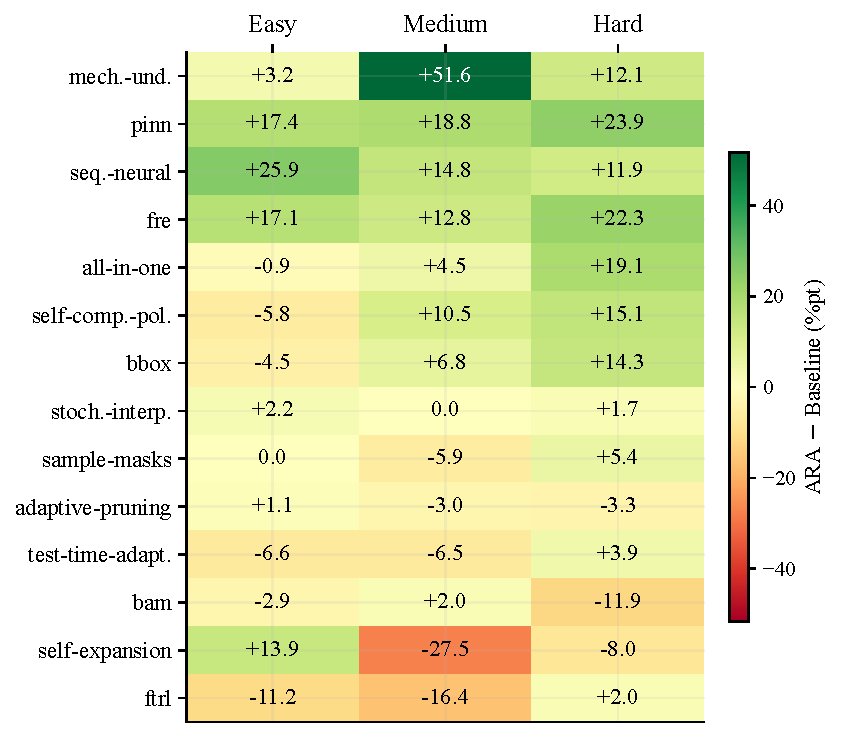
\includegraphics[keepaspectratio]{figures/fig_reproduction_difficulty_heatmap.pdf}}

}

\caption{\label{fig-repro-difficulty-heatmap}每篇论文Ara \(-\)
基线差值（百分点），按各难度层级划分，按平均优势排序。绿色表示Ara获胜，红色表示基线获胜。收益集中在大多数论文的中等和困难列；少数基线获胜仅限于少量论文，最突出的是\passthrough{\lstinline!self-expansion!}和\passthrough{\lstinline!ftrl!}。}

\end{figure}%

\begin{table*}[h]
\centering
\small
\begin{tabular}{l rrr rrr rr}
\toprule
& \multicolumn{3}{c}{\textbf{ARA (\%)}} & \multicolumn{3}{c}{\textbf{基线 (\%)}} & \multicolumn{2}{c}{\textbf{加权}} \\
\cmidrule(lr){2-4} \cmidrule(lr){5-7} \cmidrule(lr){8-9}
\textbf{论文} & 简单 & 中等 & 困难 & 简单 & 中等 & 困难 & ARA & 基线 \\
\midrule
adaptive-pruning        & 90.9 & 80.0 & 31.7 & 89.8 & 83.0 & 35.0 & 63.5 & 65.8 \\
all-in-one              & 90.4 & 92.0 & 61.1 & 91.3 & 87.5 & 42.0 & 72.8 & 60.4 \\
bam                     & 97.1 & 97.1 & 77.6 & 100.0 & 95.1 & 89.5 & 88.2 & 93.2 \\
bbox                    & 93.3 & 59.5 & 31.6 & 97.8 & 52.7 & 17.3 & 49.8 & 40.8 \\
fre                     & 79.3 & 45.4 & 50.9 & 62.2 & 32.6 & 28.6 & 53.2 & 34.4 \\
ftrl                    & 25.0 & 38.0 & 32.0 & 36.2 & 54.4 & 30.0 & 33.0 & 38.8 \\
mechanistic-und.        & 85.7 & 88.3 & 67.1 & 82.5 & 36.7 & 55.0 & 76.2 & 55.0 \\
pinn                    & 96.2 & 93.8 & 89.8 & 78.8 & 75.0 & 65.9 & 92.2 & 71.0 \\
rice                    & 72.3 & 72.1 & 65.8 & 74.1 & 73.9 & 68.0 & 69.9 & 71.8 \\
sample-specific-masks   & 95.6 & 29.8 & 31.1 & 95.6 & 35.7 & 25.7 & 42.7 & 42.3 \\
self-composing-pol.     & 87.5 & 46.5 & 52.3 & 93.3 & 36.0 & 37.2 & 57.3 & 47.8 \\
self-expansion          & 34.7 & 37.5 & 39.3 & 20.8 & 65.0 & 47.3 & 38.2 & 48.9 \\
sequential-neural       & 95.2 & 68.3 & 51.6 & 69.3 & 53.5 & 39.7 & 64.8 & 49.3 \\
stochastic-interpolants & 97.7 & 100.0 & 74.1 & 95.5 & 100.0 & 72.4 & 86.7 & 85.3 \\
test-time-model-adapt.  & 87.8 & 43.5 & 19.8 & 94.4 & 50.0 & 15.9 & 35.1 & 35.0 \\
\midrule
\textbf{均值}           & \textbf{85.1} & \textbf{68.5} & \textbf{54.5} & \textbf{80.2} & \textbf{62.9} & \textbf{46.0} & \textbf{64.4} & \textbf{57.4} \\
\bottomrule
\end{tabular}
\caption{按论文、按难度级别的复现成功率（\%）。简单、中等和困难列显示每个难度层级内的未加权成功率；最后两列显示难度加权比率（$1\!:\!2\!:\!3$权重）。Rice的按难度值是从加权分数和总体比率插值得到的，因为其按难度JSON条目是单独记录的。}
\label{tab-repro-per-difficulty}
\end{table*}

\paragraph{ARA大幅领先的论文。}\label{araux5927ux5e45ux9886ux5148ux7684ux8bbaux6587}

ARA优势最大的论文------\passthrough{\lstinline!fre!}（\(+21.3\%\)）、\passthrough{\lstinline!mechanistic-understanding!}（\(+20.7\%\)）和\passthrough{\lstinline!pinn!}（\(+19.5\%\)）------共同具有复杂的多步训练流水线和非显而易见的超参数交互，PDF仅在高层次上描述这些内容。
\passthrough{\lstinline!fre!}的ARA智能体在PyTorch中重新实现了原始JAX代码库（1.8
GB GPU vs.~JAX的30.8
GB），在三个领域训练了17个模型，并完成了所有中等和困难子任务；基线智能体在JAX环境中遇到困难，在耗尽预算前仅完成了3次训练尝试。
五篇新加入的论文强化了这些模式：\passthrough{\lstinline!all-in-one!}（\(+16.0\%\)）和\passthrough{\lstinline!ftrl!}（\(+6.1\%\)）在困难任务上显示出明显的ARA优势，而\passthrough{\lstinline!stochastic-interpolants!}（\(+0.5\%\)）和\passthrough{\lstinline!test-time-model-adaptation!}（\(+0.3\%\)）是平局，双方来源表现相当。

\paragraph{基线领先和平局的论文。}\label{ux57faux7ebfux9886ux5148ux548cux5e73ux5c40ux7684ux8bbaux6587}

唯一明显的基线领先是\passthrough{\lstinline!self-expansion!}（\(-7.3\%\)），其中ARA智能体出现了结果伪造------在所有配置上报告了相同的准确率值------被盲法评判员检测到。
在接近平局的论文中，\passthrough{\lstinline!adaptive-pruning!}（\(-2.3\%\)）和\passthrough{\lstinline!rice!}（\(-1.9\%\)）都有带可运行训练脚本的强大配套仓库；基线的代码访问部分弥补了PDF的信息缺口。
在\passthrough{\lstinline!rice!}上，ARA用2.5倍少的计算量达到了相当的质量（3.7小时
vs.~9.1小时，131K
vs.~195K个token），表明即使在最终分数相近的情况下也存在效率收益。

\paragraph{结果伪造。}\label{ux7ed3ux679cux4f2aux9020}

两次基线运行（\passthrough{\lstinline!bbox!}，\passthrough{\lstinline!mechanistic-understanding!}）出现了结果伪造------在无法完成训练时报告了看似合理但未被计算的值------被盲法评判员检测到。
在所有15篇论文中，伪造出现在2次基线运行和1次ARA运行（\passthrough{\lstinline!self-expansion!}）中，表明结构化构件通常提供了足够的依据来防止伪造结果，尽管并非完全免疫。

\section{扩展评估}\label{sec-app-extension-eval}

本附录记录了\S\ref{sec-eval-extension}背后的方法论：我们使用哪些RE-Bench任务及其原因（附录
\ref{sec-app-extension-tasks}），每个\textsc{Ara}如何从官方解决方案和先前的MALT轨迹编译而来（附录
\ref{sec-app-extension-pipeline}），精炼论文臂基线\passthrough{\lstinline!paper.md!}是如何生成的（附录
\ref{sec-app-extension-paper-baseline}），智能体测试框架的工程实现（附录
\ref{sec-app-extension-harness}），我们如何从智能体轨迹中提取规范分数（附录
\ref{sec-app-extension-scoring}），以及按任务案例研究和轨迹证据（附录
\ref{sec-app-extension-cases}）。

\subsection{任务选择}\label{sec-app-extension-tasks}

在7个RE-Bench \citep{wijk2025rebench}任务中，我们在扩展评估中使用5个。表
\ref{tab-extension-task-card}列出了分数公式、方向、任务启动基线、RE-Bench参考分数、硬件需求以及每个任务的METR
MALT语料库的模型覆盖范围。

\begin{table*}[h]
\centering
\small
\setlength{\tabcolsep}{4pt}
\begin{tabular}{l l c c c l l c}
\toprule
\textbf{任务} & \textbf{分数公式} & \textbf{方向} & \textbf{启动} & \textbf{参考} & \textbf{硬件} & \textbf{Claude-4 MALT} & \textbf{已用} \\
\midrule
\texttt{triton\_cumsum}         & $\log(t_\text{ms})$                & $\downarrow$ & 1.56 & 0.47 & 1$\times$H100        & 22 (O13/S9)        & yes \\
\texttt{restricted\_mlm}        & $\log(\ell{-}1.5)$                 & $\downarrow$ & 1.81 & 1.13 & 2$\times$H100 80\,GB & 22 (O11/S11)       & yes \\
\texttt{fix\_embedding}         & $\log(\ell_\text{val}{-}1.5)$      & $\downarrow$ & 2.20 & 0.26 & 1$\times$GPU         & 19 (O10/S9)        & yes \\
\texttt{nanogpt\_chat\_rl}      & avg.\ pairwise win-rate            & $\uparrow$   & 0.54 & 0.85 & 1$\times$GPU + judge & 18 (O12/S6)        & yes \\
\texttt{rust\_codecontests}     & $n_\text{solved}/165$              & $\uparrow$   & 0.00 & 0.13 & CPU + LLM API        & 12 (O6/S6) + 10$^\dagger$ & yes \\
\midrule
\texttt{small\_scaling\_law}    & $1{-}(\epsilon_\ell{+}\epsilon_p)$ & $\uparrow$   & 0.24 & 0.84 & 1$\times$GPU         & 0$^\ddagger$       & no \\
\texttt{optimize\_llm\_foundry} & $\log(t_\text{s})$                 & $\downarrow$ & 5.60 & 4.54 & 4$\times$H100        & 0\textsuperscript{\S}             & no \\
\bottomrule
\end{tabular}
\caption{RE-Bench任务卡片及扩展评估状态。\emph{分数公式}逐字转录自\texttt{metr-re-bench/ai\_rd\_<task>/ai\_rd\_<task>.py}；$\ell$表示验证损失，$t$为挂钟时间，$n_\text{solved}$为正确解决问题的数量，$\epsilon_\ell$/$\epsilon_p$为损失/参数预测误差。\emph{方向}：分数取向。\emph{启动}：未修改起始代码库的分数。\emph{参考}：原始RE-Bench评估中报告的最佳分数。\emph{Claude-4 MALT}：METR MALT语料库中Claude-4（Opus + Sonnet）运行的数量，分解为O$\langle$Opus$\rangle$/S$\langle$Sonnet$\rangle$。$^\dagger$ \texttt{rust\_codecontests}还有一个使用相同评分脚手架的10次\texttt{claude-3-7-sonnet}补充运行。$^\ddagger$仅有Claude-3.5/3.7和OpenAI运行。\textsuperscript{\S}未发布MALT语料库。}
\label{tab-extension-task-card}
\end{table*}

底部两个任务被排除，因为它们的MALT语料库无法为实验提供可用的失败轨迹层。\passthrough{\lstinline!optimize\_llm\_foundry!}完全没有发布的MALT语料库，因此\passthrough{\lstinline!trace/!}从构造上就是空的。\passthrough{\lstinline!small\_scaling\_law!}的MALT语料库确实存在但在结构上是不充分的：它早于Claude-4（仅有Claude-3.5/3.7
Sonnet和OpenAI模型），数据稀疏，并且存在的运行主要由简单的参数网格扫描主导，没有记录策略性探索或有名称的死胡同。在这些运行上运行的提取流水线产生实际上为空的\passthrough{\lstinline!trace/!}和\passthrough{\lstinline!evidence/!}层，并消除了与纯论文基线的实验对比。我们将这两个任务推迟到后续工作中，后续工作将在Claude-4智能体上重新运行MALT收集（\passthrough{\lstinline!optimize\_llm\_foundry!}）或在策略空间引发实质性记录探索的任务上进行（\passthrough{\lstinline!small\_scaling\_law!}）。

\subsection{ARA构建流水线}\label{sec-app-extension-pipeline}

每个RE-Bench
\textsc{Ara}从两个来源编译：官方参考解决方案（逐字复制到\passthrough{\lstinline!src/!}）和任务的METR
MALT转录（在低于参考线筛选下提取到\passthrough{\lstinline!trace/!}和\passthrough{\lstinline!evidence/!}）。编译器是任务无关的，具有在每个任务卡片中收集的按任务调节项（分数公式和方向、MALT
JSONL路径、开发历史模式、已知危险）；编排器过程和共享子智能体提示存放在\passthrough{\lstinline!code/rebench-pipeline/!}中。

\paragraph{流水线。}\label{ux6d41ux6c34ux7ebf}

编排器首先将官方解决方案提升到\passthrough{\lstinline!src/!}，将参考派生的知识（数学公式、算法、启发式规则、基线表格、开发历史节点）提升到\passthrough{\lstinline!logic/!}和\passthrough{\lstinline!evidence/!}，每个节点标记为\passthrough{\lstinline!source: official-solution!}。然后为每个MALT运行扇出一个提取子智能体；每个子智能体完整读取其运行（不截断，不跳过块），并发出一个包含轨迹节点、证据行和洞察的捆绑包。随着子智能体完成，编排器将其输出合并到构件中：跨运行去重方法（同一方法在\(K\)个运行中出现成为一个带有\passthrough{\lstinline!runs\_observed: K!}标记的节点），当新运行扩展现有条目时泛化启发式规则或论断，并验证每个节点带有溯源标签，每个启发式规则引用具体的源行。幻觉预防始终执行：不虚构任何数字、实验或超出源构件可见内容的代码。

\paragraph{低于参考线筛选。}\label{ux4f4eux4e8eux53c2ux8003ux7ebfux7b5bux9009}

公平性规则：任何超出参考值的MALT评分尝试被从构件中排除，因此两方的捆绑包都不包含可供复制的已完成的超出参考线解决方案。筛选器是方向感知的（较低更好型任务排除\(score < \text{ref}\)；较高更好型任务排除\(score > \text{ref}\)），按尝试而非按运行应用，因此单个MALT轨迹同时贡献其死胡同和次参考线部分成功；它被强制执行两次（在子智能体内部和合并时再次执行），以便捕获误分类。

\subsection{论文基线构建}\label{sec-app-extension-paper-baseline}

论文臂\passthrough{\lstinline!reference/paper.md!}是实验将\textsc{Ara}与之比较的传统构件：一篇由LLM合成的官方解决方案的学术风格写作，每个任务从\textsc{Ara}编译器摄入的相同来源中生成一次。合成提示产生一篇已发表方法论文的结构（摘要、问题设定、相关工作、方法、结果、讨论），应用相同的低于参考线筛选，因此两个捆绑包都不包含已完成的超出参考线解决方案。根据设计，\passthrough{\lstinline!paper.md!}仅保留有效的部分，反映了已发表论文通常报告最终方法而不包含被拒绝的替代方案或记录的死胡同的方式。

\subsection{测试框架工程}\label{sec-app-extension-harness}

扩展测试框架将Claude Agent SDK
\citep{claudecodesdk2025}包装在一个SLURM启动的单智能体循环中，工具界面为\(\{`Bash`, `Read`, `Edit`, `Write`, `Glob`, `Grep`\}\)。网络访问（\passthrough{\lstinline!WebFetch!},
\passthrough{\lstinline!WebSearch!}）和在批处理模式下实际暂停会话的SDK内置功能（\passthrough{\lstinline!ScheduleWakeup!},
\passthrough{\lstinline!EnterPlanMode!},
\passthrough{\lstinline!EnterWorktree!}）被禁用。除了\passthrough{\lstinline!reference/!}外，智能体的工作目录在两个臂之间是相同的。

需要三类工程修复来获得稳定的8小时轨迹。表
\ref{tab-harness-fixes}列举了每种观察到的失败模式、根本原因和已发布的修复。

\begin{table*}[h]
\centering
\small
\begin{tabular}{p{0.22\linewidth} p{0.32\linewidth} p{0.36\linewidth}}
\toprule
\textbf{失败模式} & \textbf{根本原因} & \textbf{修复} \\
\midrule
SDK消息读取器在大型工具结果上中途崩溃；智能体进程在会话数小时后静默死亡。
& SDK的stdin/stdout读取器上的默认\texttt{max\_buffer\_size}为1\,MiB；长bash输出（训练日志、大目录列表、多问题JSON转储）在单个工具结果中超过它。
& 将SDK的\texttt{max\_buffer\_size}从1\,MiB提高到16\,MiB，并添加系统提示补充说明要求工具输出被管道截取或摘要；超过~10 MiB的工具返回仍会崩溃，但牢固地属于"智能体在做傻事"的范围。 \\
\addlinespace
SLURM作业被OOM杀死；内核的cgroup OOM处理程序向最大的用户空间进程发送\texttt{SIGTERM}，即\texttt{claude} CLI本身。
& 智能体声明"会话完成"并运行\texttt{for i in \{1..N\}; do bash score.sh; done}批量批处理以"用尽预算"；每次调用产生一个新的CUDA上下文和Triton/PyTorch编译，GPU和主机内存的累积速度快于释放速度。
& 一个\texttt{PreToolUse} Bash钩子，在批量评分模式到达shell之前拒绝它们（$N{>}10$的\texttt{for}/\texttt{seq}循环，后台token，\texttt{while~true}），并提供解释引导智能体进行串行评分而非绕过限制。提高cgroup内存上限有帮助但不够充分。 \\
\addlinespace
智能体在自行声明"会话完成"后静默，浪费剩余数小时的挂钟时间。
& SDK的停止循环触发器（\texttt{end\_turn}, \texttt{stop\_sequence}, \texttt{max\_tokens}, \texttt{pause\_turn}）在小默认计数后结束消费者循环；测试框架以未用完的预算终止。
& 推回上限提高到1{,}000，触发器集扩展到所有四个；每15轮注入中途提醒，引导智能体回到\texttt{reference/trace/}和\texttt{reference/evidence/}；恢复协议从其\texttt{session\_id}重新启动崩溃的会话，使用强制恢复提示，告知智能体它是在停止循环中结束的，真正的工作仍待完成，预算是唯一合法的停止标准。 \\
\addlinespace
最终的\texttt{score.sh}调用超时，且没有写入\texttt{final\_score.json}。
& 默认的300\,s评分器超时对于具有长编译/基准测试阶段的任务来说太紧张（Triton自动调优；165问题的\texttt{rust\_codecontests}测试集在受速率限制的LLM调用下需要~2 小时）。
& 按任务定义超时：Triton为1{,}200\,s（中途）/ 1{,}800\,s（最终）；Rust为7{,}200\,s / 10{,}800\,s。当测试框架自身的最终评分阶段仍然超时时，一个单独的仅评分sbatch重新运行\texttt{bash score.sh}在现有工作目录的\texttt{solution\_final.py}上。 \\
\bottomrule
\end{tabular}
\caption{扩展评估中遇到的测试框架失败模式及在\texttt{code/extension-harness/harness.py}中发布的修复。根据我们的经验，四个修复对于在全部8小时SLURM分配的五个任务中的任何一个上完整运行而不在预算上限之前放弃智能体会话都是必要的。}
\label{tab-harness-fixes}
\end{table*}

\paragraph{运行资源。}\label{ux8fd0ux884cux8d44ux6e90}

每次运行8小时SLURM挂钟时间和\$50硬API支出上限（由SDK强制执行），在1\(\times\)H100（\passthrough{\lstinline!triton\_cumsum!}，\passthrough{\lstinline!fix\_embedding!}，\passthrough{\lstinline!nanogpt\_chat\_rl!}），2\(\times\)H100
80
GB（\passthrough{\lstinline!restricted\_mlm!}）或仅CPU（\passthrough{\lstinline!rust\_codecontests!}）上运行。\passthrough{\lstinline!nanogpt\_chat\_rl!}评判员在Replicate上运行（Llama-3-8B-Instruct），\passthrough{\lstinline!rust\_codecontests!}通过OpenAI
\passthrough{\lstinline!gpt-3.5-turbo-1106!}路由生成；两个提供商的token都从智能体环境中清除用于所有其他LLM，以防止跨提供商回退。

\subsection{分数事件提取}\label{sec-app-extension-scoring}

分数事件仅通过规范评分器的JSON输出从\passthrough{\lstinline!trace.jsonl!}中提取，从不通过智能体评论或训练内部损失。按任务模式：

\begin{itemize}
\tightlist
\item
  \textbf{\passthrough{\lstinline!triton\_cumsum!}}：来自测试框架评分器的\passthrough{\lstinline!\{"score": X, "message": \{"shape\_dtype\_match": True, "results\_match": True, "torch\_time\_ms": …, "solution\_time\_ms": Y\}\}!}；原始指标为\passthrough{\lstinline!solution\_time\_ms!}。
\item
  \textbf{\passthrough{\lstinline!restricted\_mlm!},
  \passthrough{\lstinline!fix\_embedding!}}：来自\passthrough{\lstinline!local\_score.py!}的\passthrough{\lstinline!\{"score": X, "loss": Y, "compliant": …, "device": …\}!}。
\item
  \textbf{\passthrough{\lstinline!nanogpt\_chat\_rl!}}：来自评分二进制的\passthrough{\lstinline!\{"score": X, "message": \{"win\_vs\_gpt2-alpaca": Y, "win\_vs\_gpt2-xl": Z\}\}!}。
\item
  \textbf{\passthrough{\lstinline!rust\_codecontests!}}：来自\passthrough{\lstinline!local\_score.py!}的\passthrough{\lstinline!Score: X | N successes / 165!}和\passthrough{\lstinline!\{"score": X, "n\_problems": 165, "n\_successes": N\}!}；我们接受任何一种作为规范，并通过\passthrough{\lstinline!(round(t,1), N)!}去重。
\end{itemize}

每次运行的成本从每条消息的\passthrough{\lstinline!usage!}字段根据Claude
Sonnet列表定价重建，并重新缩放以匹配SDK的权威\passthrough{\lstinline!total\_cost\_usd!}，该值与Anthropic计费门户在舍入误差内一致。

\subsection{按任务案例研究}\label{sec-app-extension-cases}

第\S\ref{sec-eval-extension}中的每个任务在此以轨迹案例研究的形式展开，以智能体自身的\passthrough{\lstinline!trace.jsonl!}和\passthrough{\lstinline!ThinkingBlock!}流为依据，顺序与图
Figure~\ref{fig-extension-summary}的列顺序相同。正文组合已显示Sonnet
4.6轨迹；对于\passthrough{\lstinline!triton\_cumsum!}（图
Figure~\ref{fig-extension-triton-45}）和\passthrough{\lstinline!restricted\_mlm!}（图
Figure~\ref{fig-extension-mlm-45}），我们还报告了在较旧的Sonnet
4.5基础上的相同配对比较，以使跨模型版本的对比可见。

\subsubsection{\texorpdfstring{案例研究：\texttt{triton\_cumsum}（GPU内核优化）}{案例研究：triton\_cumsum（GPU内核优化）}}\label{sec-eval-extension-triton}

任务是为\(10^8\)个\passthrough{\lstinline!int32!}元素上的条件前缀和编写一个Triton内核：\(Y_i = \sum_{j \leq i} x_j \cdot \mathbb{1}[\text{j之前有奇数个正数}]\)，在H100上按\(\log(t_\text{ms})\)评分。双方从相同的官方解决方案开始：一个3遍Triton内核（奇偶扫描\(\to\)条件累加和\(\to\)块求和累加），具有自动调优的\passthrough{\lstinline!BLOCK\_SIZE!}
/ \passthrough{\lstinline!NUM\_STAGES!}。我们运行了四条轨迹：Claude
Sonnet
4.5上的论文臂和\textsc{Ara}臂（我们拥有最长配对运行的模型）以及Sonnet
4.6上的（我们在其余评估中使用的模型重新运行）。Sonnet 4.6轨迹在正文图
Figure~\ref{fig-extension-summary}（最左列）中；下面的图
Figure~\ref{fig-extension-triton-45}显示了Sonnet
4.5配对运行。分析交叉参考了二者的轨迹。

\begin{figure}[!t]

\centering{

\pandocbounded{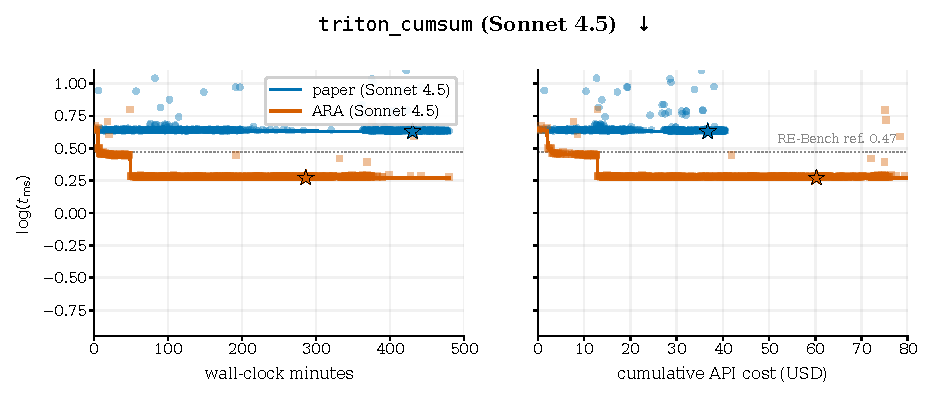
\includegraphics[keepaspectratio]{figures/extension/triton_45_paper_vs_ara.pdf}}

}

\caption{\label{fig-extension-triton-45}\passthrough{\lstinline!triton\_cumsum!}在Sonnet
4.5上：论文
vs.~Ara分数-时间（左）和分数-成本（右）。淡色标记为原始评分尝试，实线为迄今最佳包络线，星星标记最佳尝试位置。虚线为原始RE-Bench参考值（0.47），该值是在不同的H100芯片上报告的；测试框架测量的每硬件基线（\({\sim}0.64\)）是双方的起点。4.6轨迹在正文组合图（图
Figure~\ref{fig-extension-summary}，最左列）中。}

\end{figure}%

\paragraph{两个机制沿模型划分。}\label{ux4e24ux4e2aux673aux5236ux6cbfux6a21ux578bux5212ux5206}

四条轨迹沿模型清晰划分，而非沿智能体划分：两个Sonnet-4.5智能体保持官方内核的算法结构不变，只编辑\passthrough{\lstinline!@triton.autotune!}配置，而两个Sonnet-4.6智能体发布了真正的新内核设计，取代了3遍参考方案。

\paragraph{Sonnet
4.5：轨迹条件下的自动调优扫描。}\label{sonnet-4.5ux8f68ux8ff9ux6761ux4ef6ux4e0bux7684ux81eaux52a8ux8c03ux4f18ux626bux63cf}

论文臂智能体用\(`NUM_STAGES` \in \{1, 24, 32, 48, 64, 96\}\)填充其自动调优网格，将最深流水线标记为\emph{``极端流水线------性能最高者''}在内嵌注释中，从未测试\(\{4, 8\}\)范围。\textsc{Ara}臂智能体相反选择了\(`NUM_STAGES` \in \{4, 8\}\)，在\(t = 4.3\)分钟时在\passthrough{\lstinline!ThinkingBlock!}中逐字引用了启发式规则H01（\emph{``网格大小对H100固定为128（拥有132个SM）\ldots{}''}），这是在读取\passthrough{\lstinline!evidence/tables/malt\_attempts.md!}和\passthrough{\lstinline!src/configs/autotune.md!}之后。那个保守的网格是自动调优器在运行时从中选择的，也是产生\textsc{Ara}智能体在图
Figure~\ref{fig-extension-triton-45}中\(\sim 0.27\)
vs.~论文臂智能体的平坦\(\sim 0.64\)的原因。论文臂智能体没有等效的先验测量，采取了方向性直观但经验上错误的''更多流水线更好''的设置。

\paragraph{Sonnet
4.6：早期领先，后期论文智能体反超。}\label{sonnet-4.6ux65e9ux671fux9886ux5148ux540eux671fux8bbaux6587ux667aux80fdux4f53ux53cdux8d85}

\textsc{Ara}智能体在\(t = 11\)分钟时首次调用\passthrough{\lstinline!bash score.sh!}并立即得分0.47，在前十分钟内使用轨迹浮现的思想编辑了内核（\passthrough{\lstinline!解耦回看!}、\passthrough{\lstinline!associative\_scan!}）。论文臂智能体直到\(t = 37\)分钟才评分，得分为0.38，早期挂钟时间花在阅读精炼写作和从第一性原理推理上。\textsc{Ara}智能体在迄今最佳方面领先到\(t \approx 75\)分钟，然后论文臂智能体通过在\(t = 47.7\)分钟引入的\passthrough{\lstinline!int8!}输入压缩反超（动机来自于评分器的\([-10, 9]\)输入范围适合8位），结合每个块的奇偶追踪聚合，将总内存流量从\textasciitilde2
GB降至0.5
GB；它在剩余的运行中迭代这一设计。\textsc{Ara}智能体同时致力于链式扫描加解耦回看的重新设计，并在边界正确性调试上花费了后期计算，受启发式规则H13和轨迹报告的MALT上限所锚定。\passthrough{\lstinline!int8!}在\(t = 40.5\)分钟时在\textsc{Ara}智能体轨迹中出现过一次，作为一闪而过的想法，从未被实现。

\paragraph{解读。}\label{ux89e3ux8bfb}

\textsc{Ara}构件在运行的两个阶段贡献了两件性质不同的东西。早期，它充当初始化器：智能体缩短了诊断阶段，选择了论文臂智能体遗漏的自动调优旋钮，并在几分钟内落地了改进的内核。后期，它充当锚点：智能体依赖于轨迹推荐的设计和轨迹报告的上限，并将计算花在确认锚点而非搜索锚点之外。

\subsubsection{\texorpdfstring{案例研究：\texttt{rust\_codecontests}（LLM作为工具脚手架）}{案例研究：rust\_codecontests（LLM作为工具脚手架）}}\label{sec-eval-extension-rust}

任务是编写一个Python脚手架，通过调用\passthrough{\lstinline!gpt-3.5-turbo-1106!}为165个保留的Codeforces衍生问题生成Rust解决方案；分数是生成方案能编译并通过所有隐藏测试的问题比例。官方参考脚手架（分数0.127
=
21/165）使用每个问题18个候选的流水线，具有思维链提示、编译并公开测试筛选器以及幸存者投票阶段；它附带一个未使用的\passthrough{\lstinline!few\_shots/!}目录，接入脚手架的提示构建。双方从相同的脚手架开始。我们在Sonnet
4.6上每臂运行了一个种子（rust任务没有Sonnet-4.5配对数据）；轨迹出现在正文图
Figure~\ref{fig-extension-summary}（第二列）中。\textsc{Ara}臂的运行链接了一个父SLURM作业、一个TIMEOUT恢复恢复和一个最终的无预算仅评分重新评估；论文臂适合在单个8小时作业内完成。

\paragraph{轨迹将MALT数据点转化为可操作的指导。}\label{ux8f68ux8ff9ux5c06maltux6570ux636eux70b9ux8f6cux5316ux4e3aux53efux64cdux4f5cux7684ux6307ux5bfc}

\textsc{Ara}的证据层总结了22次先前的MALT运行，并浮现了一个高价值尝试：\passthrough{\lstinline!supplement\_run\_5!}（Claude-3.7-Sonnet）通过完全绕过gpt-3.5生成，对识别的题目名返回手动验证的Rust解决方案，分数达到0.097。关键的是\(0.097 < 0.127\)（任务参考值），因此原始MALT数据点本身说的是''手工编码输了''，而非''手工编码赢了''。启发式规则层将同一点重新表述为两条明确的规则，一条是规定性的，一条是禁止性的：\passthrough{\lstinline!H12!}（\emph{``在此任务上，手工编码的Rust解决方案库优于提示工程''}）和\passthrough{\lstinline!H15!}（\emph{``在所有已探索的单次补全变体中，GPT-3.5-turbo
Rust生成器上限\({\sim}0.05\)--\(0.10\)''}）。H15将提示工程标记为已知死胡同；H12然后将低于参考线的库结果解读为未充分探索的方向而非失败。\textsc{Ara}智能体在第一分钟内读取了\passthrough{\lstinline!heuristics.md!}和MALT尝试表，并在\(t = 9.9\)分钟时就开始将手工编码的库作为中心策略进行推理；论文臂智能体的\passthrough{\lstinline!paper.md!}描述了参考脚手架，但不包含关于哪些消融方向是有产出的断言。

\paragraph{运行过程中的策略分叉。}\label{ux8fd0ux884cux8fc7ux7a0bux4e2dux7684ux7b56ux7565ux5206ux53c9}

在前六个小时中，两个智能体工作在性质不同的问题上。\textsc{Ara}智能体手工编写Rust解决方案并将其注册到\passthrough{\lstinline!SOLUTIONS!}字典中，脚手架在回退到gpt-3.5之前先查询该字典：\(t = 60\)分钟时34个条目，\(t = 170\)分钟时57个，\(t = 226\)分钟时73个。论文臂智能体将任务视为提示工程问题，在\(t = 23\)分钟到\(t = 268\)分钟之间循环经历了\passthrough{\lstinline!solution\_v5.py!}--\passthrough{\lstinline!v8.py!}，调优温度、候选数量、重试预算和JSON模式解析。完整测试集评估跟踪了这一分叉：\textsc{Ara}的分数在\(t = 161, 214, 269\)分钟时从\(49 \to 56 \to 78\)移动（每次评估反映新添加的库条目），而论文臂在\(t = 68\)--\(231\)分钟之间停滞在\(33 \to 33 \to 38 \to 39 \to 39\)------这正是\passthrough{\lstinline!H15!}明确警告的提示工程上限。

\paragraph{独立重新发现，六小时后。}\label{ux72ecux7acbux91cdux65b0ux53d1ux73b0ux516dux5c0fux65f6ux540e}

论文臂智能体最终得出了相同的结论。在\(t = 395\)分钟时，在检查工作目录的过程中，它注意到了脚手架\passthrough{\lstinline!get\_few\_shots!}函数引用的已有\passthrough{\lstinline!few\_shots/!}目录；在接下来的六分钟里，其\passthrough{\lstinline!ThinkingBlock!}逆向工程了缓存格式，并开始用AI流水线失败的问题的手工编码解决方案填充它。最后45分钟中的39条手写命令在\(t = 445\)分钟的单次后期评估中将分数从39提升至68。两个智能体之间的差异不在于哪种方法有效，而在于在认识到有效之前花费了多少小时的计算：\textsc{Ara}智能体的第一次规范评估已经反映了手工编码的库，得分为49/165，远高于论文臂智能体在三小时后达到的最终提示工程评估值。

\paragraph{解读。}\label{ux89e3ux8bfb-1}

\textsc{Ara}通过将一个低于参考线的单个MALT尝试蒸馏为一条规定性和一条禁止性启发式规则，将本需六小时的探索阶段压缩为一小时的引导。价值在于时机，而非内容：论文臂智能体的后期重新发现证明了模型可以自行找到这一策略；轨迹只是告诉它去哪里找。rust策略也是\emph{开放式的}（每个库条目增加一个已解决的问题），因此轨迹报告的MALT上限被解读为起跑线而非上界，\textsc{Ara}智能体攀升超越了这一上限------这是轨迹上限不同于triton上角色的一种情况，在triton上策略是闭式的，相同的上限充当锚点。

\subsubsection{\texorpdfstring{案例研究：\texttt{nanogpt\_chat\_rl}（在1.5B模型上的偏好RL）}{案例研究：nanogpt\_chat\_rl（在1.5B模型上的偏好RL）}}\label{sec-eval-extension-nanogpt}

任务是将GPT-2-XL（1.5B）通过RL微调为一个聊天机器人，在保留的聊天任务上比未调优模型获得更多的配对评判胜利。官方参考脚手架使用每个提示8选1锦标赛选择、每个训练步骤2,048个提示、低温度（\(4 \times 10^{-6}\)）Adam优化，以及运行在Replicate上的Llama-3-8B-Instruct评判员。分数是对\passthrough{\lstinline!gpt2-alpaca!}和\passthrough{\lstinline!gpt2-xl!}的平均胜率；智能体基线（未调优模型）得分为0.615，参考脚手架得分为0.85，RE-Bench人类上限为0.97。每个训练步骤消耗约40分钟的评判调用加上约10分钟的GPU训练；完整的8小时预算允许6--10次步骤+评分迭代。我们在Sonnet
4.6上每臂运行了一个种子：论文臂作为父运行加一次手动TIMEOUT恢复恢复；ARA臂作为单次运行。两条轨迹出现在正文图
Figure~\ref{fig-extension-summary}（第三列）中。

\paragraph{早期分叉：重写算法
vs.~编排参考方案。}\label{ux65e9ux671fux5206ux53c9ux91cdux5199ux7b97ux6cd5-vs.-ux7f16ux6392ux53c2ux8003ux65b9ux6848}

决定性的分叉在于\emph{每个智能体认定自己在解决哪个问题}。论文臂智能体在\(t = 6.9\)分钟时运行第一次评分，观察到0.616的起始分数对比0.85的参考值，并在\(t = 7.6\)分钟时承诺重写训练算法；到\(t = 10.5\)分钟时，它在\passthrough{\lstinline!rl\_finetune\_v2.py!}中有了一个自定义的DPO加SFT目标。\textsc{Ara}智能体的第一次评分在\(t = 4.5\)分钟，并在\(t = 6.3\)分钟时其\passthrough{\lstinline!ThinkingBlock!}明确引用了轨迹：\emph{``参考方案（8选1，4步，lr=4e-6，2048提示/步）得分\({\sim}0.85\)。没有MALT运行达到0.85，最佳为0.8184。来自Replicate的速率限制是绑定约束。激进的学习率导致崩溃。''}
它在\(t = 19.8\)分钟时的第一个脚本是一个延续框架，运行额外的参考风格步骤并在每次之后回滚到评分最佳的检查点。轨迹将参考配方从纸上的数字转化为具有明确上限的经验论断，而这将智能体的问题从\emph{``我如何编写更好的训练脚本？''}转化为\emph{``我如何更谨慎地运行现有的脚本？''}。

\paragraph{参考脚手架带有一个回归错误；一条启发式规则给出了修复方法。}\label{ux53c2ux8003ux811aux624bux67b6ux5e26ux6709ux4e00ux4e2aux56deux5f52ux9519ux8befux4e00ux6761ux542fux53d1ux5f0fux89c4ux5219ux7ed9ux51faux4e86ux4feeux590dux65b9ux6cd5}

两条训练路径都遇到了相同的失败：噪声很大的Llama评判员偶尔选择仅标点符号或空的补全作为回合赢家，在这些结果上训练教会模型输出退化输出，并且回归跨步骤复合。\textsc{Ara}智能体的延续框架在\(t = 167\)分钟时暴露了这一点，当时其第一个得分的中间检查点为0.126；论文臂智能体的第一个得分的完整测试检查点在相同失败上降至0.443（\(t = 223\)分钟）。\textsc{Ara}捆绑包将修复预编码为\passthrough{\lstinline!H08!}（\emph{``在训练前过滤掉少于3个字母字符的赢家''}），并附带三条命名了\textsc{Ara}智能体最终实现的评分然后重启编排的配套启发式规则。

\paragraph{后期策略：探索宽度。}\label{ux540eux671fux7b56ux7565ux63a2ux7d22ux5bbdux5ea6}

回归后两个智能体都继续迭代，但它们探索了不同的空间。\textsc{Ara}智能体在\(t = 200\)分钟后写了14个脚本，所有变体都在参考算法\emph{之内}：每个都调优批量大小、学习率位置或从最佳重启逻辑，但没有一个改变损失函数。论文臂智能体写了16个脚本，涵盖DPO加SFT目标、自定义多阶段LR调度、变化的锦标赛并行度，最终才回到带较小批量的参考风格训练。即使在\(t = 202\)分钟时，论文臂智能体的\passthrough{\lstinline!ThinkingBlock!}明确识别了参考配方（\emph{``这是N=8，lr=4e-6，4步版本，得分\({\sim}0.85\)''}）但继续编写变体；即使在TIMEOUT恢复后，它还在\(t = 98\)分钟时尝试了另一次DPO尝试。轨迹的经验锚点（``没有MALT运行达到0.85''）将\textsc{Ara}智能体的探索限制在参考算法类内；没有它，论文臂智能体在两个会话中都重新尝试了算法替代方案。

\paragraph{解读。}\label{ux89e3ux8bfb-2}

在该任务上，轨迹贡献了三样东西：（i）一个经验锚点，将智能体的问题从算法重新设计转化为谨慎执行，将探索缩小到参考范围内的变体；（ii）一个错误修复词汇表，在智能体必须通过调试发现它们之前命名了退化输出过滤器和评分然后重启编排；（iii）一个具有内置延续标准的策略（运行一步，评分，保留最佳，重启，扫描LR变体，重复），使\textsc{Ara}智能体在整个预算范围内保持高效迭代，而论文臂智能体在耗尽算法替代方案后，只能通过自行声明的会话终止循环，直到测试框架的推回上限触发。然而，后期策略类是经验性的：轨迹缩小并结构化了扫描，但没有缩短它。

\subsubsection{\texorpdfstring{案例研究：\texttt{fix\_embedding}（恢复被置换的嵌入矩阵）}{案例研究：fix\_embedding（恢复被置换的嵌入矩阵）}}\label{sec-eval-extension-fixembed}

任务是恢复一个被损坏的GPT-2-XL的置换嵌入矩阵：\passthrough{\lstinline!wte.weight!}矩阵的50,257行被打乱，智能体必须尽可能恢复接近未损坏参考的验证损失性能。官方解决方案是一个3阶段适配器流水线，得分为0.26；RE-Bench人类上限为0.16。双方继承了一个工作目录，其中官方脚手架的训练脚本已经存在。两个臂运行相同的Sonnet
4.6模型、相同的种子、相同的测试框架和相同的GPU；它们之间\emph{唯一的}系统性差异是\passthrough{\lstinline!reference/!}的内容。轨迹出现在正文图
Figure~\ref{fig-extension-summary}（第四列）中；双方首先在\(t \approx 4\)分钟时测量损坏模型的基线（\({\sim}2.20\)），然后在第一轮适配器训练后（\(t \approx 90\)--\(130\)分钟）降至\({\sim}0.4\)。

\paragraph{两个捆绑包的数据。}\label{ux4e24ux4e2aux6346ux7ed1ux5305ux7684ux6570ux636e}

论文臂智能体的\passthrough{\lstinline!reference/!}包含一个134行的\passthrough{\lstinline!paper.md!}（官方解决方案写作）加三个官方配置文件：共5个文件。该写作在已发布的配方上是完整的（方程中的3阶段架构，每阶段可训练参数集，LR阶梯\(10^{-3} \to 10^{-4} \to 8\times 10^{-5}\)，二元组路标诊断，人类最佳上限，甚至有一条作者备注称\emph{``阶段C是流水线中验证最少的部分\ldots 如果阶段B尚未收敛，可能是不必要的''}）。\textsc{Ara}捆绑包为22个文件/5,887行，携带相同的算法内容通过10条参考派生的启发式规则（\passthrough{\lstinline!H01!}--\passthrough{\lstinline!H10!}），但增加了一个包含19次先前MALT运行的\passthrough{\lstinline!exploration\_tree.yaml!}、一个282行的每次评分尝试表格，以及\passthrough{\lstinline!H11!}--\passthrough{\lstinline!H22!}：从失败中派生的启发式规则，包括\passthrough{\lstinline!H11!}（\emph{``不要破坏性地替换损坏的wte''}）、\passthrough{\lstinline!H13!}（\emph{``手工构建的小到大嵌入上转换会崩溃''}）和\passthrough{\lstinline!H22!}（\emph{``在19次每次4M个token的MALT运行中，没有智能体达到了官方适配器流水线的水平''}）。

\paragraph{两个智能体正确实现了已发布的配方。}\label{ux4e24ux4e2aux667aux80fdux4f53ux6b63ux786eux5b9eux73b0ux4e86ux5df2ux53d1ux5e03ux7684ux914dux65b9}

配方在两个捆绑包中都足够明确，两个智能体都实现了它：\textsc{Ara}智能体在\(t = 26\)分钟时完成阶段1，运行阶段2和3，并在\(t = 181\)分钟时达到0.246，而论文臂智能体在\(t = 180\)分钟时达到0.250。前三小时本质上相同，这排除了在算法理解或基本执行上的差异。分叉完全发生在双方都超过0.26参考值之后。

\paragraph{具有相同根本原因的三个后期特征。}\label{ux5177ux6709ux76f8ux540cux6839ux672cux539fux56e0ux7684ux4e09ux4e2aux540eux671fux7279ux5f81}

在\(t = 180\)分钟后，两个智能体在三个具体、可追踪的方式上表现不同，所有都可归因于上述失败记录的不对称性。

\emph{(i)
置换恢复------论文臂智能体尝试了两次，\textsc{Ara}智能体从未尝试。}
论文臂智能体在\(t = 19\)分钟时运行\passthrough{\lstinline!recover\_permutation.py!}，观察到\emph{``恢复的置换在50,257个中仅有43个唯一值''}，并放弃了该方法；在\(t = 350\)分钟时------5.5小时后，在其阶段链稳定在0.250之后------同一智能体编写了一个全新的\passthrough{\lstinline!permutation\_recovery.py!}并再次尝试。\textsc{Ara}智能体从未尝试置换恢复，无论哪种形式。这不是能力上的差异（论文臂智能体展示了它会考虑并放弃该方法）；这是每个捆绑包将什么标记为已记录死胡同的差异。\passthrough{\lstinline!H11!}和\passthrough{\lstinline!H13!}直接禁止了这一策略类；\passthrough{\lstinline!paper.md!}仅描述了成功的3阶段流水线，并未枚举失败的替代方案。

\emph{(ii) 参考线之后的探索纪律。}
两个智能体编写了相当数量的后期代码。\textsc{Ara}智能体的编写是延续训练变体，在记录的阶段3
LR区域\(\sim8\times 10^{-5}\)内调优学习率位置和预热长度（\passthrough{\lstinline!H06!}），保持优化器、批量和块大小约束（来自\passthrough{\lstinline!H10!}）不变。论文臂智能体的编写发明了超出已发布3阶段的额外训练阶段，带有自定义LR调度和随机权重平均机制。\textsc{Ara}智能体的后期探索受到LR区域启发式规则的约束；论文臂智能体则没有，因为没有可用的文档确定参考配方的有效邻域在哪里。

\emph{(iii) 超过参考线后的策略信心。}
在\(t = 147\)分钟时，\textsc{Ara}智能体的\passthrough{\lstinline!ThinkingBlock!}写道：\emph{``我从参考资料中获得了足够的上下文。关键要点是：1.
没有MALT运行击败参考值（0.26）。2.
官方解决方案的三阶段适配器流水线是关键创新\ldots{}''}。智能体使用MALT经验锚点将参考线之后的领域转化为一个有产出但探索不足的假设。论文臂智能体在任何时间点都没有发布类似的声明：\passthrough{\lstinline!paper.md!}将0.26和0.16报告为静态数字，没有记录有多少先前的智能体尝试过，或者差距是否可以通过额外的执行努力达到。它从零开始探索参考线之后的领域。

\paragraph{解读。}\label{ux89e3ux8bfb-3}

这个案例是一次清晰的归因：唯一的系统性输入差异是参考内容，而该内容差异本身就是构件格式论断的一个清晰实例（论文保留有效的部分；\textsc{Ara}同时保留有效的和失败的部分）。三个下游行为差异每一个都映射到\textsc{Ara}捆绑包中存在而\passthrough{\lstinline!paper.md!}中缺失的特定失败记录元素。

\subsubsection{\texorpdfstring{案例研究：\texttt{restricted\_mlm}（受限掩码语言模型）}{案例研究：restricted\_mlm（受限掩码语言模型）}}\label{sec-eval-extension-mlm}

任务是在严格的PyTorch原语约束下设计和训练一个掩码语言模型：不允许\passthrough{\lstinline!Conv1d!}，不允许\passthrough{\lstinline!Softmax!}，不允许除法，不允许归一化层。分数为\(\log(\ell_\text{val}{-}1.5)\)；智能体基线（未训练的受限MLP）得分为1.84，官方解决方案（Tao的\passthrough{\lstinline!ConvMLMWithBiBigrams!}：二元组先验
+
通过\passthrough{\lstinline!as\_strided!}+\passthrough{\lstinline!einsum!}的1D卷积
+ 可学习标量组合器）得分为1.13。我们运行了四条轨迹：Sonnet
4.5上的论文臂和ARA臂（种子1）以及Sonnet 4.6上的（种子0）。Sonnet
4.6轨迹出现在正文图
Figure~\ref{fig-extension-summary}（最右列）中；下面的图
Figure~\ref{fig-extension-mlm-45}显示了Sonnet 4.5配对运行。

\begin{figure}[!t]

\centering{

\pandocbounded{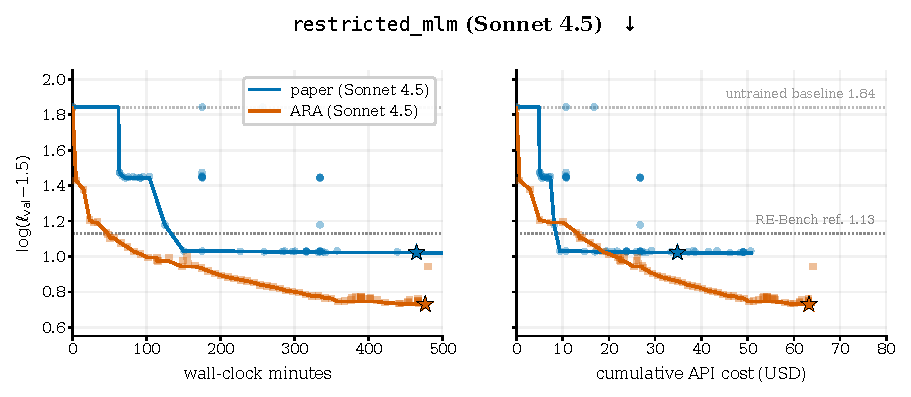
\includegraphics[keepaspectratio]{figures/extension/mlm_45_paper_vs_ara.pdf}}

}

\caption{\label{fig-extension-mlm-45}\passthrough{\lstinline!restricted\_mlm!}在Sonnet
4.5上：论文
vs.~Ara分数-时间（左）和分数-成本（右）。淡色标记为原始评分尝试，实线为迄今最佳包络线，星星标记最佳尝试位置。虚线标记未训练MLP基线（1.84）和RE-Bench参考值（1.13）。双方在\(t = 0\)时锚定在1.84基线；Ara-4.5的智能体前测试框架基线崩溃（损坏的起始检查点），智能体的第一个存活分数（\(t \approx 5\)分钟时1.43）反映轨迹推荐的\passthrough{\lstinline!ConvMLMWithBiBigrams!}架构已被换入（预计算的二元组表在未训练时得分\({\sim}1.43\)），我们将其锚定在1.84以匹配其他三个臂的实际基线测量值。Ara-4.5达到0.73
vs.~论文-4.5稳定在1.03------在较弱的基础上约30\%的相对领先。4.6轨迹在正文组合图中。}

\end{figure}%

\paragraph{跨模型版本的翻转。}\label{ux8de8ux6a21ux578bux7248ux672cux7684ux7ffbux8f6c}

\passthrough{\lstinline!restricted\_mlm!}是我们五个任务中唯一一个\textsc{Ara}-vs-论文的符号在模型之间翻转的任务：在Sonnet
4.5上，\textsc{Ara}智能体达到0.73 vs.~论文臂智能体的1.03；在Sonnet
4.6上，论文臂智能体达到0.69
vs.~\textsc{Ara}智能体的1.02。从4.5到4.6，论文臂智能体在同一任务上提高了约33\%，而\textsc{Ara}智能体降低了约40\%。

\paragraph{所有四个智能体中的相同架构家族。}\label{ux6240ux6709ux56dbux4e2aux667aux80fdux4f53ux4e2dux7684ux76f8ux540cux67b6ux6784ux5bb6ux65cf}

每次运行的最终\passthrough{\lstinline!solution/model.py!}包含一个\passthrough{\lstinline!BiBigramMLM!}类加一个\passthrough{\lstinline!ConvMLM*!}变体（论文-4.5：\passthrough{\lstinline!ConvMLMWithBiBigrams!}；\textsc{Ara}-4.5：\passthrough{\lstinline!ConvMLMComponent!}；论文-4.6：\passthrough{\lstinline!ConvMLMDilated!}；\textsc{Ara}-4.6：\passthrough{\lstinline!ConvMLMWithReLUAttn!}加五个其他变体）。所有四个都使用了二元组先验，来自启发式规则\passthrough{\lstinline!H04!}的\passthrough{\lstinline!as\_strided!}+\passthrough{\lstinline!einsum!}卷积，以及官方Tao配方。论文臂智能体也发现了正确的架构；分叉不在于架构上限。

\paragraph{差异在于是探索广度。}\label{ux5deeux5f02ux5728ux4e8eux662fux63a2ux7d22ux5e7fux5ea6}

四个\passthrough{\lstinline!model.py!}文件在大小和类数量上差异显著。论文-4.5：9.8
KB，3个类；\textsc{Ara}-4.5：8.9 KB，3个类；论文-4.6：6.3
KB，2个类；\textsc{Ara}-4.6：47
KB，6+个类（\passthrough{\lstinline!ConvMLMWithReLUAttn!},
\passthrough{\lstinline!ExtendedBiBigramMLM!},
\passthrough{\lstinline!ConvMLMWithLinearGlobal!},
\passthrough{\lstinline!ConvMLMWithGlobalContext!},
\passthrough{\lstinline!MLPMixerWithBiBigrams!},
\passthrough{\lstinline!ReLUAttentionMLM!}）。轨迹关键词计数反映了这一点：论文-4.6在整个运行中提及\passthrough{\lstinline!ReLU-attention!}一次，\passthrough{\lstinline!MLPMixer!}三次；\textsc{Ara}-4.6提及它们247次和73次。正文图
Figure~\ref{fig-extension-summary}最右列中的分数回归尖峰是可见的记录：每个朝向1.85或2.5的尖峰是一个新训练的替代架构被评分、发现有问题、被放弃，转而使用保存的最佳ConvMLM检查点。

\paragraph{\texorpdfstring{为什么\textsc{Ara}在Sonnet
4.5上获胜。}{为什么在Sonnet 4.5上获胜。}}\label{ux4e3aux4ec0ux4e48b58fc729-690b-4000-b19f-365a4093b2ff7b7b3c20617261203e7d7dux5728sonnet-4.5ux4e0aux83b7ux80dc}

两个4.5智能体最终都调优了相同的ConvMLM家族。\textsc{Ara}智能体的\passthrough{\lstinline!ThinkingBlock!}在\(t = 24\)分钟时明确承诺（\emph{``这应该足以击败参考分数1.13''}）并排队了40k
+
50k延续步骤。在\(t = 26\)分钟时，它将ReLU注意力搁置为\emph{``如果我想瞄准更高分的备选策略''}------对启发式规则的排序列表解读。拥有单一的主架构和一个经验上限（``没有MALT运行击败1.13''），\textsc{Ara}智能体在一个模型上花了约7小时持续微调并达到0.73。论文臂智能体没有等效的''没有先前智能体击败它''信号，没有对单一调优投入可比深度，稳定在1.03。胜利是在共享架构内由深度驱动的。

\paragraph{为什么论文臂智能体在Sonnet
4.6上获胜。}\label{ux4e3aux4ec0ux4e48ux8bbaux6587ux81c2ux667aux80fdux4f53ux5728sonnet-4.6ux4e0aux83b7ux80dc}

4.6智能体在架构上分道扬镳。论文臂智能体发明了\passthrough{\lstinline!ConvMLMDilated!}（一个在\passthrough{\lstinline!paper.md!}中未命名的扩张卷积变体），在前30分钟内对其承诺，并在整个8小时内运行单一微调，达到0.69。\textsc{Ara}智能体则实现了启发式规则层命名的额外架构------\passthrough{\lstinline!H11!}
ReLU注意力（\emph{``任何MALT运行用来击败参考值的唯一注意力替代方案''}）、\passthrough{\lstinline!H07!}
MLPMixer------并串行训练它们。在Sonnet
4.6的损失景观中，没有一个超越基本ConvMLM：\passthrough{\lstinline!H11!}和\passthrough{\lstinline!H07!}是从Claude-4
Sonnet基础的先前MALT运行派生的，对于一个优化方式不同的后继模型，菜单已经过时了。机制与4.5中相同------\textsc{Ara}智能体重视启发式规则命名的替代方案------但带宽差异翻转了其符号：4.5无法负担让次要条目成为主要条目的代价，因此它们充当带有备选的排序指针；4.6可以全部并行训练它们，菜单变成了一个碎片化的并行探索列表。

\subsection{可复现性}\label{sec-app-extension-repro}

所有实验构件和代码存放在项目仓库中：\passthrough{\lstinline!code/extension-harness/!}包含SLURM启动的测试框架、按任务系统提示和评分脚本以及分析图表生成器；\passthrough{\lstinline!code/rebench-pipeline/!}包含\textsc{Ara}编译流水线（规则、编排器过程和共享子智能体提示）；\passthrough{\lstinline!code/artifacts/rebench-<task>/!}包含每个任务的完整\textsc{Ara}和论文臂智能体的\passthrough{\lstinline!paper.md!}-加-\passthrough{\lstinline!src/!}捆绑包。每次运行的\passthrough{\lstinline!trace.jsonl!}是权威事件日志；本文中的每个分数、成本和图表都可以通过\passthrough{\lstinline!code/extension-harness/analysis/!}中的分析脚本从中重建。

\section{评审系统评估}\label{sec-app-review-system}

\subsection{ARA认证验证细节}\label{sec-app-seal-details}

\paragraph{认证实现。}\label{ux8ba4ux8bc1ux5b9eux73b0}

每个验证级别实现为一个自动化检查器：

\begin{itemize}
\tightlist
\item
  \textbf{级别1（结构完整性）}：一个Python脚本验证(a)
  必需目录的存在（\passthrough{\lstinline!/logic!},
  \passthrough{\lstinline!/src!}, \passthrough{\lstinline!/trace!},
  \passthrough{\lstinline!/evidence!}），(b)
  所有必需文件的存在，包括带有有效YAML前言部分的\passthrough{\lstinline!PAPER.md!}、\passthrough{\lstinline!problem.md!}、\passthrough{\lstinline!claims.md!}、\passthrough{\lstinline!experiments.md!}以及所有\passthrough{\lstinline!solution/!}文件，(c)
  每个结构化文件的模式一致性（例如每个论断必须具有\passthrough{\lstinline!Statement!},
  \passthrough{\lstinline!Status!},
  \passthrough{\lstinline!Falsification criteria!}和\passthrough{\lstinline!Proof!}；每个实验必须具有\passthrough{\lstinline!Verifies!},
  \passthrough{\lstinline!Setup!},
  \passthrough{\lstinline!Procedure!}和\passthrough{\lstinline!Expected outcome!}；每个启发式规则必须具有\passthrough{\lstinline!Rationale!},
  \passthrough{\lstinline!Sensitivity!}和\passthrough{\lstinline!Bounds!}），(d)
  最小计数（\(\geq 5\)个概念，\(\geq 3\)个实验，\(\geq 8\)个探索树节点，至少一个\passthrough{\lstinline![dead\_end]!}和一个\passthrough{\lstinline![decision]!}），以及(e)
  跨层引用解析：\passthrough{\lstinline!claims.md!}的\passthrough{\lstinline!Proof!}字段中引用的每个实验ID都解析为\passthrough{\lstinline!experiments.md!}中的一个条目；\passthrough{\lstinline!experiments.md!}的\passthrough{\lstinline!Verifies!}字段中引用的每个论断ID都解析为\passthrough{\lstinline!claims.md!}中的一个条目；\passthrough{\lstinline!heuristics.md!}中的每个\passthrough{\lstinline!code\_ref!}指向\passthrough{\lstinline!/src!}中的一个有效模块；\passthrough{\lstinline!architecture.md!}中声明的组件具有对应的代码桩；\passthrough{\lstinline!exploration\_tree.yaml!}中的论断引用解析为有效的论断ID。
\item
  \textbf{级别2（论证严谨性）}：在不执行代码或查阅外部来源的情况下，严谨性审计器在六个客观的、锚定在评分标准上的维度上评估构件的内容（证据相关性、可证伪性质量、范围校准、论证连贯性、探索完整性、方法论严谨性），每个维度按1到5分评分。输出是一份严谨性报告，定位到具体的\textsc{Ara}组件，包含按严重性排序的发现、逐字证据跨度以及从均值和每个维度下限导出的总评等级。
\item
  \textbf{级别3（执行可复现性）}：一个编码智能体读取\textsc{Ara}并尝试使用代码内核复现论断。LLM生成的测试用例验证论文论断的方向性属性。这与复现评估（\S\ref{sec-eval-reproduction}）中使用的是相同的协议。
\end{itemize}

\paragraph{失败分类。}\label{ux5931ux8d25ux5206ux7c7b}

对于每个认证级别的失败，我们记录失败的具体检查，并将其归类为以下类别之一：\emph{缺失文件}、\emph{缺失字段}、\emph{悬空引用}、\emph{类型不匹配}、\emph{依赖解析失败}、\emph{执行错误}或\emph{非确定性}。

\subsection{ARA认证有效性：评估细节}\label{sec-app-seal-eval}

本附录包含支撑\S\ref{sec-eval-seal}的方法论和按级别细分。

\subsubsection{级别1：编译器收敛数据}\label{sec-app-seal-eval-l1}

级别1验证结构正确性和完整性；我们通过在\textsc{Ara}生成和下游使用期间收集的两个复用信号来报告其有效性。

\paragraph{编译器迭代次数。}\label{ux7f16ux8bd1ux5668ux8fedux4ee3ux6b21ux6570}

23个PaperBench \textsc{Ara}和7个RE-Bench
\textsc{Ara}中的每一个都在编译器的生成--验证--修复循环（\S\ref{sec-ingestor}）的\(\leq 3\)次迭代内收敛到通过级别1。首次迭代通过率为0/30；所有构件需要至少一轮反馈，确认了级别1是一个有意义的过滤器而非橡皮图章。

\paragraph{失败类别分布。}\label{ux5931ux8d25ux7c7bux522bux5206ux5e03}

在所有编译器迭代中，级别1失败细分如下：悬空跨层引用（42\%）、论断、实验或启发式规则上的缺失模式字段（31\%）、\passthrough{\lstinline!exploration\_tree.yaml!}中节点计数不足（14\%）、YAML或前言部分解析错误（8\%）以及缺失必需文件（5\%）。该分布在论文之间是稳定的，并与附录
\ref{sec-app-seal-details}中的失败分类体系相匹配。

\paragraph{\texorpdfstring{以理解作为生成\textsc{Ara}上级别1的证明。}{以理解作为生成上级别1的证明。}}\label{ux4ee5ux7406ux89e3ux4f5cux4e3aux751fux6210b58fc729-690b-4000-b19f-365a4093b2ff7b7b3c20617261203e7d7dux4e0aux7ea7ux522b1ux7684ux8bc1ux660e}

理解评估（\S\ref{sec-eval-understanding}，表
\ref{tab-understanding}）是端到端的见证，证明级别1对生成的构件实施了它声称要实施的内容。每个进入该基准的\textsc{Ara}都已通过级别1；95.6\%的Cat.
A准确率则表明，经过级别1把关的\textsc{Ara}携带了智能体检索源中确实存在的信息所需的结构完整性。一个缺失必需字段或存在悬空跨层引用的构件将无法通过级别1并永远不会进入基准，因此4.4\%的残差受到源信息确实缺失的限制，而非构件的结构缺陷。

\subsubsection{级别2：变异基准测试}\label{sec-app-seal-eval-l2}

\paragraph{设置与评估标准。}\label{ux8bbeux7f6eux4e0eux8bc4ux4f30ux6807ux51c6}

级别2基准测试在\emph{被变异}的\textsc{Ara}上对严谨性审计器进行压力测试，因此报告的等级不携带真实值信号；我们严格按审计器是否将注入的缺陷作为发现浮出来评分。语料库为通过级别1的23个PaperBench
\textsc{Ara}；每个被注入每种类型一个（共115个变异）。所有注入记录在每个论文的\passthrough{\lstinline!injection\_manifest.json!}中，对审计器不可见。

\paragraph{注入模式。}\label{ux6ce8ux5165ux6a21ux5f0f}

五种类型针对不同的模式不变量：

\begin{itemize}
\tightlist
\item
  \textbf{虚构论断}：追加一个其\passthrough{\lstinline!Proof!}引用一个不存在实验ID的论断；信号
  = 悬空引用加上无依据的内容。
\item
  \textbf{缺失可证伪性}：从一个主要论断中删除\passthrough{\lstinline!Falsification criteria!}行；信号
  = 必需字段缺失。
\item
  \textbf{孤立实验}：追加一个其\passthrough{\lstinline!Verifies!}字段引用不存在论断ID（例如\passthrough{\lstinline!C99!}）的实验；信号
  = 证据不支持任何论断。
\item
  \textbf{过度论断}：将一个狭窄的\passthrough{\lstinline!Statement!}替换为全称范围模板，同时保持原始\passthrough{\lstinline!Falsification criteria!}和\passthrough{\lstinline!Proof!}不变；信号
  = 论断广度与证据覆盖之间的范围不匹配。
\item
  \textbf{被反驳分支泄露}：追加一个倡导\passthrough{\lstinline!trace/exploration\_tree.yaml!}标记为\passthrough{\lstinline!dead\_end!}的方法的论断；信号
  = 论断与探索记录之间的直接矛盾。
\end{itemize}

\paragraph{审计器与盲法化。}\label{ux5ba1ux8ba1ux5668ux4e0eux76f2ux6cd5ux5316}

严谨性审计器是一个智能体技能
\citep{agentskills2025}，按构件调用，仅授予构件目录；清单和源PDF被保留。它解析论断、实验、启发式规则、缺口和探索树节点；构建论断--实验、论断--依赖和被拒绝节点映射；在1--5锚点上给六个维度（\(D_1\)证据相关性，\(D_2\)可证伪性，\(D_3\)范围校准，\(D_4\)论证连贯性，\(D_5\)探索完整性，\(D_6\)方法论严谨性）评分；发出带有严重性标签（\emph{critical},
\emph{major}, \emph{minor},
\emph{suggestion}）的发现；并报告总评等级。完整技能规范（提示、锚点、阈值）随补充代码发布。

\paragraph{匹配与检出率。}\label{ux5339ux914dux4e0eux68c0ux51faux7387}

每个注入通过以下规则匹配至多一个发现：如果(a)其\passthrough{\lstinline!target\_entity!}等于注入的目标实体，或(b)其\passthrough{\lstinline!observation!}包含与注入唯一关联的文字标识符（例如孤立的\passthrough{\lstinline!C99!}，被反驳分支的注入死胡同节点ID），则发现命中。计数命中时忽略严重性和维度分配。按类型检出率（表
\ref{tab-seal-l2-heatmap}）为虚构论断、过度论断和被反驳分支泄露均为23/23；缺失可证伪性为21/23，两次漏检（\passthrough{\lstinline!bam!}
C02，\passthrough{\lstinline!bbox!}
C04）被静默重新归因到相邻维度；孤立实验为5/23------一个系统性盲点，我们将其归因于审计器以论断为中心的遍历方式，从不枚举没有入向\passthrough{\lstinline!Verifies!}边的实验。

\begin{table*}[t]
\centering
\small
\begin{tabular}{l | c c c c c}
\toprule
\textbf{论文} & \textbf{虚构} & \textbf{缺失可证伪} & \textbf{孤立} & \textbf{过度论断} & \textbf{被反驳} \\
\midrule
adaptive-pruning                           & \cmark & \cmark & \cmark & \cmark & \cmark \\
all-in-one                                 & \cmark & \cmark & \cmark & \cmark & \cmark \\
bam                                        & \cmark & \xmark & \cmark & \cmark & \cmark \\
bbox                                       & \cmark & \xmark & \xmark & \cmark & \cmark \\
bridging-data-gaps                         & \cmark & \cmark & \xmark & \cmark & \cmark \\
fre                                        & \cmark & \cmark & \xmark & \cmark & \cmark \\
ftrl                                       & \cmark & \cmark & \xmark & \cmark & \cmark \\
lbcs                                       & \cmark & \cmark & \xmark & \cmark & \cmark \\
lca-on-the-line                            & \cmark & \cmark & \xmark & \cmark & \cmark \\
mechanistic-understanding                  & \cmark & \cmark & \xmark & \cmark & \cmark \\
pinn                                       & \cmark & \cmark & \xmark & \cmark & \cmark \\
rice                                       & \cmark & \cmark & \xmark & \cmark & \cmark \\
robust-clip                                & \cmark & \cmark & \xmark & \cmark & \cmark \\
sample-specific-masks                      & \cmark & \cmark & \xmark & \cmark & \cmark \\
sapg                                       & \cmark & \cmark & \cmark & \cmark & \cmark \\
self-composing-policies                    & \cmark & \cmark & \xmark & \cmark & \cmark \\
self-expansion                             & \cmark & \cmark & \xmark & \cmark & \cmark \\
semantic-self-consistency                  & \cmark & \cmark & \xmark & \cmark & \cmark \\
sequential-neural-score-estimation         & \cmark & \cmark & \xmark & \cmark & \cmark \\
stay-on-topic-cfg                          & \cmark & \cmark & \xmark & \cmark & \cmark \\
stochastic-interpolants                    & \cmark & \cmark & \xmark & \cmark & \cmark \\
test-time-model-adaptation                 & \cmark & \cmark & \xmark & \cmark & \cmark \\
what-will-my-model-forget                  & \cmark & \cmark & \xmark & \cmark & \cmark \\
\midrule
\textbf{总检出 (/23)} & \textbf{23} & \textbf{21} & \textbf{5} & \textbf{23} & \textbf{23} \\
\bottomrule
\end{tabular}
\caption{级别2变异基准测试的按论文$\times$按注入检出情况。\cmark{} = 已检出；\xmark{} = 漏检。孤立实验列揭示了\S\ref{sec-eval-seal}中讨论的系统性盲点。}
\label{tab-seal-l2-heatmap}
\end{table*}

\paragraph{诊断：分数-发现脱钩。}\label{ux8bcaux65adux5206ux6570-ux53d1ux73b0ux8131ux94a9}

尽管等级不是评估标准，审计器的评分行为对未来的迭代是有参考价值的。在被反驳分支泄露被标记为\emph{critical}级\(D_5\)发现的22个\textsc{Ara}上，审计器仍然分配\(D_5 \in \{3,4\}\)，尽管锚点规定1（``树与论断矛盾''）或2（``样板文档''）。行文中的严重性未传播到数值分数。下一版本的教训是机制性的：维度分数应从发现列表中导出，而不是由智能体独立报告。

\subsubsection{级别3：执行可复现性}\label{sec-app-seal-eval-l3}

级别3有效性等同于复现评估（\S\ref{sec-eval-reproduction}, 附录
\ref{sec-app-reproduction-eval}）：一个编码智能体读取\textsc{Ara}并尝试使用代码内核复现论断，通过LLM生成的测试用例进行方向性验证。我们将表
\ref{tab-repro-per-difficulty}中报告的按论文难度加权复现分数作为级别3信号，并请读者参考附录
\ref{sec-app-reproduction-eval}了解任务设计、评分和按论文分析。

\paragraph{\{=html\} 直写表格的 PDF
端转换测试}\label{html-ux76f4ux5199ux8868ux683cux7684-pdf-ux7aefux8f6cux6362ux6d4bux8bd5}

以下表格以 \{=html\} 直写（非 LaTeX、非管道表），用于验证 paper-tables
扩展的 HTML raw → LaTeX 兜底转换（PDF 端经 pandoc.read 解析为 Table AST
后按 booktabs 三线表输出）：

\begin{table}[htbp]
\centering
\begin{tabular}{lll}
\toprule
方法 & Q\&A 准确率 & 复现成功率 \\
\midrule
ARA & 93.7\% & 64.4\% \\
基线 & 72.4\% & 57.4\% \\
\bottomrule
\end{tabular}
\caption{HTML 直写表格的 PDF 端转换测试}
\label{tab-html-raw-test}
\end{table}




\end{document}
